\documentclass{article}
\usepackage[utf8]{inputenc}
\usepackage{geometry}
\usepackage{graphicx}
\usepackage[table,xcdraw]{xcolor}
\usepackage{multicol}
\usepackage{multirow} % weird table stuff
\usepackage{array}
\usepackage{wrapfig} % package for wrapping figures
\usepackage{float} % adds 'H' identifier for figures etc
\usepackage{setspace} % helps with multiple column table of contents idk why
\usepackage{soul} % to highlight stuff with \hl{}
\usepackage[hyphens]{url} % Used to make urls breakable and breaks them at a hyphern
\usepackage[hidelinks]{hyperref} % Allows for use of urls and related characters in references, doesn't put a box around links
\hypersetup{breaklinks=true} % Allows for links to be broken
\usepackage{eso-pic} % for front page top right logo

\usepackage[format=plain,
            labelfont={bf},
            textfont=it,
            justification=centering]{caption} % Package for managing captions. Makes the label bold and all the caption italic and centered

\parskip=8pt % Sets the paragraph spacing between paras
\parindent=0pt % disables indentation

\geometry{
    a3paper,
    twocolumn,
    landscape,
    hmargin={2cm, 2cm},
    vmargin={2cm,2cm},
    footskip=0.75cm,
    headsep=0.25cm
}

\setlength{\columnseprule}{0pt}
\setlength{\columnsep}{1.3cm} % separation in between columns

\newcommand{\CellColor}{a7c3d4} % color of tables (Hex)

%---------------------------------------------------------------------------------
%---------------------------------------------------------------------------------

\title{GDP report} % disregard
\date{12\textsuperscript{th} of May 2022} % disregard

%---------------------------------------------------------------------------------
%---------------------------------------------------------------------------------

\begin{document}

%\maketitle

\begin{center}

\newcommand{\HRule}{\rule{\linewidth}{0.5mm}} % Defines a new command for the horizontal lines, change thickness here

\center % Centre everything on the page

\textsc{\LARGE University of Southampton}\\[7mm] % Name of your university/college

\includegraphics[scale=.17]{images/crest.jpg}\\[0.5cm] % Include a department/university logo - this will require the graphicx package
\textsc{\Large Aeronautics \& Astronautics}\\[0.15cm] % Major heading such as course name
\textsc{\large Faculty of Engineering and Physical Sciences}\\[0.2cm] % Minor heading such as course title

\HRule \\[4mm]
{ \huge \bfseries FEEG6013}\\[0.4cm]
{ \huge \bfseries GDP Group 17}\\[0.4cm]
{ \huge \bfseries Downwind-Faster-Than-The-Wind}\\[0.4cm]
\HRule \\[6mm]

Group Members:\\
\textbf{\emph{Hadrien DEVELAY -} 29323738}\\
\textbf{\emph{Jean FESQUET -} 29370272}\\
\textbf{\emph{James FOGGIN -} 29652987}\\
\textbf{\emph{Alexander HOAD -} XXXXXXXX}\\
\textbf{\emph{Iwan TOMOS -} 30141508}\\
\textbf{\emph{Simeon YOUNG -} 29977916}\\[12mm]

Primary Supervisor: \textbf{\emph{Davide LASAGNA}}\\
Co-Supervisor: \textbf{\emph{Ivo PETERS}}\\[12 mm]


%\vfill % Fill the rest of the page with whitespace


Submitted on May 12\textsuperscript{th}, 2022\\[12mm] % Date, change the \today to a set date if you want to be precise

\end{center}

%\tableofcontents
\begin{multicols}{2}
\setstretch{1}{
    \parskip=0em
    \setlength{\columnseprule}{0.4pt}   % Puts lines between the columns to make it easy to read (can be removed)
    \tableofcontents
    }
\end{multicols}
\newpage

\section*{Acknowledgements}

We would like to extend our gratitude to our supervisors, Dr Davide Lasagna and Dr Ivo Peters, for giving us the opportunity to work on this exciting project, and for providing regular feedback and encouragement in weekly meetings.

Additionally, we would like to thank Dr David Marshall, Renan Soares, Sam Harper, and Andy Ferady for allowing us to use the R.J. Mitchell wind tunnel on multiple occasions, and the exceptional efforts of Dr David Marshall to meet with us and provide professional expertise to aid the project.

We would also like to thank the University of Southampton EDMC for their assistance in the manufacture of components and the assembly of the vehicle.


%\newpage

\vspace{4cm}

\begin{center}
\rule{0.6\linewidth}{0.4pt}
\end{center}

\vspace{4cm}


\section{Introduction}
This group design project has focused on building a downwind faster than the wind (DWFTTW) vehicle. Although the working principles of this type of vehicle are not obvious, this concept has been proven to work on numerous occasions, both theoretically and experimentally. This has been done by multiple reliable sources. One of which is Prof Mark Drela's theoretical analysis of the working principle of the vehicle. Furthermore, a racing competition for this kind of vehicle has been held annually since 2018, in which multiple universities have taken part. The vehicle is composed of a set of wheels connected mechanically to a propeller. As the wind pushes the vehicle and speed builds up, the propeller receives torque from the wheels and propels the vehicle further. This allows the vehicle to reach speeds that can be faster than that of the wind. The theoretical aspect of this will be detailed in the Theory section.

\subsection{Project Inspiration}

Major inspiration for this project came from a YouTube video uploaded by Veritasium (a well-known science and engineering channel) focussed on a DWFTTW vehicle called BlackBird. Its inventors, Rick Cavallaro and John Borton, demonstrated their vehicle on the Ivanpah dry lake bed, south of Las Vegas, and achieved almost three times wind speed. Despite numerous demonstrations of DWFTTW vehicles beating wind-speed, scepticism among the scientific community exists to this day, with the commonly held belief that a vehicle with faster-than-wind capabilities would be a perpetual motion device, violating the first law of thermodynamics. One of the ways to tackle this scepticism is to make such vehicles more widely known by building and demonstrating additional working prototypes.

\subsection{Existing Vehicles}

\textcolor{red}{
    Find any DWFTTW vehicle examples
    Look in detail at the designs and include them in the vehicles section
    Find appropriate pictures of each vehicle
    Read the papers on the DWFTTW vehicles and write literature review on the papers (jean pending)
}

\subsection{Aeolus Competition}

The Aeolus competition is an annual drag race competition for downwind faster than the wind vehicles. The teams collect together and compete for the fastest vehicle. The competition ran in 2018 and 2019 with many teams entering.

We have taken inspiration from this competition in wanting to build a downwind faster than the wind vehicle, with our vehicle being the first iteration for the university competing in this competition.

Although Pam is unmanned, and a smaller scale compared to the maximum limits in the rulebook, the design was thought to be scalable. 

\subsection{Previous Attempts at Downwind-Faster-Than-The-Wind Vehicles}

See Table \ref{tab:prevAttempts}.

%\onecolumn
\newcommand\x{3.5cm} %set cell width
\begin{table}[p]
    \centering
    \begin{tabular}{|m{5cm}|m{\x}|m{\x}|m{\x}|m{\x}|m{\x}|m{\x}|m{\x}|m{\x}|}
      \hline
      \textbf{Design} &
      \textbf{Cost} &
      \textbf{Aesthetics} &
      \textbf{Modularity} &
      \textbf{Manufacturability} &
      \textbf{Safety} &
      \textbf{Performance} &
      \textbf{Complexity} &
      \textbf{Durability} 
      \\ \hline
      
      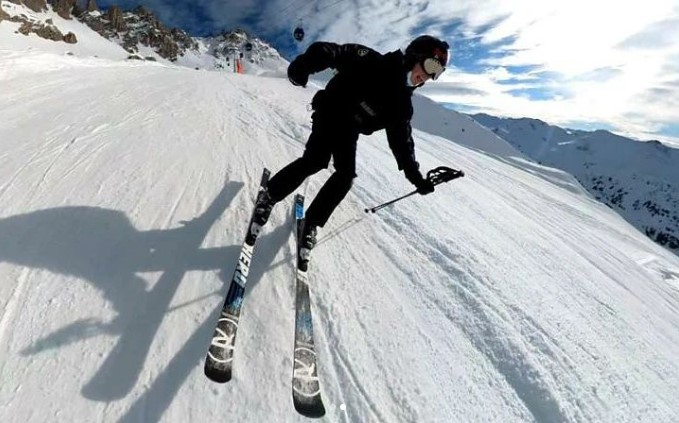
\includegraphics[width=\linewidth]{images/placeholder.jpg}
      &
      The cost of this vehicle could be larger than the other vehicles due to the aerodynamic body of the vehicle and the fact that there are two propellers. The dual prop design would also increase the amount of components in the drivetrain, increasing the cost.
      & 
      The finish is relatively clean for this vehicle, which improves the overall aesthetics. From analysis the streamlined body of the vehicle would add significant designing, to the project. 
      &  
      The drivetrain of this vehicle looks relatively modular, with the main structure being connected with bolts. The two-propeller system reduces the modularity of the vehicle.
      & 
      The two propellers would be able to be manufactured in tandem, but a significant amount of manufacturing would have to be completed to finish the vehicle.  
      &  
      The vehicle looks relatively stable, although the propeller looks relatively large in comparison to the vehicle which could cause oscillatory issues.
      &  
      The two-propeller system would generate a significant amount of thrust. 
      &  
      The vehicle is very complex with two propellers adding significant design for the drivetrain and the aerodynamics of the vehicle. 
      &  
      The vehicle has a lot of aerodynamic components that could be broken easily and would need to be replaced. Initially designing the vehicle for durability will therefore help improve the project, especially with us focussing on durability.
      \\ \hline
      
      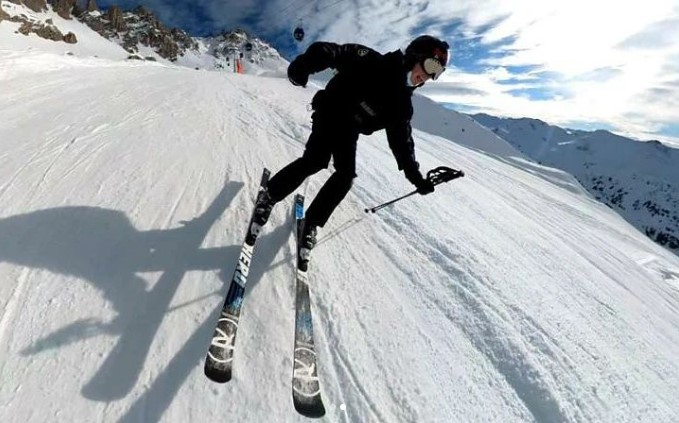
\includegraphics[width=\linewidth]{images/placeholder.jpg}
      &
      This vehicle looks very expensive due to the slick and streamlined nature of the body. The wheels are solid on this vehicle which would increase the expense of the vehicle significantly.
      &  
      The vehicle looks very aesthetically pleasing with the enclosed cockpit for the driver. The wheel covers add more to the design and make the vehicle look well engineered. 
      &  
      This vehicle doesn't look very complex. This is probably due to the fact that this vehicle is near the end of the design process and all components have been tested multiple times. 
      &  
      This vehicle will be difficult to manufacture. The aerodynamic body will have been made from a composite and the translucent window at the front will have been difficult to create. 
      &  
      This vehicle looks safe due to its enclosed cockpit design. The vehicle looks stable and there are obvious safety concerns that have been addressed on the vehicle. 
      &  
      This vehicle looks like it would performance well aerodynamically. The solid wheels will reduce the unpredictable nature of the wheels but will require additional suspension for the vehicle to run smoothly on the road. 
      &  
      The drivetrain system for this device looks like a shaft drive due to the thin pole supporting the vehicle. 
      & 
      As with the other vehicles, the outer casing will cause significant issues with durability, especially as composites can break with impacts. The wheels on this vehicle are an interesting prospect. 
      \\ \hline
      
      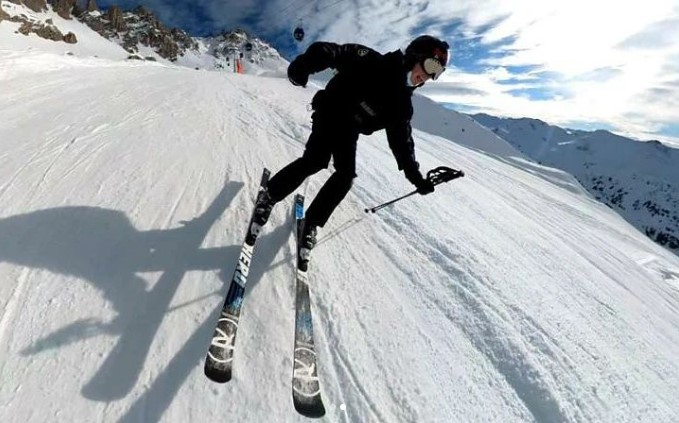
\includegraphics[width=\linewidth]{images/placeholder.jpg}
      &  
      This is the main vehicle that started the downwind faster than the wind theory. The propeller on this vehicle is large, therefore will cost a lot, adding to the already complex body.
      &  
      This vehicle looks relatively bulky but the significant aerodynamic components help improve the aerodynamics significantly. 
      &  
      As the vehicle has significant aerodynamic components that have been improved over a large amount of time, meaning most of the parts aren't replaceable. This vehicle isn't modular, and therefore takes a lot of work to maintain.
      &  
      Due to the complex components on this vehicle, this vehicle will be difficult to manufacture. On the whole the vehicle is complex to manufacture and is not a good vehicle to base our vehicle on.
      &  
      The YouTube video on this vehicle show significant oscillation when the propeller is moving quickly. The vehicle is not completely safe and has systems involved to stop the vehicle. Our vehicle is unmanned; therefore, these concerns will not be as significant. 
      &  
      This vehicle has shown incredible performance with good ability going upwind and downwind. The chain system on the vehicle provides significant tension for the propeller and spins and provides thrust at most speeds. 
      &  
      The vehicle is very complex in both aerodynamics and functionality. The vehicle can fold in half due to its size and need to be transported. The drivetrain of the vehicle although hidden is very complex and has been worked on for a long time.
      &  
      The vehicle is very large and components are state of the art for the vehicles, suggesting that they are not easily replaces. The vehicle frame is mechanical and therefore is prove to failure, and the structure is built from wood which with an impact could break 
      \\ \hline
    \end{tabular}
    \caption{Previous attempts at downwind-faster-than-the-wind vehicles}
    \label{tab:prevAttempts}
\end{table}
\twocolumn
% currently located in 2.designSpecs.tex for spatial reasons

\section{Project Aims and Objectives}
\subsection{Project Aims}

\begin{itemize}
    \item Design, build and test a wind-powered vehicle capable of travelling downwind faster than the wind with the vehicle able to be tested in the University's wind tunnel facilities.
    \item Gain a better understanding of downwind faster than the wind vehicles and the parameters that influence their performance.
\end{itemize}

\subsection{Project Objectives}

\begin{itemize}
\item Research all aspects of the vehicle, considering the performance losses at each state to make suitable and justifiable design decisions.
\item Understand the forces acting on the vehicle and explain how the vehicle functions.
\item Design an efficient drivetrain that can transfer rotational energy from the wheels to the propeller.
\item Design a system to vary the pitch of the propeller blades.
\item Design a modular vehicle that allows for modifications and developments during the project, after testing but also in further projects.
\item Complete the vehicle within budget.
\item Test the vehicle in the wind tunnel to acquire data on its performance.
\item Analyse wind tunnel data to validate theory/inform on areas of discrepancy and improvement
\end{itemize}






\section{Design Brief and Specifications}
\subsection{Design Criteria}

See Table \ref{tab:desigCrit}

%% Please add the following required packages to your document preamble:
% \usepackage[table,xcdraw]{xcolor}
% If you use beamer only pass "xcolor=table" option, i.e. \documentclass[xcolor=table]{beamer}
\begin{table}[H]
\centering
\caption{Design criteria}
\label{tab:desigCrit}
\begin{tabular}{|
>{\columncolor[HTML]{\CellColor}}l |p{14cm}|}
\hline
Design criteria   & \cellcolor[HTML]{\CellColor}Reasoning                                                                                                                                                                                                                                                                                                                                                                                      \\ \hline
Durability        & The durability of the vehicle was important to the project as developing a vehicle that is resilient and doesn’t deteriorate over time would allow for more testing. Having a vehicle that lasts the entire wind tunnel testing schedule is critical for this project as this would allow us to analyse data and complete the project aim of understanding the physical attributes of a downwind vehicle. \\ \hline
Cost              & The overall budget of the project was £850, which gave the project a constraint on the amount that we can feasibly spend on the vehicle. For this criterion it was critical to complete a vehicle under the amount of money available.\\ \hline
Manufacturability & As physically testing the vehicle in the R.J. Mitchell wind tunnel was set out as a goal from the outset of the project, ensuring the feasibility of manufacture of the vehicle was key.                                                                                                                                                                \\ \hline
Design            & The design of the vehicle needs to be well thought out as part of a suitable design process and any design decision justified accordingly with supporting data.                                                                                                                                                                                                                                                                                                                        \\ \hline
Performance       & The vehicle performance was a key factor for the project as seeing what thrust levels and efficiencies were part of the vehicle will help us understand the limitations of the concept. We aim to see the vehicle generating some level of thrust and acceleration within a range of speeds during the testing phase.                                                                                     \\ \hline
Aesthetics        & The aesthetics of the vehicle do not affect the performance when testing, but generally a good-looking vehicle was preferred as this was seen as a sign of a good project.                                                                                                                                                                                                                                                                                     \\ \hline
Complexity        & Minimizing the complexity of the vehicle will help the project as this will ensure that the vehicle will be able to be manufactured in time for the wind tunnel testing. Following this, basic concepts are easier to analyse with simpler designs which was though to be a priority for testing during the project.                                                                                                                                                                                                   \\ \hline
Safety            & Ensuring that the students and facility members are safe was a key focus for the project. Ensuring that all aspects of the project are safe before testing is critical and risk assessment will be completed before testing.                                                                                                                                                                                                                     \\ \hline
Modularity        & Having a vehicle that can be adapted easily will help the design process and allow for updates to be made to the vehicle. Having a vehicle that can be adapted with during the project will help the progress of the vehicle and enhance the project outcomes.                                                                                                                                                                                                    \\ \hline
\end{tabular}
\end{table}
% Please add the following required packages to your document preamble:
% \usepackage[table,xcdraw]{xcolor}
% If you use beamer only pass "xcolor=table" option, i.e. \documentclass[xcolor=table]{beamer}
\newcommand{\disregardCell}{\cellcolor[HTML]{C0C0C0}}
\begin{table}[!htbp]
\centering
\caption{Design criteria}
\label{tab:desigCrit}
\begin{tabular}{|p{3cm} |p{13.8cm}|}
\hline
\cellcolor[HTML]{\CellColor}\textbf{Design criteria}   & \cellcolor[HTML]{\CellColor}\textbf{Reasoning}
\\ \hline
\textbf{Performance}: reach ground speed higher than wind speed    
& 
In this project, the term `performance' relates directly to how fast the vehicle can travel downwind, compared to the speed of the wind. The objective of this project is to build a vehicle capable of travelling at a ground speed equal or superior to 100\% the speed of the wind, downwind.
\\ \hline
\textbf{Cost}: budget limit is \pounds850              
& 
The overall budget of the project is \pounds850, which gave the project a constraint on the amount that can feasibly be spent on the vehicle. For this criterion it was critical to complete a vehicle under the amount of money available.
\\ \hline
\textbf{Scale}: 80 cm propeller diameter       
& 
A main objective of the project is to test the vehicle in the R.J. Mitchell, hence a reasonably scaled model should be considered. Hence the propeller diameter was constrained to a maximum of 80 cm. The vehicle was thus built around this dimension. 
\\ \hline
\textbf{Durability}        
& 
The durability of the vehicle was important to the project as developing a vehicle that is resilient and does not deteriorate over time would allow for consistent testing. Having a prototype able to sustain wind tunnel testing was critical for this project. This way, data could be analysed and the aim of understanding the physical attributes of such vehicle, achieved. 
\\ \hline
\textbf{Safety}            
& 
Ensuring that the students and facility members were safe was a key focus for the project. This was achieved through thorough reviewing of the structural integrity of the prototype and rigorous compliance with relevant health and safety guidelines.
\\ \hline
\textbf{Modularity}        
& 
Having a vehicle that could be adapted easily helped the design process and allowed for updates to be made to the vehicle. Adapting the prototype during the project facilitated progress and enhanced project outcomes.
\\ \hline
\end{tabular}
\end{table}

\subsection{Project Life Cycle and Relevance}

This project is the first iteration of the University of Southampton building a downwind faster than the wind vehicle, with no record of previous work taking place. The current project aimed to design and manufacture a vehicle that could be tested at the University's facilities. This project aimed to understand the workings of a downwind faster than the wind vehicle and produce a starting point for projects within the University focused on downwind faster than the wind motion.



\subsection{Project Context}

With the global transportation market moving towards more sustainable forms of travel, the demand for renewable energies is becoming ever-growing. The potentially self-sustaining nature of these vehicles offers opportunities in the transportation sector to provide a green alternative to fossil fuels. In their current form, these vehicles are still early in development and do not provide a convenient solution, but a significant input into design could see many aspects implemented into sustainable travel in the future. The mechanical systems involved with these vehicles are not limited to land vehicles, with revisions in design being applicable to watercraft.

\subsection{Project Stakeholders}

See Table \ref{tab:stakeholders}.







\section{Project Management and Methodology}
\subsection{Project structure}

Analysing the requirements of the vehicle helped visualise the four main components of the project: structure, propeller, drivetrain, and pitch control mechanism. A high level of communication was required and, therefore, maintained between the teams working on the different components of the prototype. From the outset of the project, it was planned that the vehicle would be tested experimentally, therefore, planning of the experimental setups began during the later stage of the design process.

Once the designs were complete, manufacturing the drivetrain became an integral part of the project to ensure that the vehicle would be ready for the wind tunnel test. More focus was put on manufacturing to increase progress made on the vehicle before testing. To ensure all aspects of testing were accounted for, an emphasis was put on planning. After deciding on using the wind tunnel facility, a comprehensive plan was laid out for the tests, data collection and data processing.

Once the first wind tunnel test was complete, it was clear that there were still aspects of the vehicle that needed changing prior to the second test. Furthermore, with the overall timescale for the project reducing, it was important to start the analysis of the project outputs. Between wind tunnel tests the focus shifted to improving the vehicle and testing the new features that were implemented.

\subsection{Design Methodology}

\begin{figure}[!htbp]
    \centering
    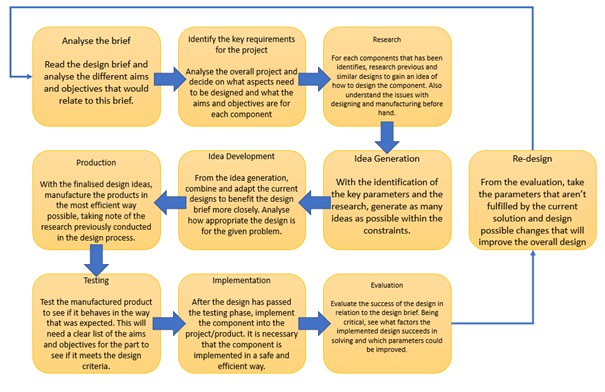
\includegraphics[width=0.7\linewidth]{images/part2/designMethodology.png}
    \caption{Design methodology flow chart}
    \label{fig:desmeth}
\end{figure}

The design methodology for the project focused on employing an iterative method to maximize the outcomes for the vehicle. Following Figure \ref{fig:desmeth} the project was run through this process, ensuring that each stage of design was evaluated properly and that additions to the design were thought out adequately. The project was conducted on a limited budget which enhanced the need to design the vehicle thoughtfully and limit the number of prototypes. Enhancing the vehicle by adding singular improvements sequentially helped reduce the budgetary requirements of the project and reduce overall costs. Working through the structure laid out in Figure \ref{fig:desmeth} was facilitated by the modular nature of the vehicle, as slight improvements could be well thought out before being implementation. Strong communication within the team was important as the performance of the prototype was highly dependent on the synergy between each of its components.

\subsection{Project Timings}

% \begin{figure}[h]
%     \centering
%     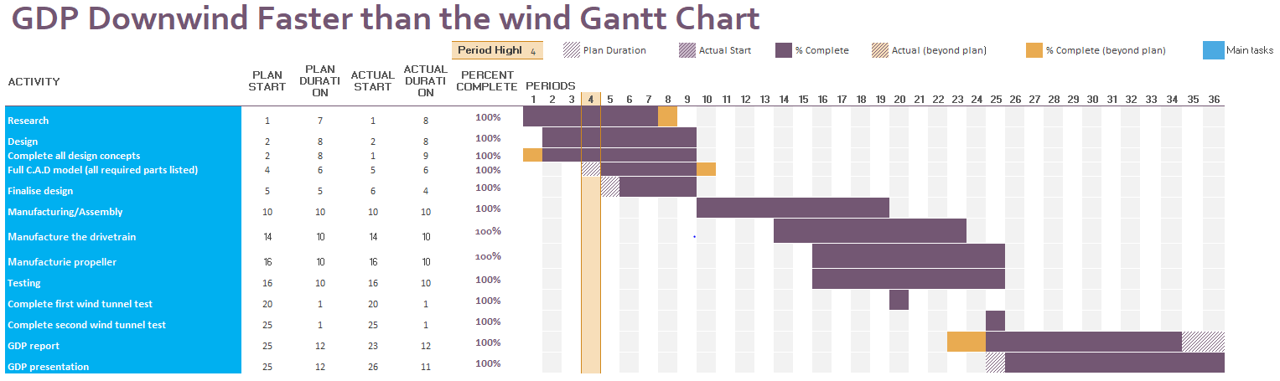
\includegraphics[width=\linewidth] {images/part2/gantt.png}
%     \caption{Gantt chart for project planning}
%     \label{fig:ghantt}
% \end{figure}

This project was run in three main phases: design, manufacture and testing. During the design phase, research was conducted on the various components of the vehicle. This was done in an effort to better understand the workings of the concept as well as maximize the performance of the final output. After research was completed, the information gathered was used in the flow chart of Figure \ref{fig:desmeth} to design the basic vehicle and then iterate through to finalize the project. After completion, the designs were sent to EDMC for manufacturing and finalized post receiving components. The final phase of the project was to test the vehicle, looking at evaluating the performance and understanding the limitations of the design.

\onecolumn
\begin{table}[p]
\caption{Project stakeholders}
\label{tab:stakeholders}
\centering
\begin{tabular}{|
>{\columncolor[HTML]{\CellColor}}l |p{13cm}|p{13cm}|}
\hline
\cellcolor[HTML]{\CellColor} &
  \cellcolor[HTML]{\CellColor}\textbf{Specific   Information Needs} &
  \cellcolor[HTML]{\CellColor}\textbf{Stakeholder   needs and Interests} \\ \cline{2-3} 
\multirow{-2}{*}{\cellcolor[HTML]{\CellColor}\textbf{Project stakeholder name}} &
  \cellcolor[HTML]{\CellColor}\textbf{Types \& Frequency of   Communication} &
  \cellcolor[HTML]{\CellColor}\textbf{Specific areas of interest and participation} \\ \hline
\textbf{Supervisors} &
  Organising weekly meetings with the project supervisors and giving them presentations on the progress of the project in each period was key to the progress of the project. Asking questions and receiving feedback on progress allows for the supervisors to provide detailed analysis and suggestions for improvements for the project. The supervisor's interest in the project is derived from their involvement in the Engineering discipline as researchers at the University &
  This project is derived from the downwind faster than the wind vehicle blackbird created by Rick Cavallaro. The supervisors affect the design of the vehicle directly by inputting their expertise into the project, helping the team understand flaws in their methods \\ \hline
\textbf{Team members} &
  The team members need to stay in contact constantly throughout the project to ensure the project runs   smoothly. Deciding the team roles early on was key for the project as it allowed each team member to know whom to contact with different issues. &
  The team members oversee running the project and ensure the final prototype is up to the standard. The aim is to create a downwind faster than the wind vehicle that runs at the highest speed as is possible. The team were in charge of building the vehicle and will therefore have direct input throughout the project on the design and were the largest contributors affecting the final outcome \\ \hline
\textbf{EDMC} &
  The EDMC team oversaw the manufacturing of all complex components for the vehicle. It was required for the team to stay in contact with the EDMC constantly while parts were being manufactured to ensure that appropriate timescales were upheld for job completion and when they needed any additional information for jobs. &
  The EDMC team were interested in all GDP projects for the university especially in completing project outputs and testing. They have a duty to help each team therefore want to complete all tasks in time as efficiently as possible. Ensuring that the communication was clear was key for this stakeholder as many jobs are submitted to the EDMC throughout the year. This stakeholder has an influence on the design of the project, as over-complicated designs require revision to successfully manufacture components\\ \hline
\textbf{Wind Tunnel team} &
  The main contact for the wind tunnel was David Marshall, the wind tunnel manager. Staying in weekly   contact with him throughout the project was helpful in maintaining a relationship with the facility team and ensuring that all members know the project well, allowing them to help the functionality of test days and achieve better results. &
  The wind tunnel team are interested in the project as the vehicle was run in the RJ Mitchell test   facility. They wanted to ensure that the project didn't damage their wind tunnel, therefore affecting the design by ensuring that the vehicle is safe. They were also interested in the practical outcome of the vehicle due to their involvement in aerodynamic testing. \\ \hline
\textbf{Suppliers} &
  The communication with any possible supplier was held until the components were needed for the vehicle. The frequency of the communications varied depending on the issues that arose from the designing and testing of the vehicle &
  The main interest of the suppliers of components was selling the product to the group. After the components were bought, their interest was directed to the component remaining functional for the buyer. \\ \hline
\end{tabular}
\end{table}
\twocolumn


\section{DWFTTW Working Principle}
The aim of this section was not to prove that this vehicle was not a perpetual motion machine but to briefly explain its working principles. Literature detailing sufficient proofs have already been given by reliable sources for the scepticism about this concept to be considered unreasonable.

\begin{figure}[!htbp]
    \centering
    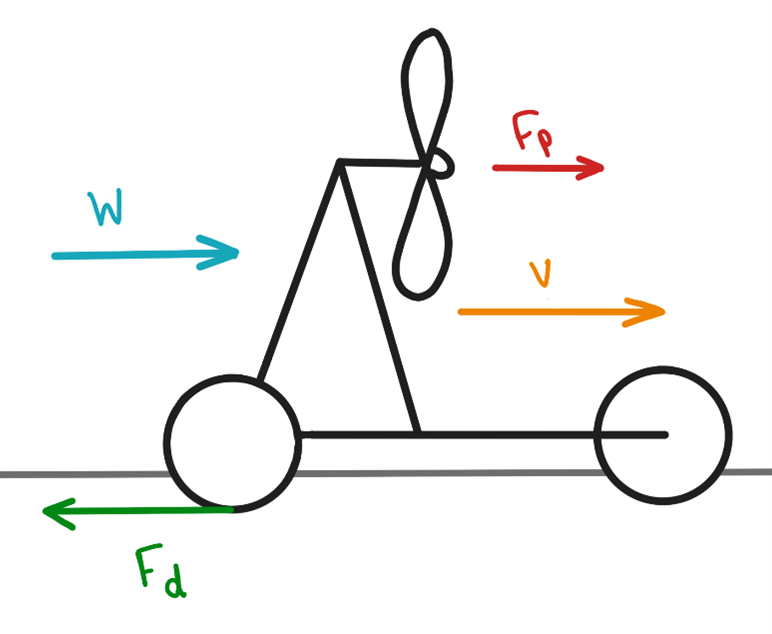
\includegraphics{images/part4/simplediag.png}
    \caption{Downwind Faster Than The Wind (DWFTTW) vehicle concept diagram}
    \label{fig:diagram}
\end{figure}

A Downwind Faster Than the Wind vehicle’s principle of operation is composed of four main events. First, the wind pushes the stationary vehicle. Second, the rotating wheels of the vehicle lead the chain connected to a propeller shaft. Third, the propeller spins and produces thrust. Approaching the wind speed, the propeller generates thrust even when the relative wind is zero, accelerating the vehicle until an equilibrium point between thrust and drag is reached. This point may be slower, equal to, or faster than the wind speed based on the efficiency of the vehicle components. It is important to emphasize that contrary to common belief, the rotor acts as a propeller producing thrust driven by the wheels, and is not a turbine extracting wind power to drive the wheels. This is the only difference between an upwind and a downwind vehicle as discussed earlier.

A set of equations were defined by Mark Drela in his “Dead Downwind faster than the wind analysis” \cite{drela20dead}. Where $F_p$ is the thrust provided by the propeller and $F_d$ is the force extracted from the ground as a result of the vehicle being pushed by the wind. The power outputted by the wheels and used by the propeller can be defined as follows. This introduces the overall propeller efficiency $\eta_p$.

\begin{equation}
P_{d}=F_{d} V
\label{eq:a}
\end{equation}

\begin{equation}
P_{p}=\frac{F_{p}(V-W)}{\eta_{p}}
\label{eq:b}
\end{equation}

Balancing both powers introduces a new efficiency coefficient $\eta_g$ which corresponds to the overall transmission efficiency between the wheels and the propeller.

\begin{equation}
    P_p = P_d \eta_g
    \label{eq:c}
\end{equation}

Substituting the forces defined in Equations \ref{eq:a} and \ref{eq:b} yields Equation \ref{eq:d} which is the simplified relationship between the propeller thrust and the wheel force:

\begin{equation}
F_{p}=F_{d} \frac{V}{V-W} \eta_{g} \eta_p
\label{eq:d}
\end{equation}

The net force on the vehicle is defined by Drela as the thrust generated by the propeller minus the force from the wheels. This leads to Equation \ref{eq:e} as follows:

\begin{equation}
    F_{net} = F_p - F_d
    \label{eq:fnet}
\end{equation}

\begin{equation}
F_{n e t}=F_{d}\left(\frac{V}{V-W} \eta_{g} \eta_{p}-1\right)
\label{eq:e}
\end{equation}

So long as the following coefficient is greater than one, the vehicle can be faster than the wind:

\begin{equation}
\frac{V}{V-W} \eta_{g} \eta_{p}>1
\label{eq:f}
\end{equation}

These equations highlight the importance of efficiency for the concept to achieve greater than wind speeds. One must note that Equations \ref{eq:d} and \ref{eq:e} are only defined for $V>W$. These equations use a simplified definition of the propeller efficiency $\eta_p$ which implies they are undefined for $W=V$. Workings to obtain the fully developed equation are available in \cite{drela20dead}.



\section{Structure}
The structure of the vehicle is an integral part of design, as it connects all the individual components of the drivetrain and the propeller, in the correct orientation and configuration to conduct valid wind tunnel tests. The design must be fit for purpose, to facilitate the wind tunnel tests and be the correct size for the R.J. Mitchell wind tunnel test section, connect to the in-built load cell vehicle mounts, and run reliably on the moving ground.


A vehicle with a balance of sufficient structural rigidity, lack of weight, ease of manufacture and assembly was required. At the same time, the chosen design would be modular to allow the ease of attachment and detachment of the propeller and drivetrain. This choice was made at the early stage of the design so that any changes made to each constituent part down the line could be implemented without difficulty. In practical terms, this meant that direct welding of parts was to be kept to a minimum and instead relying on bolts, brackets and compatible connecting parts.

\subsection{Design Process}

Figure \ref{fig:dtIter1} shows a simple first iteration of the vehicle, using a sensible layout and a low number of parts. The key feature is the elevated propeller above the chassis, taking inspiration from existing downwind faster than the wind vehicles.

The basic vehicle layout was initially developed in Solidworks based on the initial sketches. This features a rear driven axle connected to the vehicle by bearings and running through a centrally mounted gearbox. A metal plate is used to fix the bottom section of the drivetrain to the structure. The chain drive was positioned rearwards of the A-frame, and the propeller shaft runs on two bearings mounted to a small flat plate at the top of the frame. The choice of wheels had not yet been made, therefore the connections between them and the axle were not yet designed, nor was their diameter known.

Several suppliers were found which produced lightweight metal bars for the chassis. Initially, rectangular aluminium bars were considered in this iteration of the design, but later the idea was changed to aluminium profile bars. The bars had a high second moment of area and could be ordered to a specific length. Additionally, the cross-sectional profiles allowed for the installation of connecting elements such as three-way connectors and right-angled brackets which would also ease the assembly procedure. The aluminium bars were also highly cost-effective relative to their counterparts making them an ideal choice for the chassis and struts of the vehicle. Various dimensions of the cross-sectional profile were considered and it was decided that 20x20 mm dimension for the chassis and 20x40 mm for the vertical A-frame strut members would be ideal in terms of achieving an optimum balance between weight and resistance to bending. When assembled, it was indeed found that this material provided sufficient strength.


% \begin{wrapfigure}{R}{0.5\linewidth}
%     \centering
%     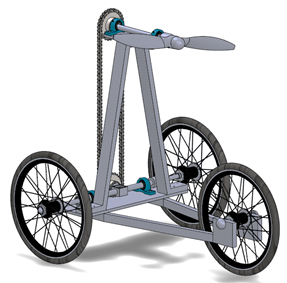
\includegraphics[width=\linewidth]{images/part9/drivetrainIter1.png}
%     \caption{Vehicle Iteration 1}
%     \label{fig:dtIter11}
% \end{wrapfigure}

\begin{figure}[!htbp]
    \centering
    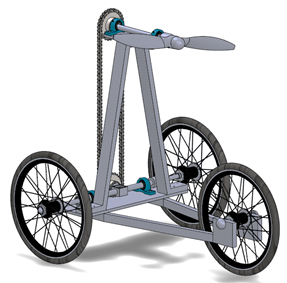
\includegraphics{images/part9/drivetrainIter1.png}
    \caption{Vehicle Iteration 1}
    \label{fig:dtIter1}
\end{figure}

In this iteration, the wheel choice, sprocket size choice, and propeller design were completed, along with the chain tensioner mechanism design. The axle was positioned underneath the bottom plate, to allow the structural members to be easily attached above via bolts. The chain tensioner allows tension to be applied to the chain during testing to prevent it from derailing. The propeller and the chain drive are situated on either side of the A-frame, which provides solid support via two pillow block bearings. Connections for the wheels were finalised to utilize the existing hubs on the wheels, with the front wheel being mounted via a small front fork manufactured from 6 mm aluminium plates, fixed onto the existing front axle. The rear wheels were mounted to the axle threaded at both sides, by nuts clamping the existing hubs (bearings removed) to the axle, locking the rotation.

Making the strut beams modular whilst achieving sufficient structural rigidity meant that the beams could not be directly welded onto the rear base plate that held the rear axle in place. To achieve this, a set of aluminium brackets were made by cutting sheet metal using a water jet cutter and welding them together at the specific angle required. The bottom brackets were made from 4 mm aluminium and the top bracket with 3mm aluminium. To supplement the brackets, a pair of aluminium blocks made with a CNC were made. These would be bolted together with the sheet metal brackets and help support the 20x40mm aluminium bars in compression load on each side. The design of these blocks were kept simple with minimal curvature to decrease the time of manufacture. During the assembly process, however, it was found that the sheet metal brackets were sufficiently strong to hold loads and therefore it was decided to not use them for testing.

A new iteration of the design was manufactured successfully for the preliminary wind tunnel test. During the test without the propeller attached, it experienced resonance due to non-concentric wheels causing a forced vibration which caused the A-frame to resonate, as explained in the "Resonance analysis" section. The problems due to this were addressed in iteration three of the design, where minor changes were made to the vehicle design before the 2nd wind tunnel test.

\begin{figure}[!htbp]
    \centering
    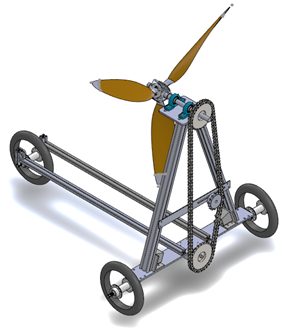
\includegraphics{images/part9/drivetrainIter2.png}
    \caption{Vehicle Iteration 2}
    \label{fig:dtIter2}
\end{figure}

Iteration 3 implements the design changes due to the resonance found in the initial testing of the vehicle. From combined analyses of test footage and simulations through the finite element analysis shown in the following section, it was found that fixing the propeller mount to the front wheel would likely decrease oscillations. It was decided that a strut must be placed between the top of the A-frame and the front wheel. This was done by adding an extra 20x20 mm strut member and this was connected using a separate set of custom brackets similar to the ones used to connect the A-frame to the rear base plate and top propeller mount plate.

\begin{figure}[!htbp]
    \centering
    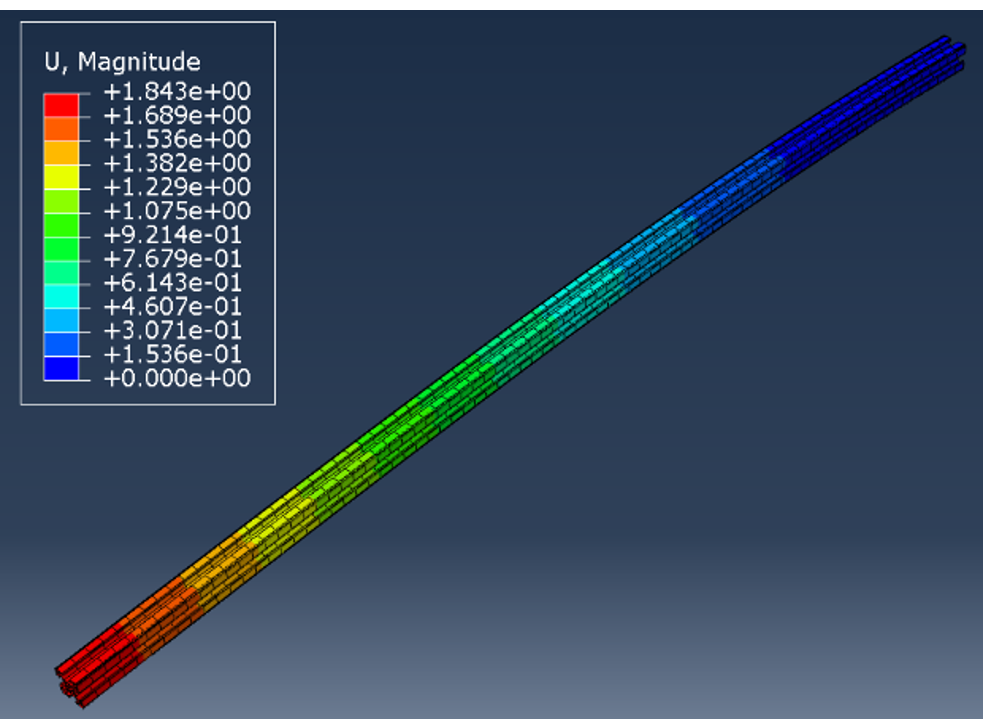
\includegraphics[width=0.5\linewidth]{images/part8/stucturethingy.png}
    \caption{FEA simulation showing the deformation of an aluminium profile beam under a $5\mathbf{kN}$ concentrated load}
    \label{fig:structhingy}
\end{figure}

\subsection{Manufacturing}
\begin{table}[!htbp]
    \centering
    \caption{Material properties}
    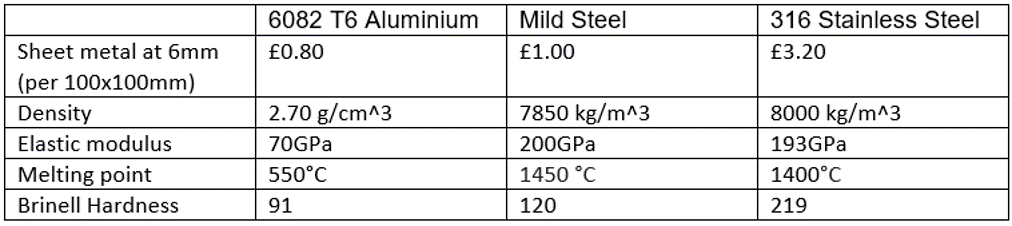
\includegraphics[width = \linewidth]{images/part8/materials.png}
    \label{tab:materials}
\end{table}

Table \ref{tab:materials} displays the generic material properties of the three sheet metals available in the EDMC. Within the project it was important to keep within the budget, therefore the main factor for this decision was the cost of the material. For the 6mm plate, the aluminium was the cheapest option and had the benefit of the lowest density and therefore weight. It was understood that the metal had a lower elastic modulus and hardness, but reducing the costs and weight were the main priorities, leading us to a decision of Aluminium.

The profile of the bar that was used in the experiment depended on two main factors: the deformation and the availability. Simple FEA analysis was conducted into the deformation characteristics of all the bar profiles, taking note of second moments of area and applying a uniform load. The FEA model was conducted under a simple Eulerian format which would induce the simplest deformation. The simple linear elastic model was applied in ABACUS and was applied to a model with the same length.


From the table of results, it’s clear that the I beam performs the best out of all the different beams when a point load is applied at one end. This demonstrates how this beam has the best directionality vertically than the other beams. The square beam also performs relatively well when tasked with deformation and has the benefit of having multiple directions of stability. The aluminium profile bar was modelled differently from the other bar types due to the complex nature of the bar profile. Inputting a DXF file into ABACUS I modelled the bar as a solid profile and deformed the structure. The deformation values were higher for the aluminium profile beam, but this was due to the limited computational cost availability. With more cell accuracy the deformation would drop significantly and gain a value much more similar to the I beam than is seen. With the aluminium profile, there are specific companies specialising in providing metal services. Bars can be pre-cut to specific lengths and less pressure will be put on connecting as the bars can be connected through the brackets that are also available on the websites. To increase the modularity of the vehicle, the best option would be to go for the aluminium profile to increase the modularity of the vehicle and project.

\subsection{Resonance analysis}

Before the completion of the vehicle, several wind tunnel tests were run without the propeller. This was useful in gauging approximate efficiencies of the wheels, gearbox, and drivetrain. As part of these tests, the moving ground was run between 0-10 m/s. It was observed that at around 3.5 m/s a resonance was set up in the A-frame (5.5 Hz) that yielded the vehicle very unstable to the point that a partial redesign would be necessary. The primary source of the energy input appeared to be the wheels which produced a driving frequency of twice their revolutions per second. This led to deriving a moving ground velocity – natural frequency relationship that would help to improve the vehicle’s stability:

\begin{equation}
V=\frac{f_{n} \times \pi D_{w h e e l}}{2} \approx 0.64 f_{n} m
\label{eq:natfreq}
\end{equation}

Thus, by increasing the natural frequency of the A-frame, which is effectively an inverted pendulum, the moving ground velocity for resonance to occur can be strategically placed much higher than the tested. A second improvement would be a stiffened A-frame that would oscillate with much lower amplitudes during resonance.

For validation, subsequent studies were made using SolidWorks frequency analysis using a simplified model of the vehicle shown in Figure \ref{fig:freqStudy}, where red regions represent the areas of highest deflection. The results showed that its mode 1 resonant frequency was 6.48 Hz (Corresponding to a rolling road speed of 4.14 m/s). This is slightly higher than observed in the wind tunnel but is likely down to real-world damping from unmodelled vehicle components. It is however similar enough for further testing.

\begin{figure}[!htbp]
    \centering
    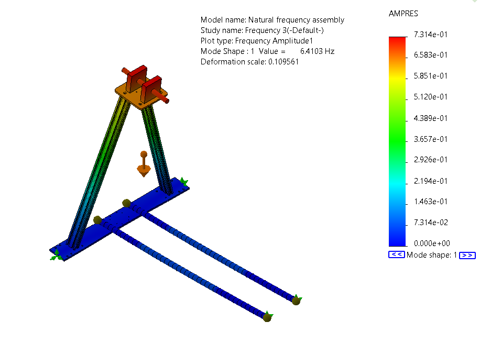
\includegraphics{images/part8/freqStudy.png}
    \caption{SolidWorks frequency study of vehicle}
    \label{fig:freqStudy}
\end{figure}

Three potential modifications were tested to assess their impact on the natural frequency of the vehicle:

\begin{itemize}
  \item A cross-beam structural member connecting top of A-frame to front of vehicle
  \item Larger plate at base of vehicle
  \item Thicker chassis members (increase second moment of area)
\end{itemize}

Performing SolidWorks frequency analysis on these variations (Figure \ref{fig:freqStudy2}) found that the latter two options did not sufficiently increase the natural frequency of the A-frame (12.2 Hz and 7.8 Hz respectively). Whilst their relative deflections were smaller, they do not entirely solve the problem of pushing resonance away from the operating speeds of the vehicle in the wind tunnel. The cross-beam option however was very effective, placing the natural frequency at around 76.8 Hz corresponding to a rolling road speed of 49.2 m/s. This design change would be critical but require moving the prop from the front of the A-frame to the back.

\begin{figure}[!htbp]
    \centering
    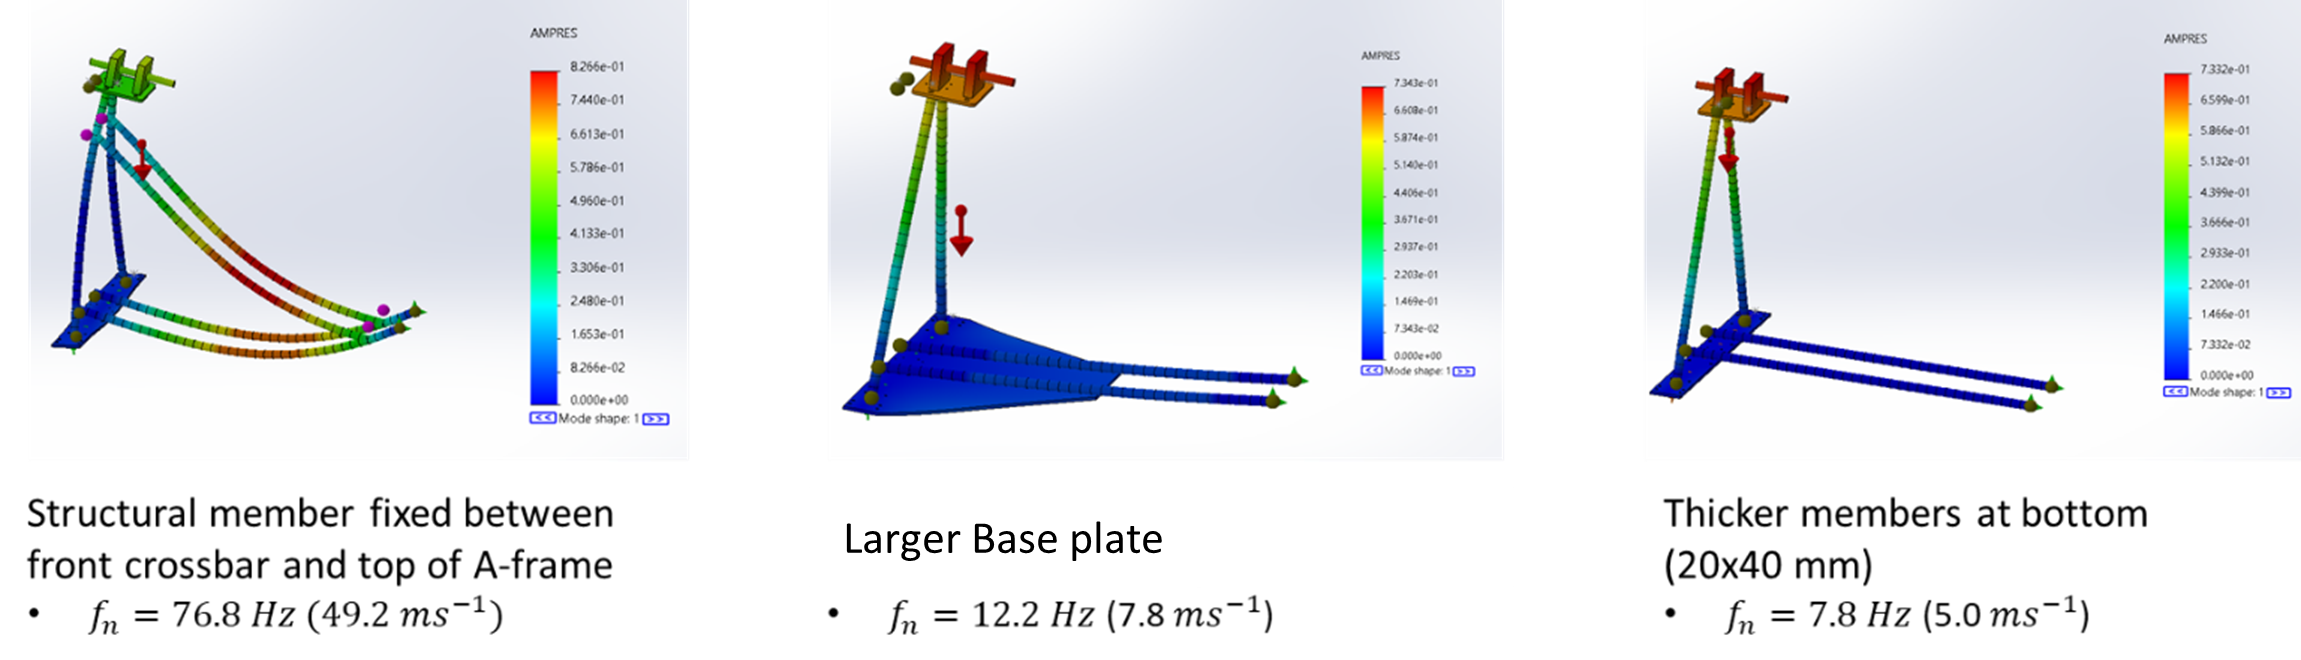
\includegraphics{images/part8/freqStudy2.png}
    \caption{Frequncy study of vehicle improvements}
    \label{fig:freqStudy2}
\end{figure}

\subsection{Structural update and vehicle reconfiguration}

This updated design takes into account the changes made due to the problems mentioned in the above section. To solve this, a 20x20 aluminium profile was fixed between the top of the A-frame and the front crossbar, and represents iteration three of the structure. This meant that the chain drive, propeller, and chain tensioner needed to be mirrored about the A-frame, which was a simple task due to the symmetry of the design. This allowed sufficient space for the supporting profile to be fitted effectively. It also meant that the propeller operated in a pusher configuration. The implications of this reconfiguration on propeller efficiency was not assessed further as the flow would likely be minimally affected by the this change.

\begin{figure}[!htbp]
    \centering
    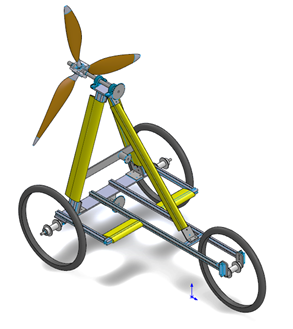
\includegraphics{images/part9/drivetrainIter3.png}
    \caption{Vehicle Iteration 3}
    \label{fig:dtIter3}
\end{figure}

\subsection{Aerodynamic streamlining}

Due to the jagged geometry of the aluminium extrusions used for the structure, an attempt was made to partially streamline the members ahead of the propeller for a potential improvement in performance. The design for this was made using a NACA 0030 aerofoil cross-section (The largest thickness to chord ratio plottable) wrapped around each beam. Two variations were made for the 20x20  mm and 20x40 mm bars (Figure \ref{fig:fairing3}), extending the 'width' of the beams by a mere 3 mm and 5 mm respectively. 3D printing was once again the go to option for manufacture, as the geometries could be produced quickly. Due to the lack of strength required for these parts, they could be printed using a single wall and no infill, and with the inclusion of a slot in the trailing edge could be opened and placed around the bar. These fairings were placed on several beams ahead of the propeller, however, time constraints and an increased focus on propeller manufacture meant that not all sections could be covered.

\begin{figure}[!htbp]
    \centering
    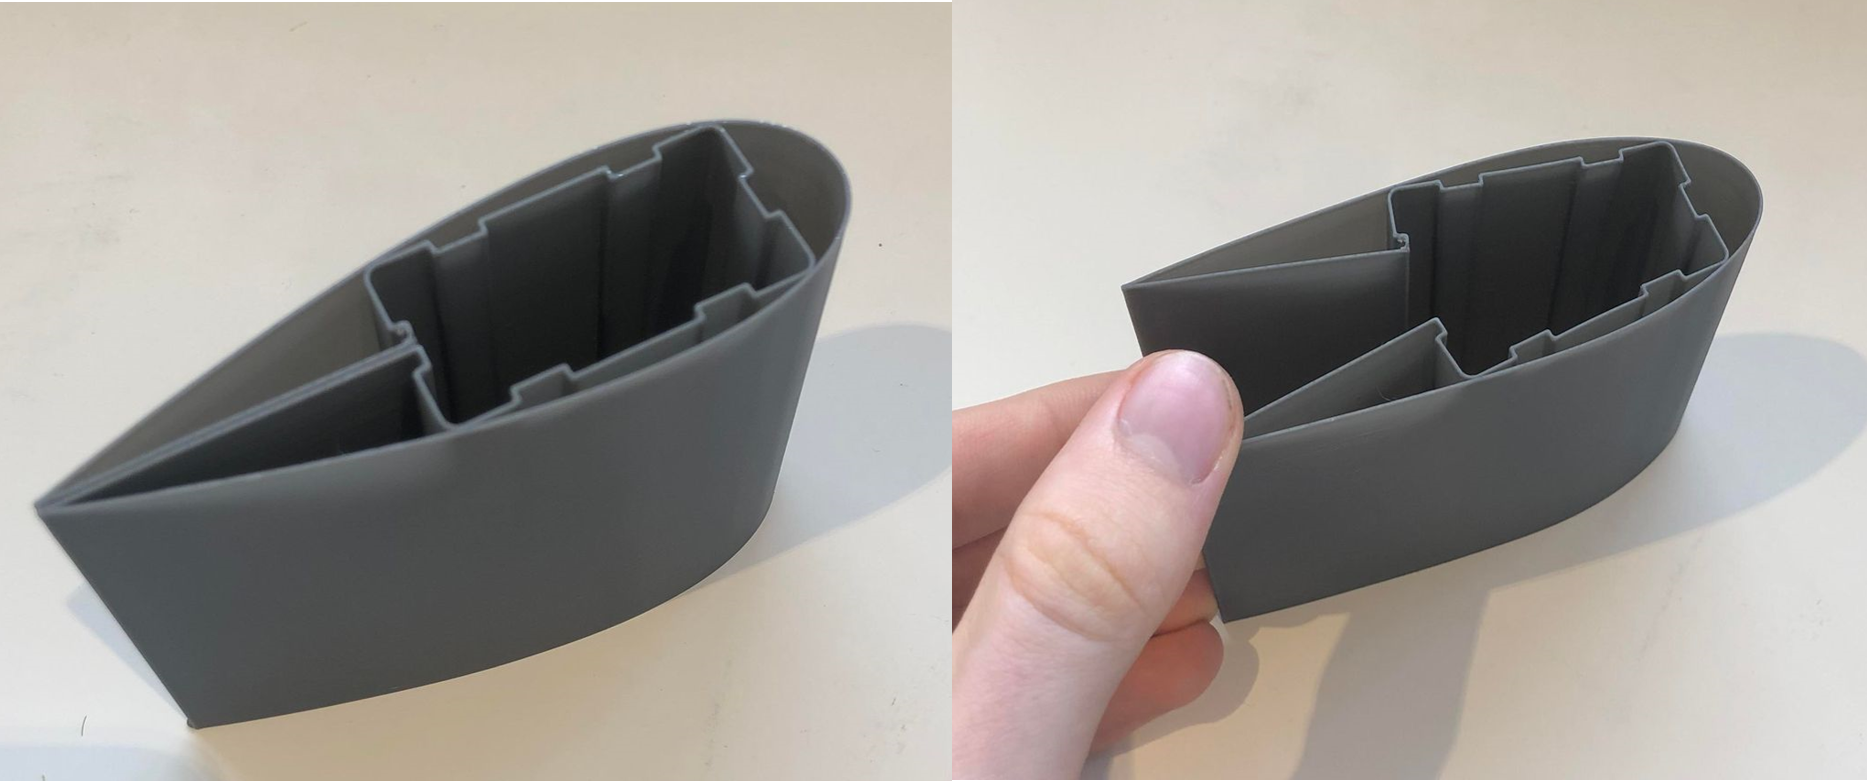
\includegraphics{images/part8/fairing3.png}
    \caption{3D printed fairing for aluminium extrusions}
    \label{fig:fairing3}
\end{figure}


\section{Drivetrain}

The drivetrain of the vehicle is fundamental in the transmission of torque between the wheels and the propeller. A key feature of this type of vehicle and a reason why it functions in the way it does is due to the way the wheels are geared to the propeller. Therefore, for the vehicle to be a valid test model, it must have a well designed, reliable and efficient drivetrain to link to the torque of the wheels to the propeller, and for the gear ratio to be correct to ensure that the propellers RPM is in the desired range for a given ground speed.

The design of the drivetrain is primarily driven by the need to maximise efficiency and ensure limited torque loss between the wheels and propeller. Resistance in the drivetrain directly contributes to vehicle drag which thrust from the propeller must overcome. In minimizing this resistance, producing a positive net thrust on the vehicle becomes more readily achievable. The drivetrain should preferably be simple in design to minimize the number of components, reducing weight which leads to lower rolling resistance and reducing the likelihood of mechanical failures during testing.

\subsection{Design Process and early concepts}

The design process was to consider a range of drivetrain concepts applied to the basic vehicle requirements for a propeller to be mounted to provide thrust, geared to the wheels. The different types of drivetrain system available were considered, and then a concept was developed after selecting the best choice. The drivetrain was designed in close tandem with the structure, due to the need for them to be well integrated. Figures \ref{fig:dtIter1}, \ref{fig:dtIter2} and \ref{fig:dtIter3} show how the vehicle was developed and iterated as further design decisions were made throughout the duration of the project, in response to factors such as availability of parts, cost, simplicity of design, ease of manufacture, and unforeseen problems arising in either manufacture or testing.

The primary design challenge faced for the drivetrain is transmitting torque between 2 shafts (wheel axle and propeller) aligned at 90-degrees to each other. To achieve this, the wheel axle required a 90-degree gearbox to transfer wheel axle torque to an axle either orthogonal or parallel to the propeller shaft above. The secondary challenge of linking this gearbox output to the propeller was then considered. Practical options included using a vertical transmission shaft, chain drive, or belt drive.

\begin{figure}[!htbp]
    \centering
    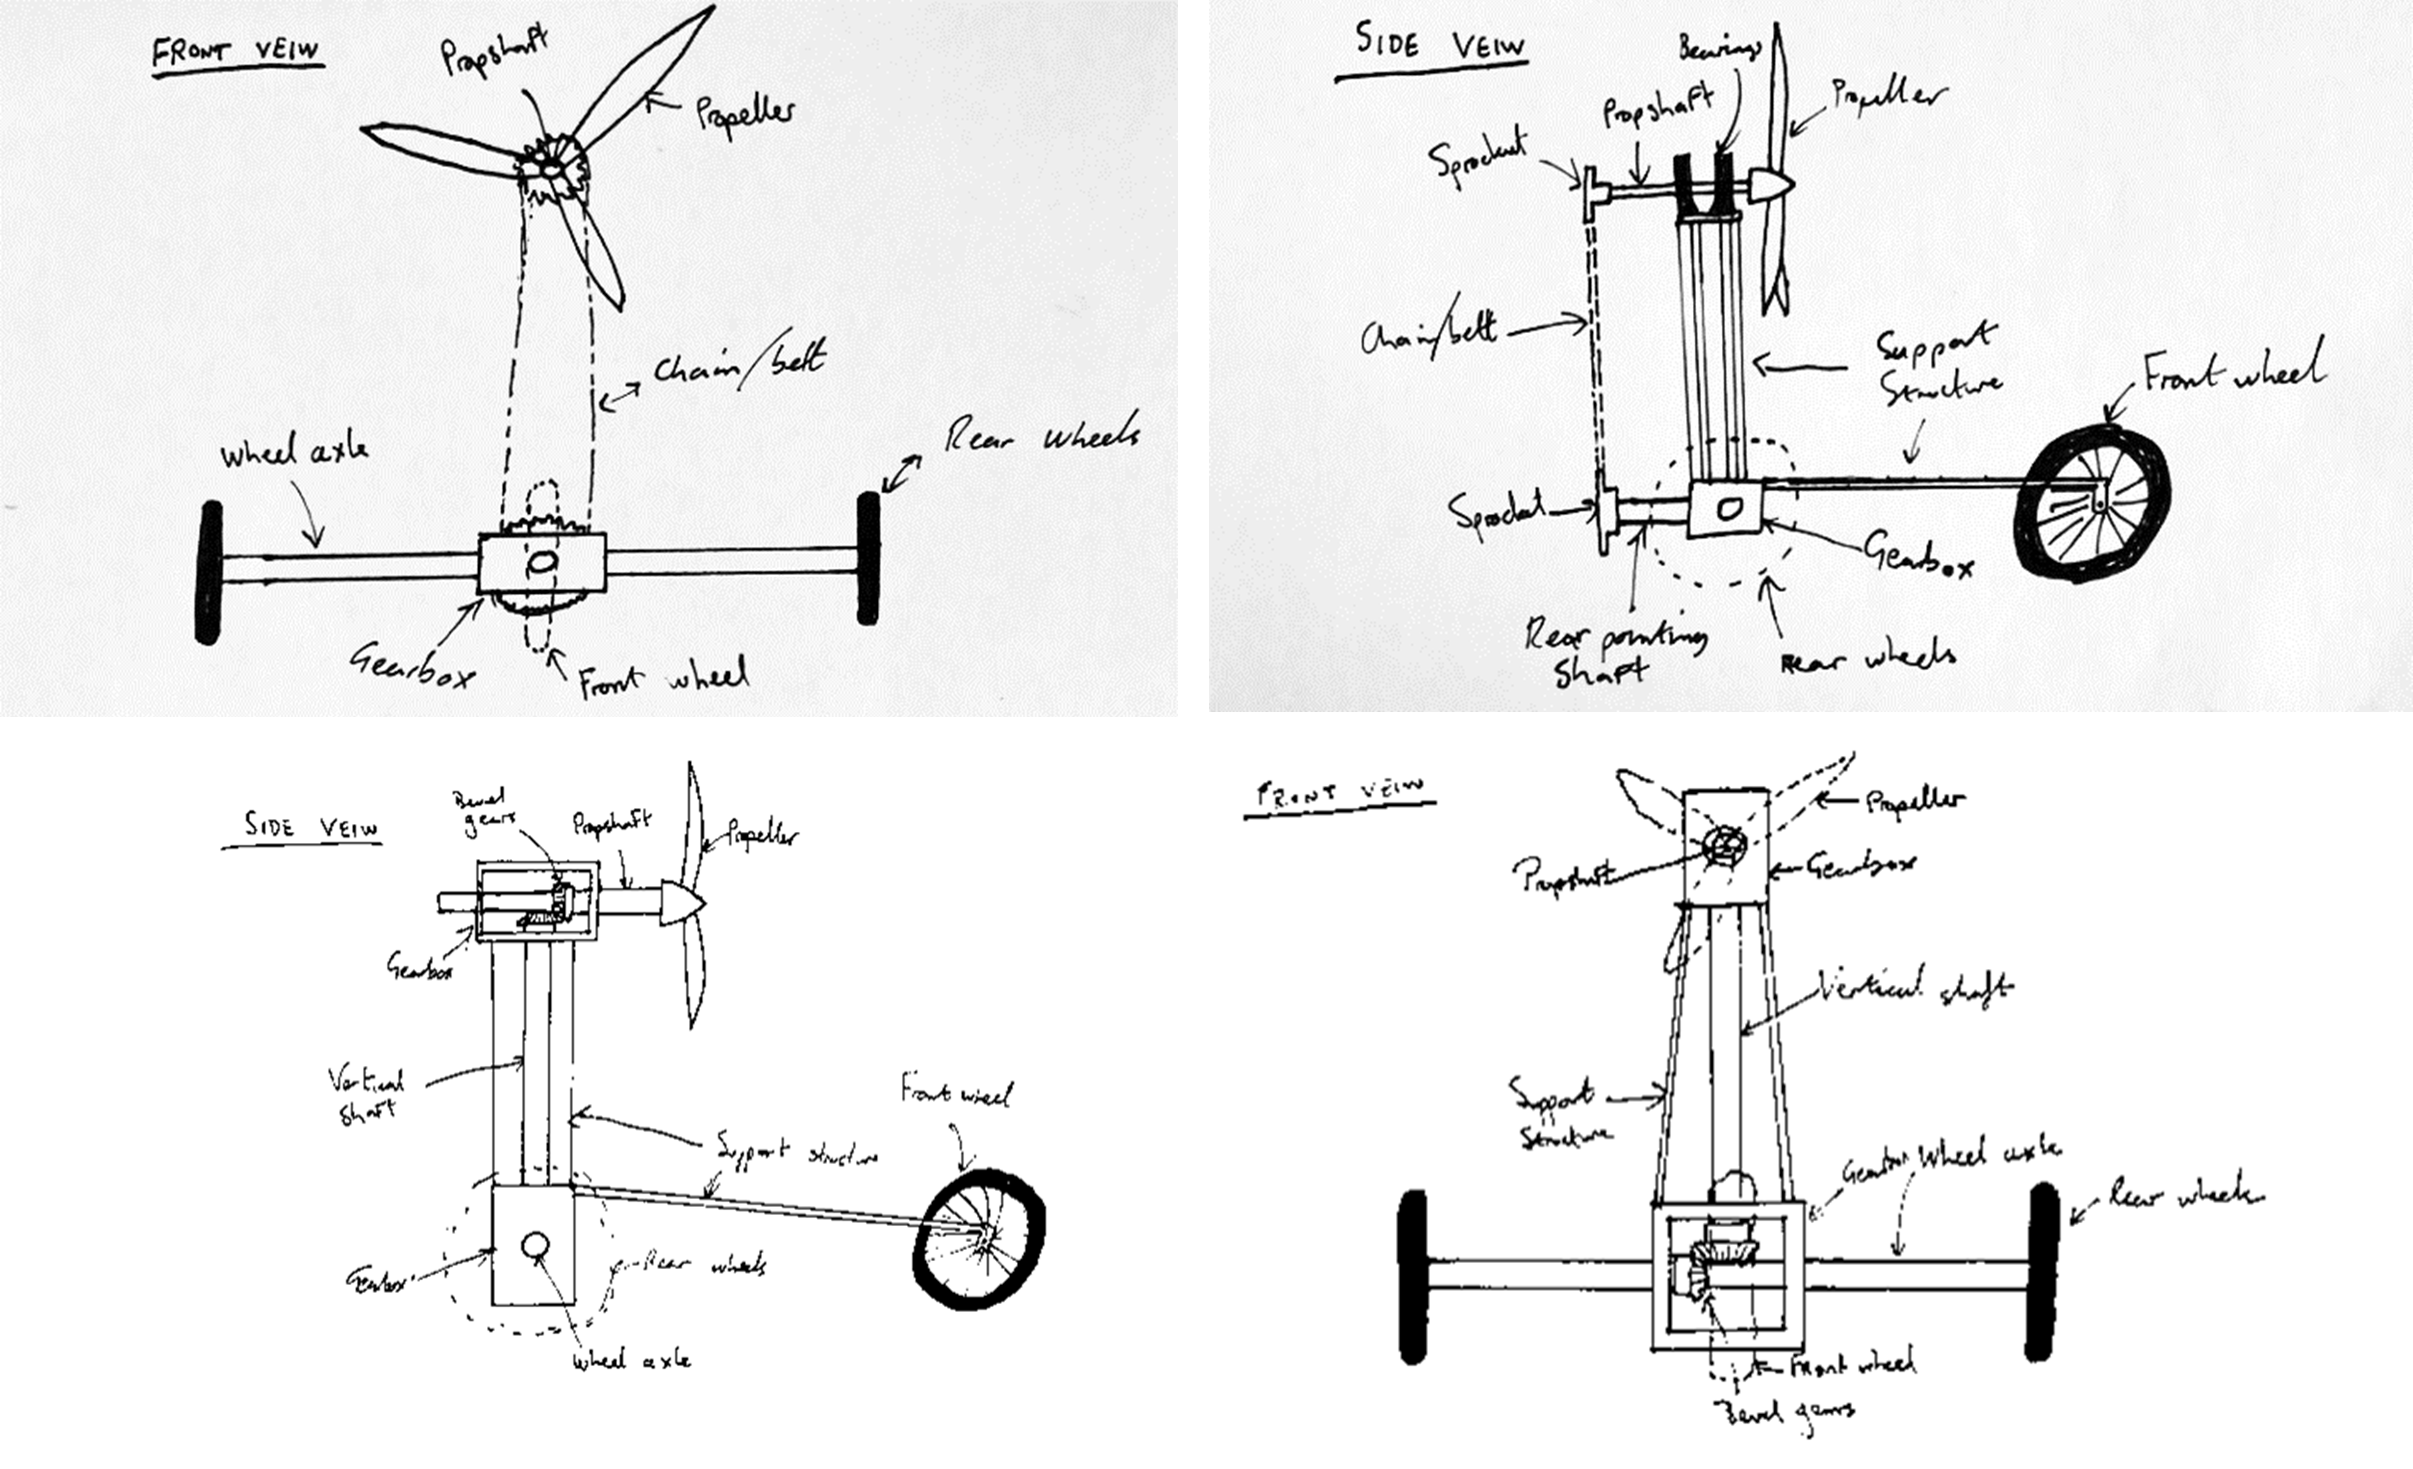
\includegraphics{images/part9/drivetrainSketches.png}
    \caption{Sketches of drivetrain}
    \label{fig:dtsketches}
\end{figure}

% Please add the following required packages to your document preamble:
% \usepackage[table,xcdraw]{xcolor}
% If you use beamer only pass "xcolor=table" option, i.e. \documentclass[xcolor=table]{beamer}
\begin{table}[!htb]
\caption{Drivetrain system choice considerations}
\label{tab:drivetrainChoices}
\centering
\begin{tabular}{|
>{\columncolor[HTML]{\CellColor}}l |p{4cm}|p{4cm}|p{4cm}|}
\hline
\textbf{Type of drivetrain}      & \cellcolor[HTML]{\CellColor}\textbf{Shaft}                                                                                                                       & \cellcolor[HTML]{\CellColor}\textbf{Chain}                                                                     & \cellcolor[HTML]{\CellColor}\textbf{Belt}                                                                                                                    \\ \hline
\textbf{Cost   considerations}   & Shafts come with a cost due to the   amount of material used, often hardened to withstand high torques. Would   require two gearboxes which increases the cost & Chain drive components are cheap with a large range of gear ratios and chain sizes.                        & Belt components are more expensive than chain components. The length of the belt is unchangeable once purchased, assuming the right length can be found. \\ \hline
\textbf{Availability   of parts} & Readily available, variety of   sizes. Limited gearbox options online however                                                                                & Easily acquired, especially for small chain pitches for compact chain drives not coping with high torques. & Rarer than chain parts, difficult to acquire correct sizes.                                                                                              \\ \hline
\textbf{Complexity}              & Simple with minimal interacting   parts                                                                                                                      & Medium complexity, would require tensioner mechanism.                                                      & Would require specialist cogs which run the belt, and a way of applying tension.                                                                         \\ \hline
\textbf{Efficiency}              & High due to small number of   interacting parts, namely 2 bevel gears and shaft bearings on the gearbox                                                      & Losses due to friction between the sprockets and chain.                                                    & Losses due to the elasticity of the belt.                                                                                                                \\ \hline
\textbf{Modularity}              & Only allows for one gear ratio to   be used                                                                                                                  & Allows for sprockets to be changed to alter the gear ratio between tests.                                  & Difficult to adjust or change gear ratios due to high tension.                                                                                           \\ \hline
\textbf{Potential   problems}    & Bevel gears would wear easily if   the shafts were not perfectly aligned, any vibrations could lead to failure   and are difficult to change                 & Vibrations can occur leading to inefficiency and the chain detaching from sprockets during testing.        & The length of the belt is unchangeable once purchased, assuming the right length can be found.                                                           \\ \hline
\end{tabular}
\end{table}

Based on these considerations, the chain drive design was chosen due to the desire to change sprocket sizes and adjust the gear ratio, which can be easily achieved with a chain. Off-the-shelf components for this purpose are less readily available for belt systems. The pure shaft drive would eliminate the possibility of changing gear ratios altogether without a major redesign.
Of all the options, the chain drive design is relatively simple, and the positioning of the two shafts means the chain can be aligned very close to the gearbox and the pylon, reducing stresses in the system when under tension.

\subsection{Chain Tensioner Mechanism}

It was necessary to keep the chain in tension during tests to prevent derailment. This was achieved with a smaller sprocket running on a bearing positioned on a slotted plate about 1/3 of the way up the vehicle A-frame, which could be moved left or right along the slot to apply/remove tension in the chain. A bolt running through the sprocket was used to keep it fixed to the plate.

Figure \ref{fig:tensionerFinal} shows the final chain tensioner mechanism used for the 2nd wind tunnel test. The sprocket has 24-tooth with a bearing custom fitted in the borehole. A series of washers and spacers ensure the sprocket is aligned with the chain, and the two nuts lock the clamping force on the system while the sprocket is allowed to spin freely on the bearing. A secondary safety bolt is fixed in the slot next to the mechanism to prevent tension from releasing during the tests. This final design came about after the first wind tunnel test, which outlined problems with the first design. Initially, as shown in Figure \ref{fig:tensionerInitial}, a 16-tooth sprocket was used, which ran using 3D printed PLA spacers. This worked reasonably well for low ground speed tests, but at ground speeds exceeding 8m/s, the high friction between the sprocket and spacers generated enough heat to soften the PLA (glass transition phase), causing a reduction in clamping force in the tensioner bolt, and loss in the tension of the chain as the tensioner began to move. This led to chain de-railing and potential damage risks to the vehicle/wind tunnel. The 2nd design in Figure \ref{fig:tensionerFinal} eliminated this problem and tension was successfully kept in the chain throughout the tests at all ground speeds after this.

\begin{figure}[!htbp]
    \centering
    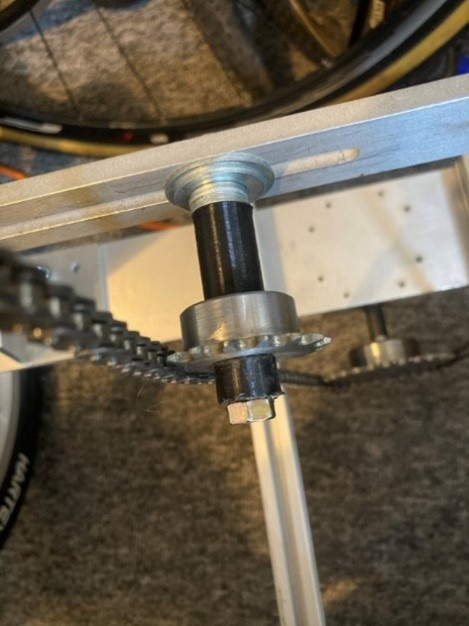
\includegraphics{images/part9/chainTensionerInitial.jpg}
    \caption{Initial chain tensioner mechanism}
    \label{fig:tensionerInitial}
\end{figure}

\begin{figure}[!htbp]
    \centering
    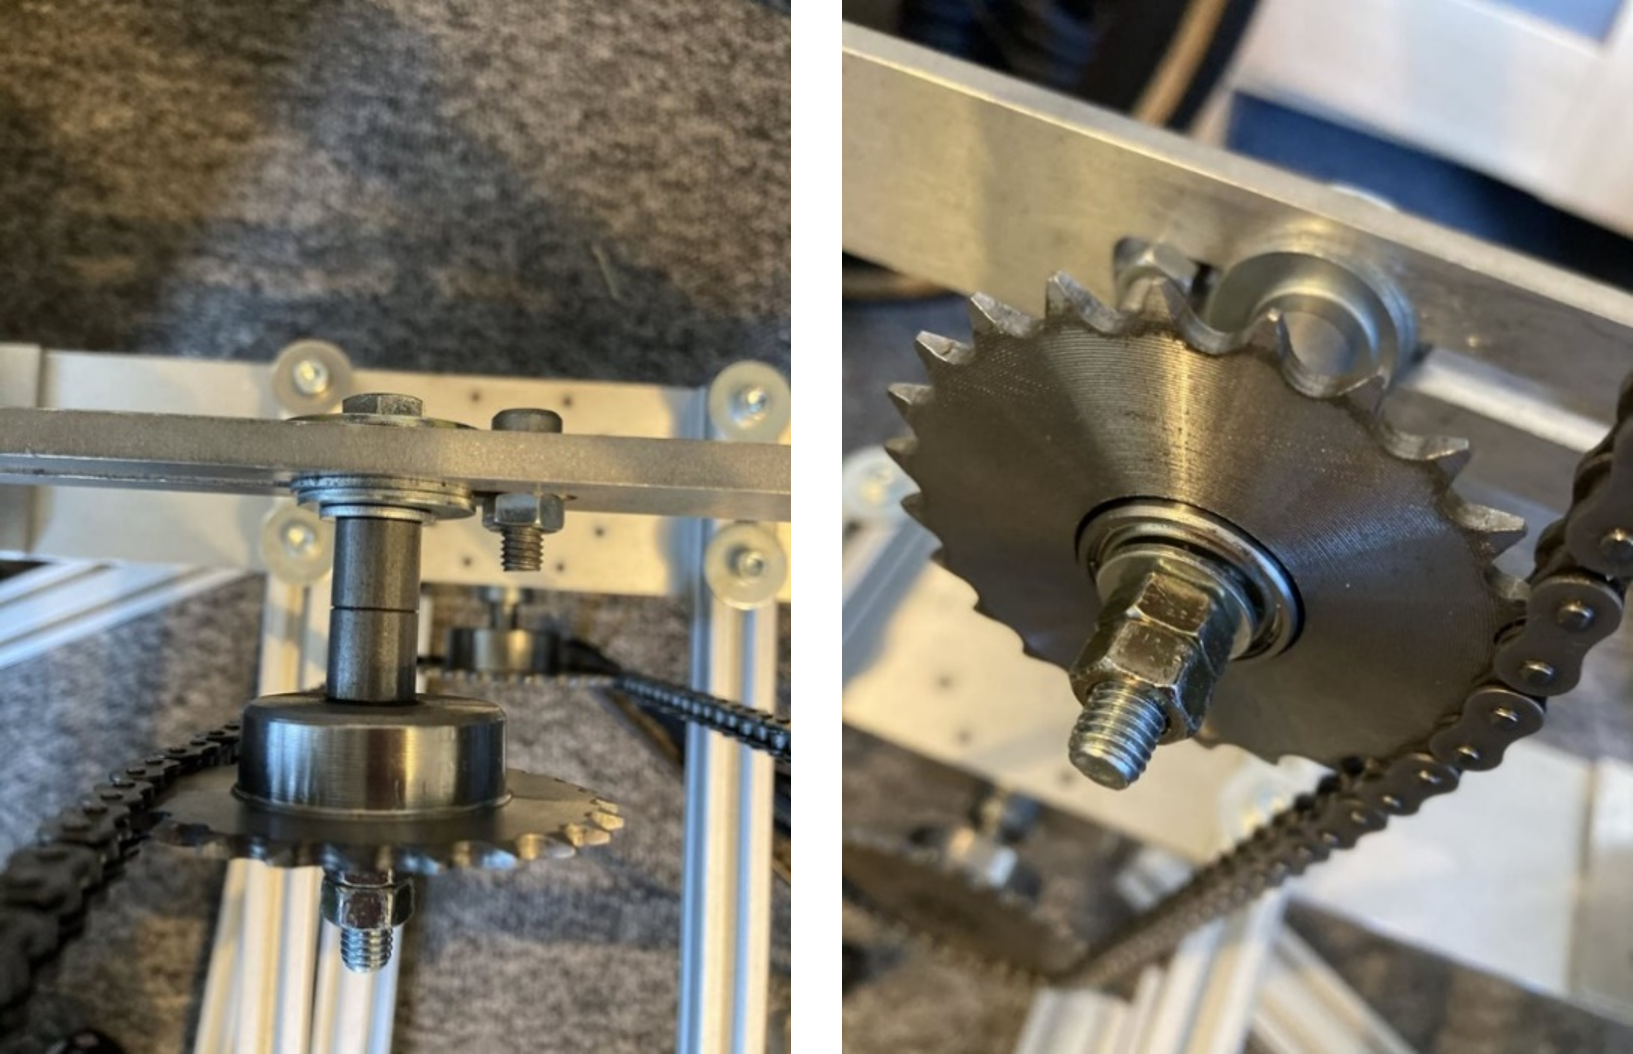
\includegraphics{images/part9/chainTensionerFinal.png}
    \caption{Final chain tensioner mechanism}
    \label{fig:tensionerFinal}
\end{figure}

\subsection{Axle and wheels}

The choice of axle diameter for gearbox input and output was 10 mm. For the torques experienced, it is more than wide enough to limit bending and very unlikely to fail. The initial material choice was hardened stainless steel, which was changed to mild steel due to the need to thread the ends for attachment to the wheels. This was not possible with hardened steel due to its high hardness.

\begin{figure}[!htbp]
    \centering
    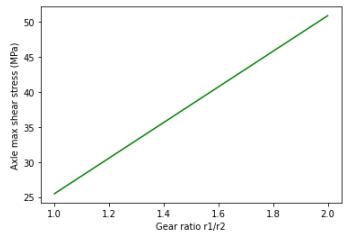
\includegraphics{images/part9/axleStress.png}
    \caption{Maximum shear stress experienced by the rear driven axle as the gear ratio between the sprockets is increased}
    \label{fig:axleStress}
\end{figure}

The maximum shear stress rating for Low Carbon steel is 350 MPa, which is significantly higher than the predicted maximum stresses on the steel axle used on the vehicle. This means the axle has very virtually no risk of failure. The combination of pillow bearings and gearbox bearings pin the axle at various points, evenly distributing the loads from the structure on the axle, which minimises the potential for rotational bending.

\begin{figure}[!htbp]
    \centering
    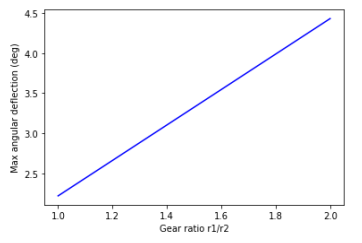
\includegraphics{images/part9/axleDeflection.png}
    \caption{Maximum shear deflection in the axle as gear ratio is increased}
    \label{fig:axleDeflection}
\end{figure}

Figure \ref{fig:axleDeflection} shows the maximum angular deflection for the given maximum torque for each gear ratio is shown. It remains low even at the high gear ratio of 2. This justifies the use of a 10mm steel axle as a lightweight solution, operating well within the parameters in Figures \ref{fig:axleStress} and \ref{fig:axleDeflection}.

The two choices for wheels were metal-spoked bike wheels with a narrow width, for low rolling resistance, or wooden wheels manufactured using laser cut plywood, which would have a rubber band/belt fitted to the circumference to provide traction and damping. Bike wheels with tires containing inner tubes would provide greater damping than the wooden wheels. The decision was made to use off-the-shelf bicycle wheels due to their quality and lightness with a low relative cost. The size of the wheels was determined based on the gear ratio requirements between the angular velocity of the wheels and the propeller.


Figure \ref{fig:propRPM} shows that for a variety of gear ratios, the output RPM of the propeller is not hugely affected by a change in the wheel diameter, ranging here from 14 to 19 inches. Therefore, the choice of wheel size is not hugely driven by the diameter, and a sensible size can be selected based on the vehicle size, market availability and cost considerations.

\begin{figure}[!htbp]
    \centering
    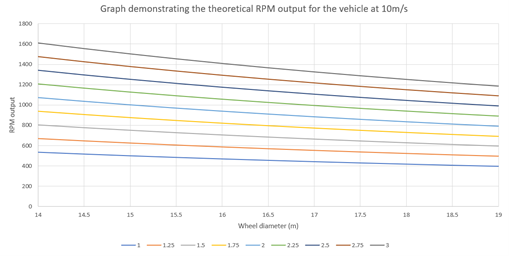
\includegraphics{images/part9/propRPM.png}
    \caption{Propeller RPM vs. wheel diameter for a range of gear ratios}
    \label{fig:propRPM}
\end{figure}

The vehicle was fitted with 16-inch diameter wheels, which were the cheapest and most readily available option. This also was an appropriate size for the wind tunnel, so the load cell wheel mounts could be attached at an appropriate height above the ground, almost level with the wheel hubs. Also, using 16-inch wheels meant the gear ratio used between the two sprockets could be 1:1, as the desired propeller RPM was 470 when the ground speed was 10m/s.

The metal spoked bicycle wheels selected could be easily attached to the 10mm shaft centrally due to the hub design allowing them to be clamped via bolts on the threaded ends of the shaft.

\begin{figure}[!htbp]
    \centering
    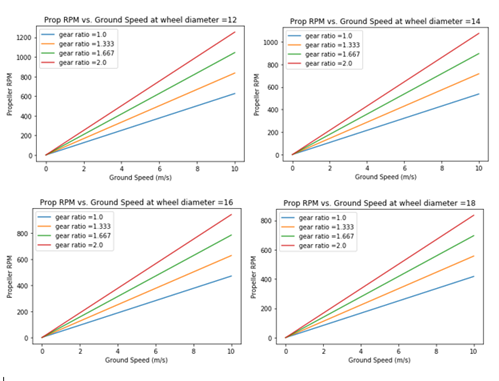
\includegraphics[width = 0.7\linewidth]{images/part9/propRPM2.png}
    \caption{Propeller RPM vs. moving ground speed for a range of gear ratios and wheel diameters (inches)}
    \label{fig:propRPM2}
\end{figure}

Figure \ref{fig:propRPM2} shows that for a wheel diameter of 16 inches, the ground speed of 10m/s, the propeller RPM is 470 when the gear ratio between the lower and upper sprocket is 1, which is the speed to the propeller was designed to operate most effectively at.

Figure \ref{fig:rollResistance} demonstrates how rolling resistance increases with a reduction in wheel radius. With the minimal wheel numbers on the vehicle, the importance of ensuring a minimal rolling resistance can be seen by the large increases in rolling resistances at lower wheel radius values. This was a large consideration when deciding on the wheel radius with the largest diameter possible being selected to minimize this quantity. Furthermore, the 16-inch diameter chosen for the wheels was mainly set by the wind tunnel load cell mounts and their ability to hold the vehicle in place. Reducing the wheel radius from this value was thought to increase the vehicle's rolling resistance, especially with the vehicle size in comparison to the wheels.

\begin{figure}[!htbp]
    \centering
    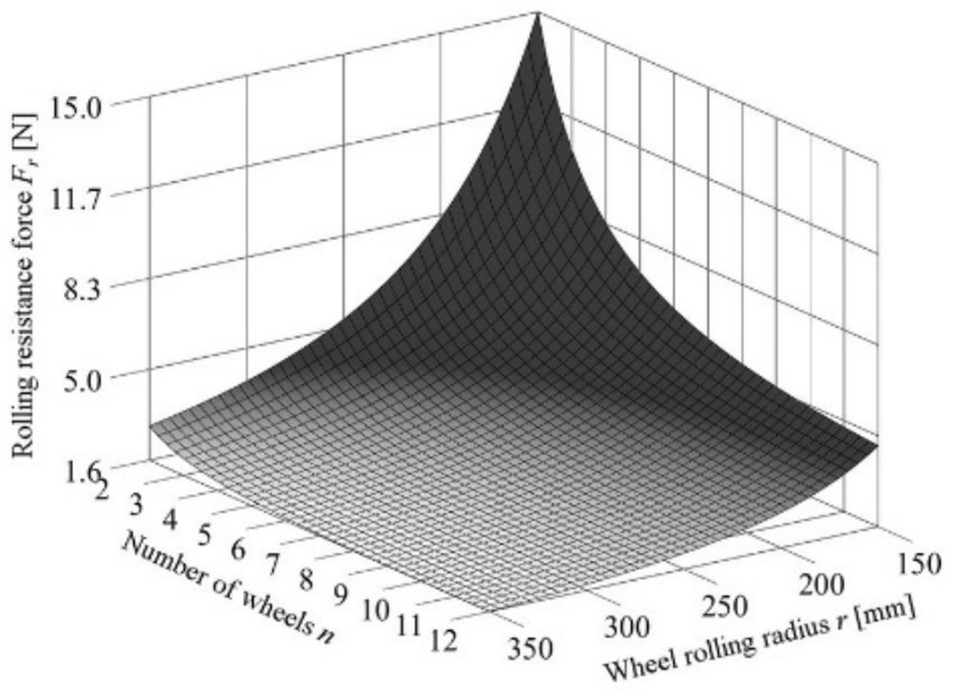
\includegraphics{images/part9/rollingResistance.jpg}
    \caption{Propeller RPM vs. moving ground speed for a range of gear ratios and wheel diameters (inches) \cite{Baldissera}}
    \label{fig:rollResistance}
\end{figure}

\subsection{Gearing and bearings}

A 1:1 gear ratio right angle gearbox was used, which has an aluminium body and stainless-steel bevel gears, which attach via grub screws to 10mm axles aligned at 90-degrees to each other.

For the sprockets, hardened stainless steel Simplex bore sprockets were used, which had an 8mm pitch, so a small, light chain could be used as the torques experienced are low in the drivetrain, with an estimated maximum of 5 Nm.

% Please add the following required packages to your document preamble:
% \usepackage[table,xcdraw]{xcolor}
% If you use beamer only pass "xcolor=table" option, i.e. \documentclass[xcolor=table]{beamer}
\begin{table}[H]
\caption{Gearbox transmission types}
\label{tab:gearboxComp}
\centering
\begin{tabular}{|
>{\columncolor[HTML]{\CellColor}}l |p{6cm}|p{6cm}|}
\hline
\textbf{Gear type}       & \cellcolor[HTML]{\CellColor}\textbf{Advantage}                                                               & \cellcolor[HTML]{\CellColor}\textbf{Disadvantage}                                                          \\ \hline
\textbf{Helical}         & \begin{tabular}[c]{@{}l@{}}Runs smoothly.\\ Can be mounted parallel and straight.\end{tabular}           & \begin{tabular}[c]{@{}l@{}}Must select same handed gears.\\ Power losses due to slippage.\end{tabular} \\ \hline
\textbf{Bevel}           & \begin{tabular}[c]{@{}l@{}}Good slipping resistance.\\ Can easily change a 90 degree angle.\end{tabular} & Prone to noise effects.                                                                                \\ \hline
\textbf{Rack and pinion} & Straight line pitch circle.                                                                              & Rotary to straight line.                                                                               \\ \hline
\textbf{Spiral bevel}    & \begin{tabular}[c]{@{}l@{}}Good noise resistance.\\ Can easily change a 90 degree angle.\end{tabular}    & Prone to slipping.                                                                                     \\ \hline
\end{tabular}
\end{table}

From Table \ref{tab:gearboxComp}, it’s clear to see that the bevel and mitre gearing options were the best two options for gearing the drivetrain gearbox at the centre of the axle rod. The straight-lined bevel gearing is more widely available for general purchase than the mitre option, it was therefore decided that the vehicle would have bevel gears for the gearbox.


% Please add the following required packages to your document preamble:
% \usepackage{multirow}
% \usepackage[table,xcdraw]{xcolor}
% If you use beamer only pass "xcolor=table" option, i.e. \documentclass[xcolor=table]{beamer}
\begin{table}[H]
\caption{Comparison of the different bearing options available}
\label{tab:bearingsComp}
\centering
\begin{tabular}{|m{2.5cm} |l|m{9cm}|}
\hline
\cellcolor[HTML]{\CellColor}\textbf{Type}                    & \cellcolor[HTML]{\CellColor}\textbf{Cost} & \cellcolor[HTML]{\CellColor}\textbf{Additional} \\ \hline
\textbf{Pillow bearing}          &                                       &                                             \\
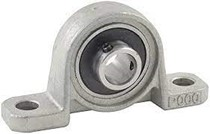
\includegraphics[width=\linewidth]{images/part9/bearing1.jpg}                              & \multirow{-2}{*}{£9.29}               & \multirow{-2}{\linewidth}{Bearing insert aligns with grub screw. Cost effective and light. Comes with clearance holes to increase modularity.}                    \\ \hline
\textbf{Deep grove ball bearing} &                                       &                                             \\
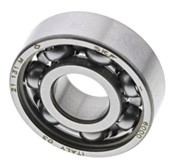
\includegraphics[width=\linewidth]{images/part9/bearing2.jpg}                               & \multirow{-2}{*}{£2.39}               & \multirow{-2}{\linewidth}{Would need welding to a section of the main structure. Cost effective and light.}                     \\ \hline
\textbf{Bolt oval housing}       &                                       &                                             \\
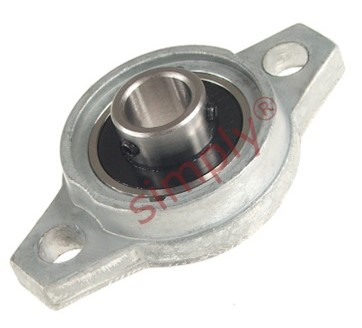
\includegraphics[width=\linewidth]{images/part9/bearing3.jpg}                              & \multirow{-2}{*}{£11.99}              & \multirow{-2}{\linewidth}{Bearing has two grub screws. Clearance holes would allow for modularity in the design. }                     \\ \hline
\end{tabular}
\end{table}

\begin{figure}[!htbp]
    \centering
    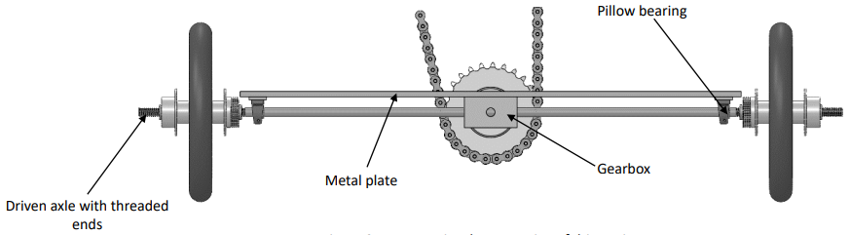
\includegraphics[width=\linewidth]{images/part9/drivetrainbackview.png}
    \caption{Back view of the drivetrain of the vehicle, highlighting the pillow bearing}
    \label{fig:drivetrainBackView}
\end{figure}

The connection between the axle rod and the main horizontal plate for the vehicle illustrated in Figure \ref{fig:drivetrainBackView} had the issue of having one component being in rotation and one component being still on the vehicle. Analysing the different options it was decided that the solution to this issue was using bearings as this would fix the axle rod and maintain the structural integrity of the vehicle. Comparing the different bearing options, Figure \ref{tab:bearingsComp} helped us realise that the pillow block bearing was the best option to complete this connection as this allowed easy connections to be made between the axle rod and the flat plate. The housed bearing offered additional benefits to the vehicle as the guide holes on the components helped increase the vehicle modularity, which would help during the testing of the vehicle if any configuration changes were needed.





\section{Pitch Control Mechanism and Hub}
After early studies of the vehicle and its parameters, it was found that the propeller blade pitch had a high impact on the performance of the propeller. Due to this vehicle’s peculiar operating conditions (the necessity to output highly efficient thrust over a wide range of RPMs), the best way to achieve this was to have the possibility of modulating the blade pitch. For this reason, a pitch variation mechanism was designed.

\subsection{Requirements}

Changing the pitch angle of the blades has an impact on the advance ratio of the propeller. The advance ratio is defined in Equation \ref{eq:advratio}, where $Z$ is the freestream velocity (in this case the relative velocity), $n$ the rotation speed of the propeller in $rad/s$ and $D_p$ the diameter of the propeller. It is shown in \cite{bronz2012multi} that the propeller efficiency varies along with the advance ratio. Figure \ref{fig:advratioeffi} displays the efficiency of different propellers as a function of the advance ratio.

\begin{figure}
    \centering
    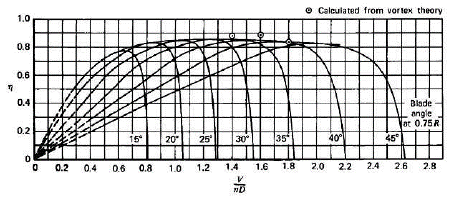
\includegraphics{images/part7/advanceratioeffi.png}
    \caption{Typical propeller efficiency curves as a function of advance ratio $J$ \cite{bronz2012multi}.}
    \label{fig:advratioeffi}
\end{figure}

\begin{equation}
    J = \frac{Z}{n D_p}
    \label{eq:advratio}
\end{equation}

Substituting the following definitions of the relative wind speed $Z$ and the rotational speed of the propeller $n$ which are specific to this case, one obtains Equation \ref{eq:advanceratiodw}, where $R_w$ is the radius of the wheels and $i$ the gear ratio.

\begin{equation}
    Z = V-W
    \label{eq:relativevel}
\end{equation}

\begin{equation}
    n = \frac{i V}{R_w}
    \label{eq:rpm}
\end{equation}

\begin{equation}
    J = \frac{V-W}{i V D_p}R_w
    \label{eq:advanceratiodw}
\end{equation}

Equation \ref{eq:advanceratiodw} illustrates that the advance ratio is not constant over the operational domain. This is also shown on Figure \ref{fig:advanceratios}. The advance ratio for this case is plotted for various gear ratios. Possessing the ability to vary the pitch of the propeller is therefore of great help in maximising the efficiency of the propeller and achieving the best results possible.

\begin{figure}
    \centering
    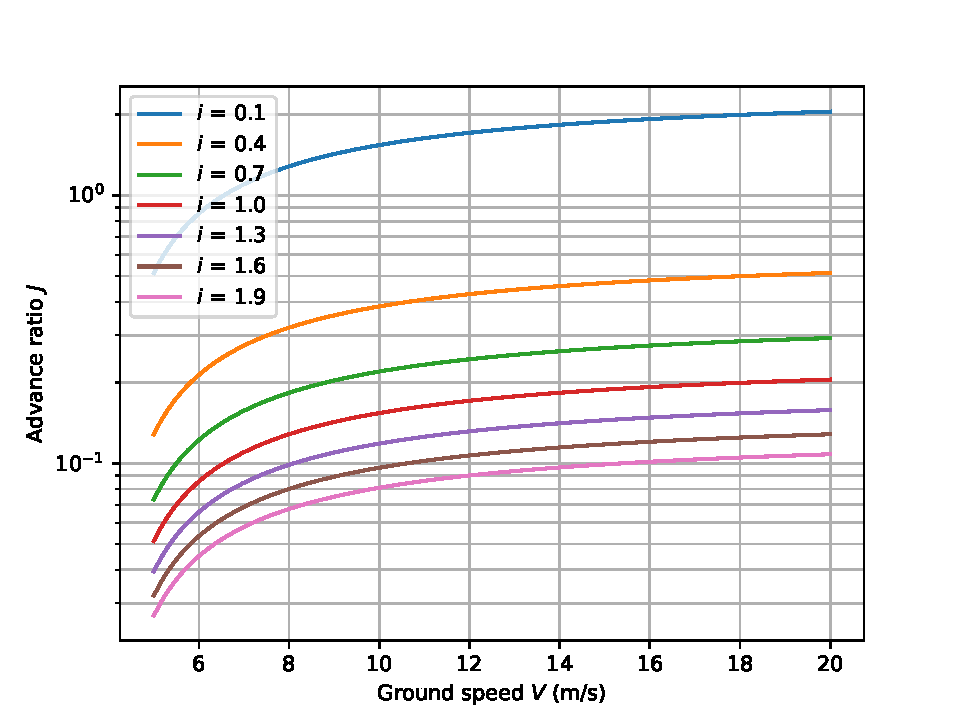
\includegraphics[width = 0.7\linewidth]{images/part7/advance ratios.pdf}
    \caption{Advance ratio as a function of ground speed. $i$ is the gear ratio. Values of $D_p$ and $R_w$ taken from the final design values. An arbitrary wind speed of $4\mathbf{m.s}^{-1}$ was taken.}
    \label{fig:advanceratios}
\end{figure}

The aim is to change the pitch angle of all propeller blades by the same amount, reliably, precisely, and easily so that it can be performed during the wind tunnel experiments without the risk of producing unbalanced thrust. The blades would need at least a pitch angle range of 30 degrees for it to be impactful.

The hub needed to fit and attach securely onto a 16mm diameter propeller shaft chosen due to its high polar moment of inertia, resulting in good torsional strength. It would be expected to spin at around 600 RPM, hence support the high centrifugal forces of the propeller blades, but also unscrew reasonably easy to change the configuration if needed.

\subsection{Design process}

Initially, a swash-plate mechanism similar to those seen on helicopters was studied. It simultaneously changes all blade angles. A motor would be used to slide a plate up and down to control the blade angle even whilst testing the vehicle in the wind tunnel. However, its intricacy was deemed too high for the design requirements set. Figure \ref{fig:swash} shows the initial design. Hence a simpler revision was created. Each blade was to be rotated individually and manually. Being a structurally important component, the hub was built in aluminium and stainless steel to be able to withstand far greater stresses than it would experience in testing. This also meant that the hub could be reusable for larger scale vehicle designs.

\begin{figure}[!htbp]
    \centering
    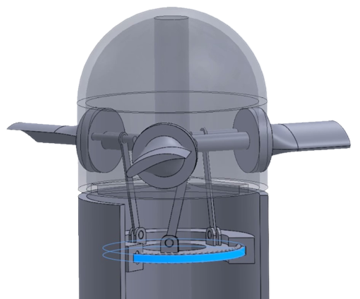
\includegraphics{images/part7/swash.png}
    \caption{Initial swash-plate-like hub design}
    \label{fig:swash}
\end{figure}

The first design iteration of the hub is shown in Figure \ref{fig:iter2}. It utilises a circular shape to fit the blades around the hub. An aluminium blade root is attached to the blade with three bolts, inserted in the main part of the hub, and can therefore be rotated for each blade, enabling a range of pitch angles of 30 degrees. This design could be modified easily to fit three blades as well. However, because of the circular shape of the faces connected to the blades, the overall diameter of the hub was too wide. Since the propeller diameter is constrained, it is important to minimize the size of the hub so that the blades can be longer and produce more thrust.

\begin{figure}[!htbp]
    \centering
    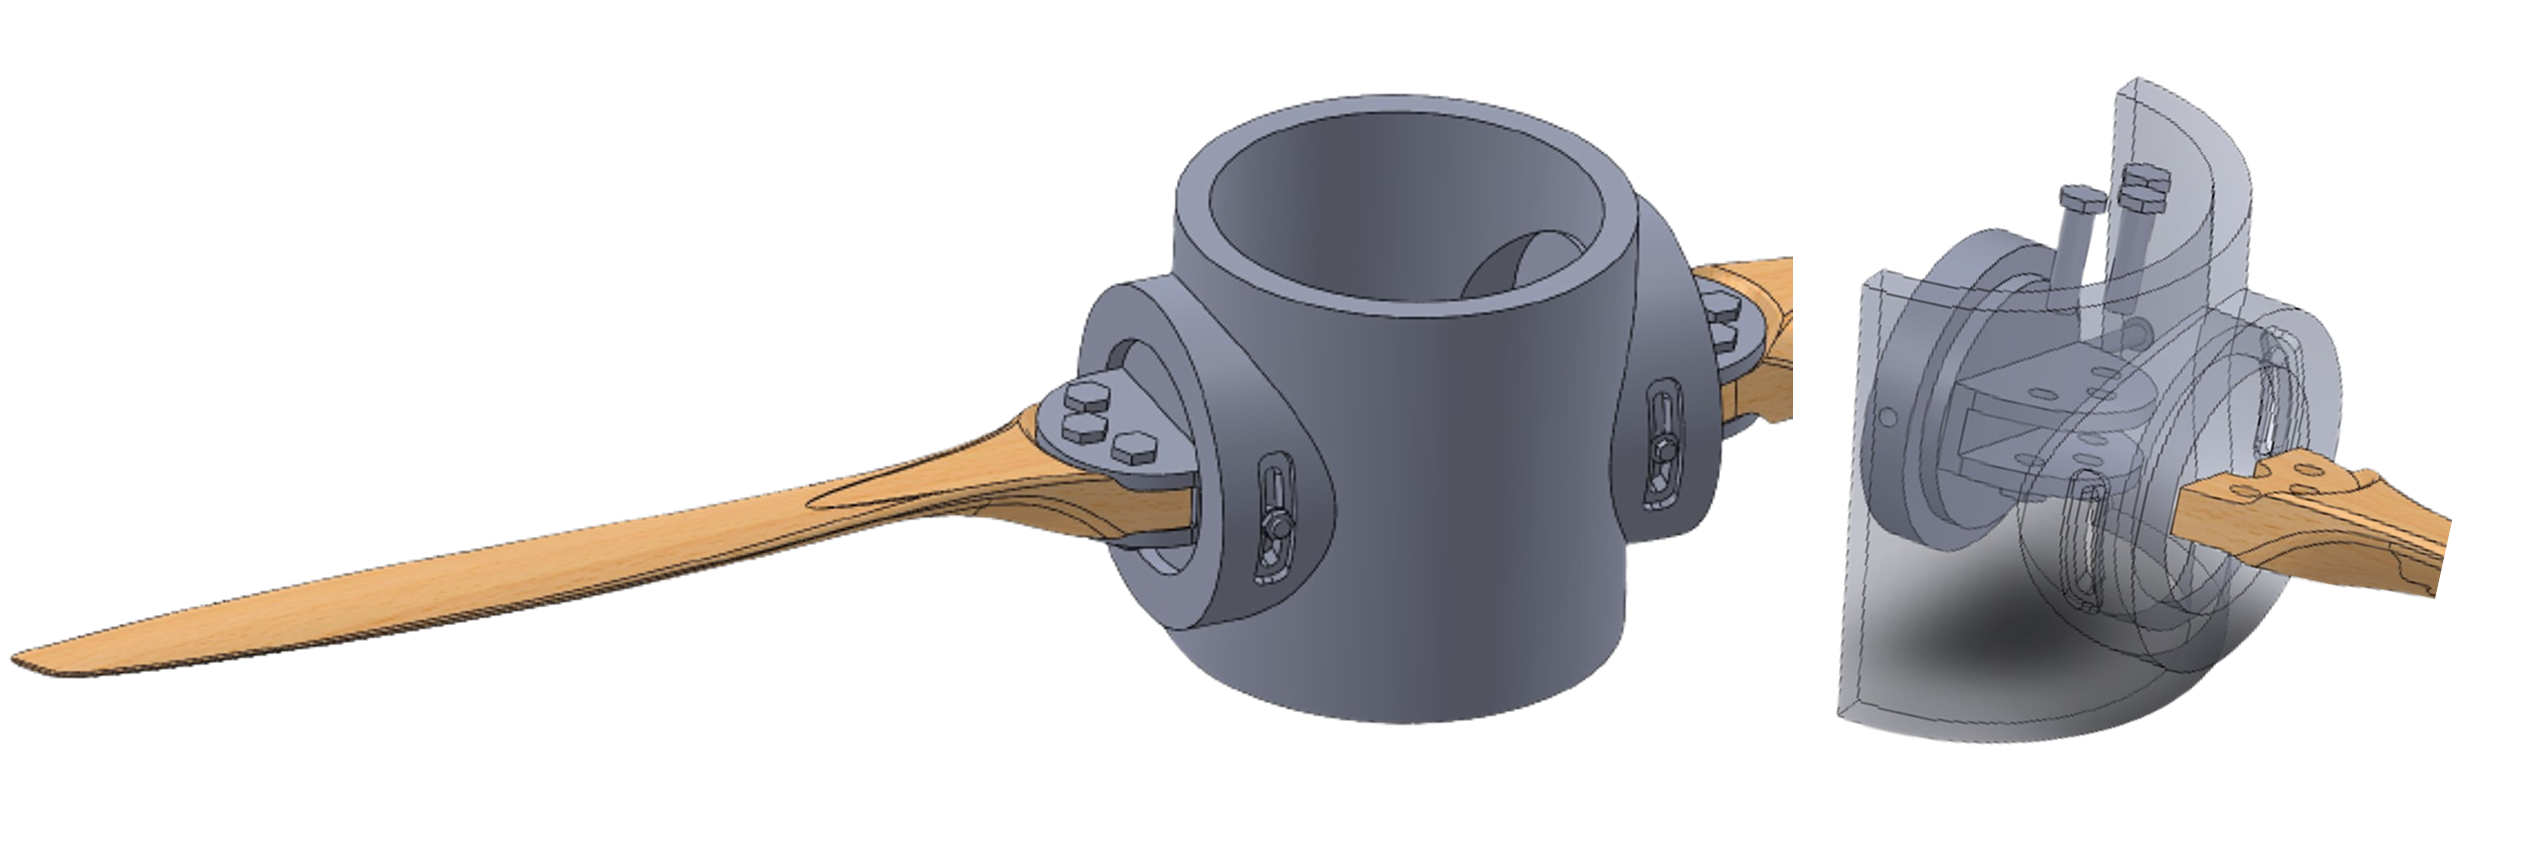
\includegraphics[width=\linewidth]{images/part7/iter2.png}
    \caption{Dual-blade circular hub design}
    \label{fig:iter2}
\end{figure}

\begin{figure}[!htbp]
    \centering
    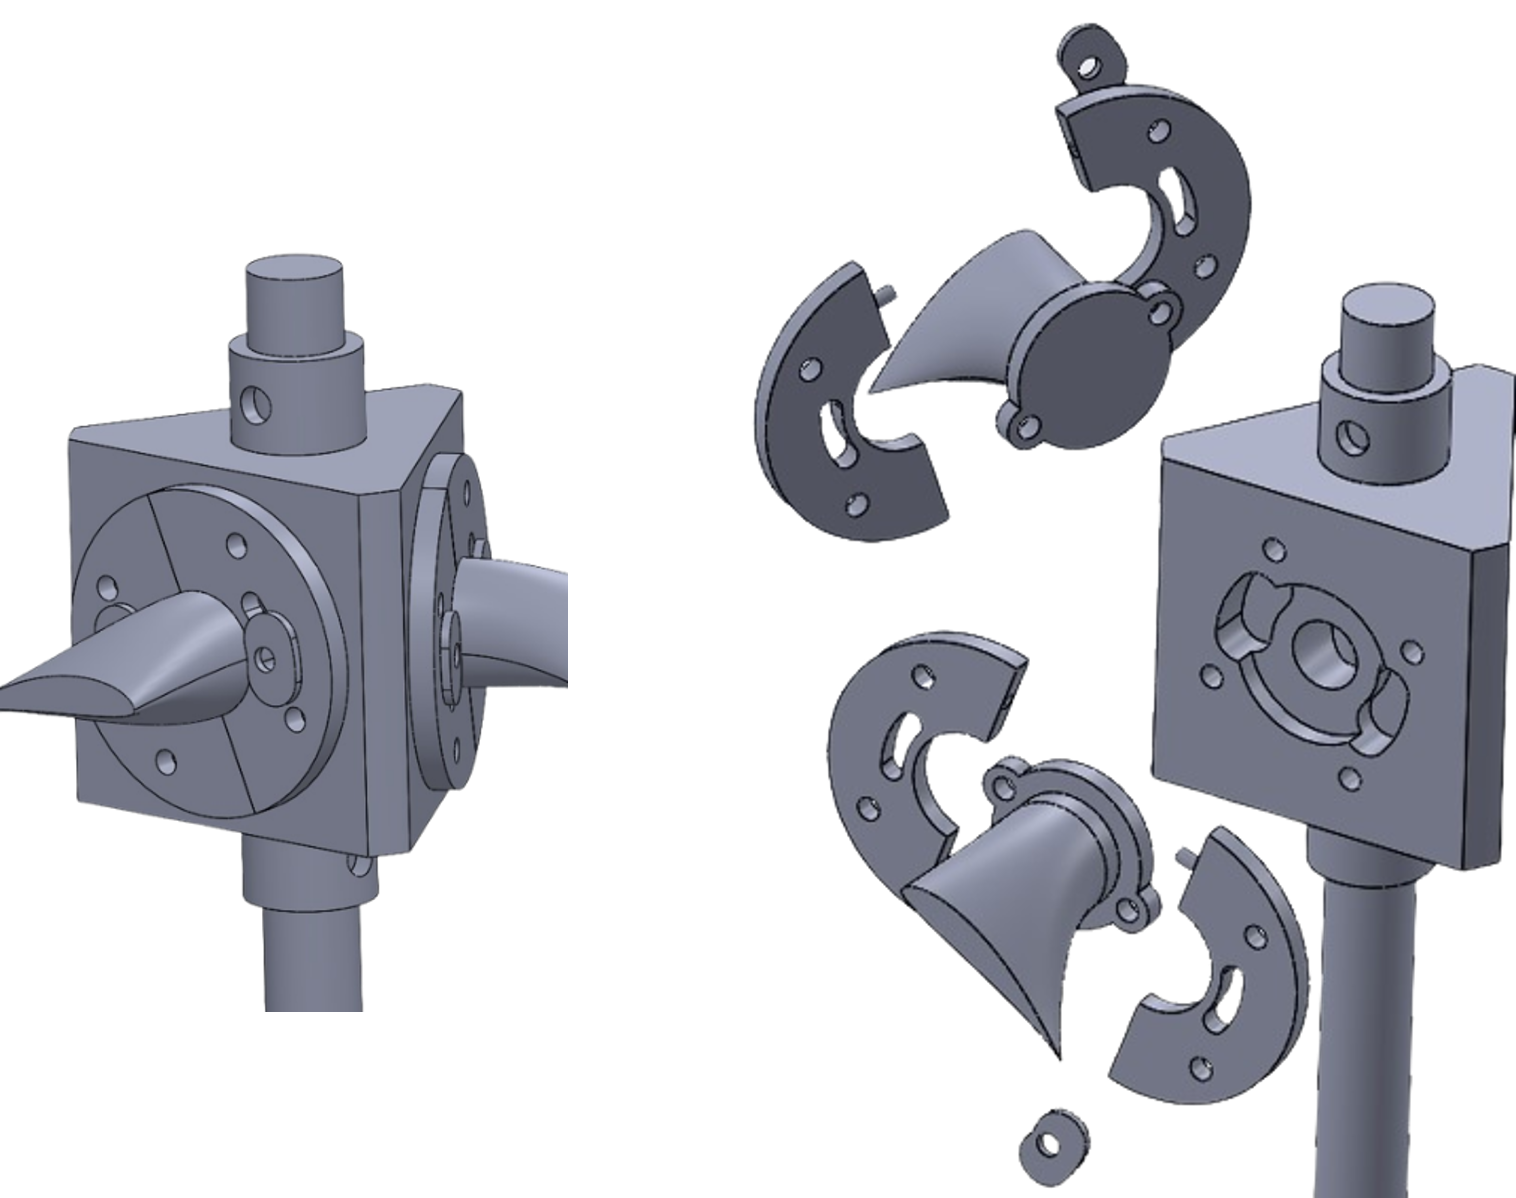
\includegraphics{images/part7/explodedhub.png}
    \caption{Collapsed and exploded view of the final hub design}
    \label{fig:explodedview}
\end{figure}

Therefore, for the second iteration shown in Figure \ref{fig:explodedview}, the shape was more triangular. With the faces on which the blades fix onto the hub being flat, this reduces the amount of excess material used and reduces the overall diameter of the hub. The diameter of the hub is only 71 mm. It consists of more separate pieces as can be seen on the exploded view in Figure \ref{fig:explodedview}, but is a lot more compact.

\subsection{Manufacturing}

Being a structurally important component, the hub was built in aluminium. The propeller can be reasonably expected to be able to spin at 600 RPM and withstand the necessary centrifugal forces of the blades, which has been estimated to be around 5.3 N per blade.

The hub was made by the EDMC and had to be designed to simplify the machining process, reducing the manufacturing cost of the part. The parts securing the blades to the hub were cut from a sheet of aluminium using a water-jet cutter.

\begin{figure}[tbp]
    \centering
    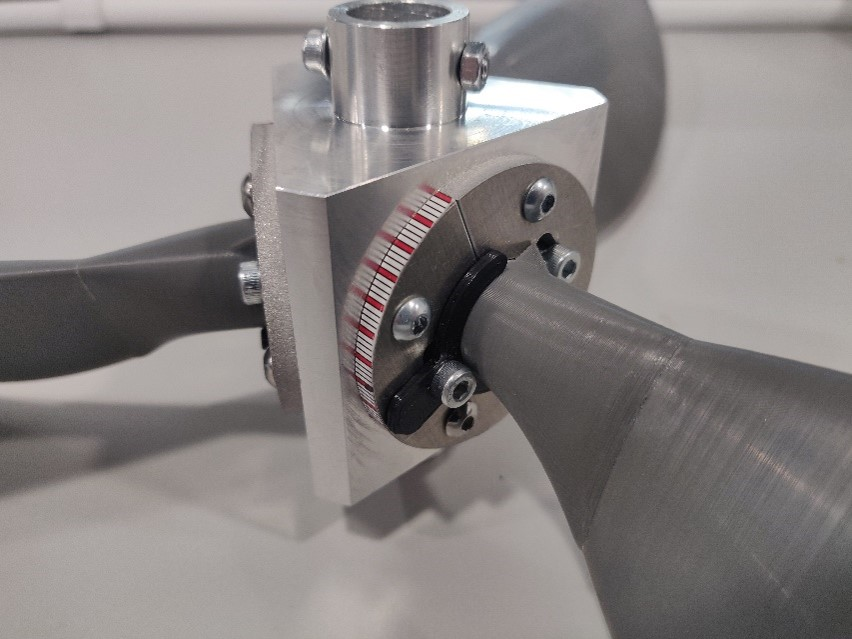
\includegraphics{images/part7/finalphoto.jpg}
    \caption{Final manufactured hub}
    \label{fig:finalhub}
\end{figure}


\section{Propeller}
The propeller was quickly identified as one of the key components of the vehicle. The first step in designing a propeller was to analyse its design requirements. Looking at Equation \ref{eq:e}, it was made clear that propeller efficiency needed maximising to achieve the greatest possible speeds. Therefore, adequate parameters to ensure this high efficiency had to be chosen. One of the better ways to achieve this is to build a model.

\subsection{Design process}

Several models exist for the theoretical analysis of propellers and fans in general. The two main ones are the disk actuator theory and blade element theory. Disk actuator theory was deemed too basic for this application as the aim was to generate and analyse various blade geometries. It is not possible with this model as it treats the fan as a disk through which a pressure change occurs. Therefore, blade element theory was chosen.

A Python script was written that could produce simple blade planforms using a finite number of cross-sections (typically around 10). The code integrated Xfoil to use accurate lift and drag coefficients of different aerofoils over various angles of attack. The script would maximise efficiency for each cross-section at a desired operating point of the vehicle and output pitch and chord length (based on desired thrust distribution) profiles along the blade. The propeller was then tested at varying wind and group speeds to determine its performance at different operating conditions as shown in Figure \ref{fig:jamesresults}, demonstrating a maximum efficiency of over 90\%. Issues with convergence and the inability to incorporate Reynold’s number limited the expected reliability of this code but made a good starting point.

\begin{figure}[!htbp]
    \centering
    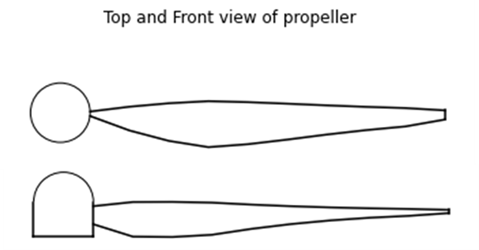
\includegraphics{images/part6/jamescode.png}
    \caption{Initial python script generated propeller profile}
    \label{fig:jamesprop}
\end{figure}
\begin{figure}[!htbp]
    \centering
    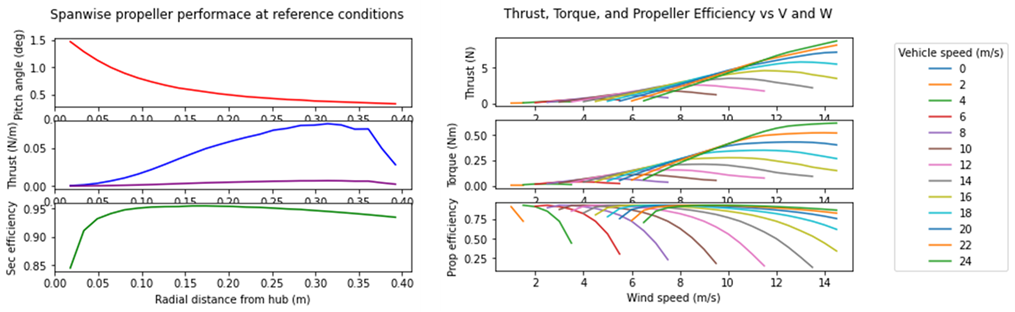
\includegraphics{images/part6/jamesresults.png}
    \caption{Performance of python-generated propeller blade at varying wind and ground speeds}
    \label{fig:jamesresults}
\end{figure}

In a second iteration, a new python script was written. The aim was to integrate JavaProp, a program that uses blade element theory. This code, developed by Martin Hepperle, had shown to produce satisfying results in generating blade geometries from inputs. It was also able to output their associated total force plot, and presented no issues with convergence. Testing demonstrated similarities between iterations 1 and 2 of the code, however, the latter was deemed more suitable due to the well-established reliability of JavaProp.

As shown in Figure \ref{fig:pyflowchart}, first, a set of parameters were defined for JavaProp to output the optimal propeller geometry for these conditions. Once the geometry was generated, it could then be tested by outputting the performance over the operational domain. Using the output, choosing the parameters was made easier. 

For the performance evaluation and to generate the plots shown in Figure \ref{fig:pythonresults}, it was required to integrate the equations defined in \cite{drela20dead}. The force of the wheels was obtained from the thrust generated by the propeller using Equation \ref{eq:fulleq}. Derivation for this equation is available in \cite{drela20dead}.

\begin{equation}
F_{n e t}=F_{p}\left\{1+\left[\frac{2 V \eta_{g} \eta_{v}}{(V-W)+\left((V-W)^{2}+\frac{2 F_{p}}{\rho A_{p}} \frac{1}{\eta_{\text{swirl }}}\right)^{\frac{1}{2}}}-1\right]^{-1}\right\}^{-1}
\label{eq:fulleq}
\end{equation}

Estimations were made for the different efficiency parameters. The overall propeller efficiency outputted by JavaProp was used for $\eta_p$ it was then used to compute the viscous efficiency $\eta_v$. For the swirl efficiency $\eta_{swirl}$, a conservative value of 0.95 was taken, as advised in \cite{drela20dead}. For the transmission efficiency $\eta_g$ a conservative value of 0.93 was taken after surveying common efficiency value ranges.

\begin{figure}[!htbp]
    \centering
    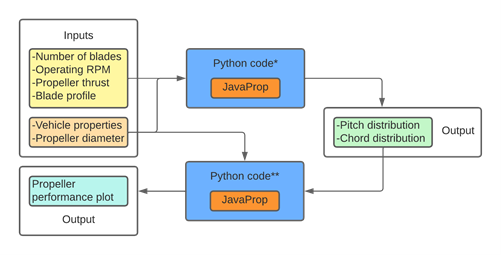
\includegraphics{images/part6/flowchart.png}
    \caption{DWFTTW theoretical model inputs and outputs. *Geometry generation from specific operating conditions. **Performance evaluation over various operating conditions}
    \label{fig:pyflowchart}
\end{figure}

Figure \ref{fig:pythonresults} shows how the performance of the propellers generated by JavaProp was evaluated. Force contours were plotted to study and better understand the various parameters of a propeller. It is important to note that blade element theory does not allow for zero inflow cases. This is the reason why the thrust estimated is 0 below the $\beta = 1$ line, as the relative wind is 0 or negative. The positive force zone outlines the domain in which the vehicle would theoretically be able to operate without the implication of any exterior forces.

\begin{figure}[!htbp]
    \centering
    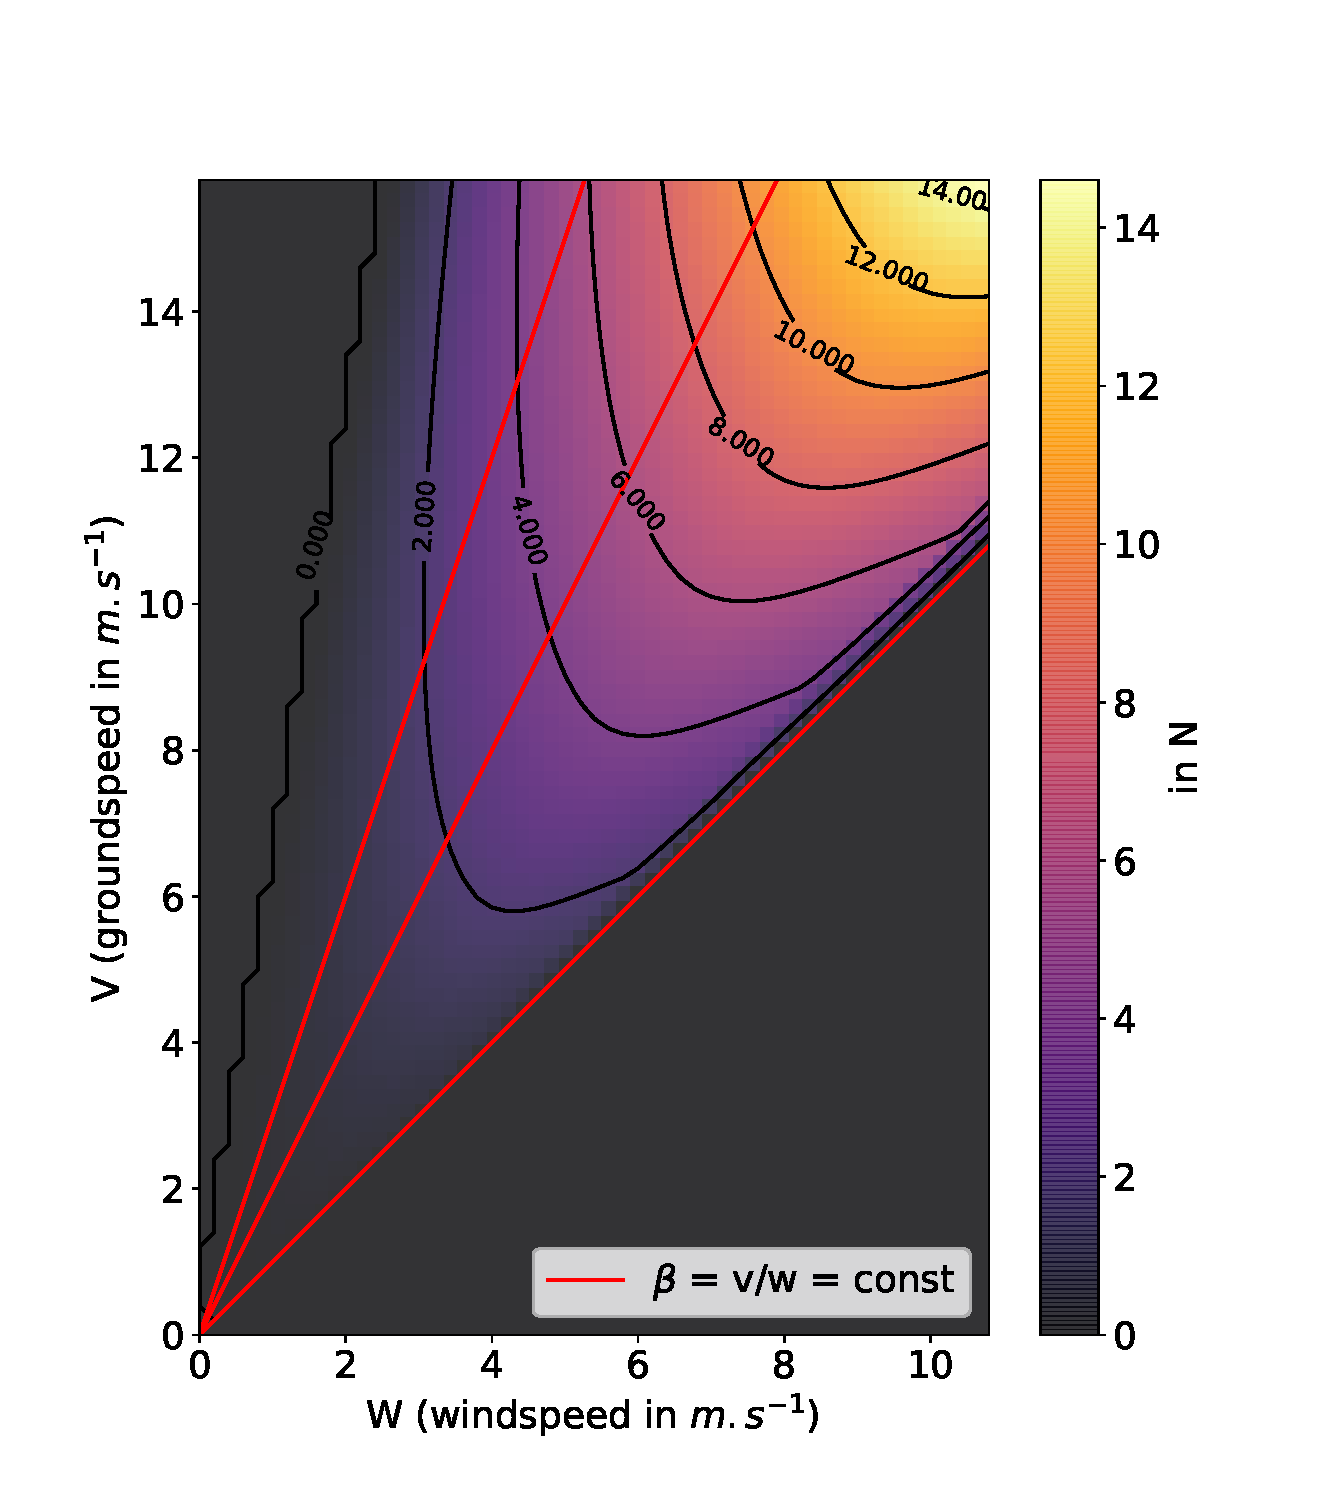
\includegraphics[width = 0.22\textwidth]{images/part6/naca6412-8a-78-10-5-3-470-6.pdf}
    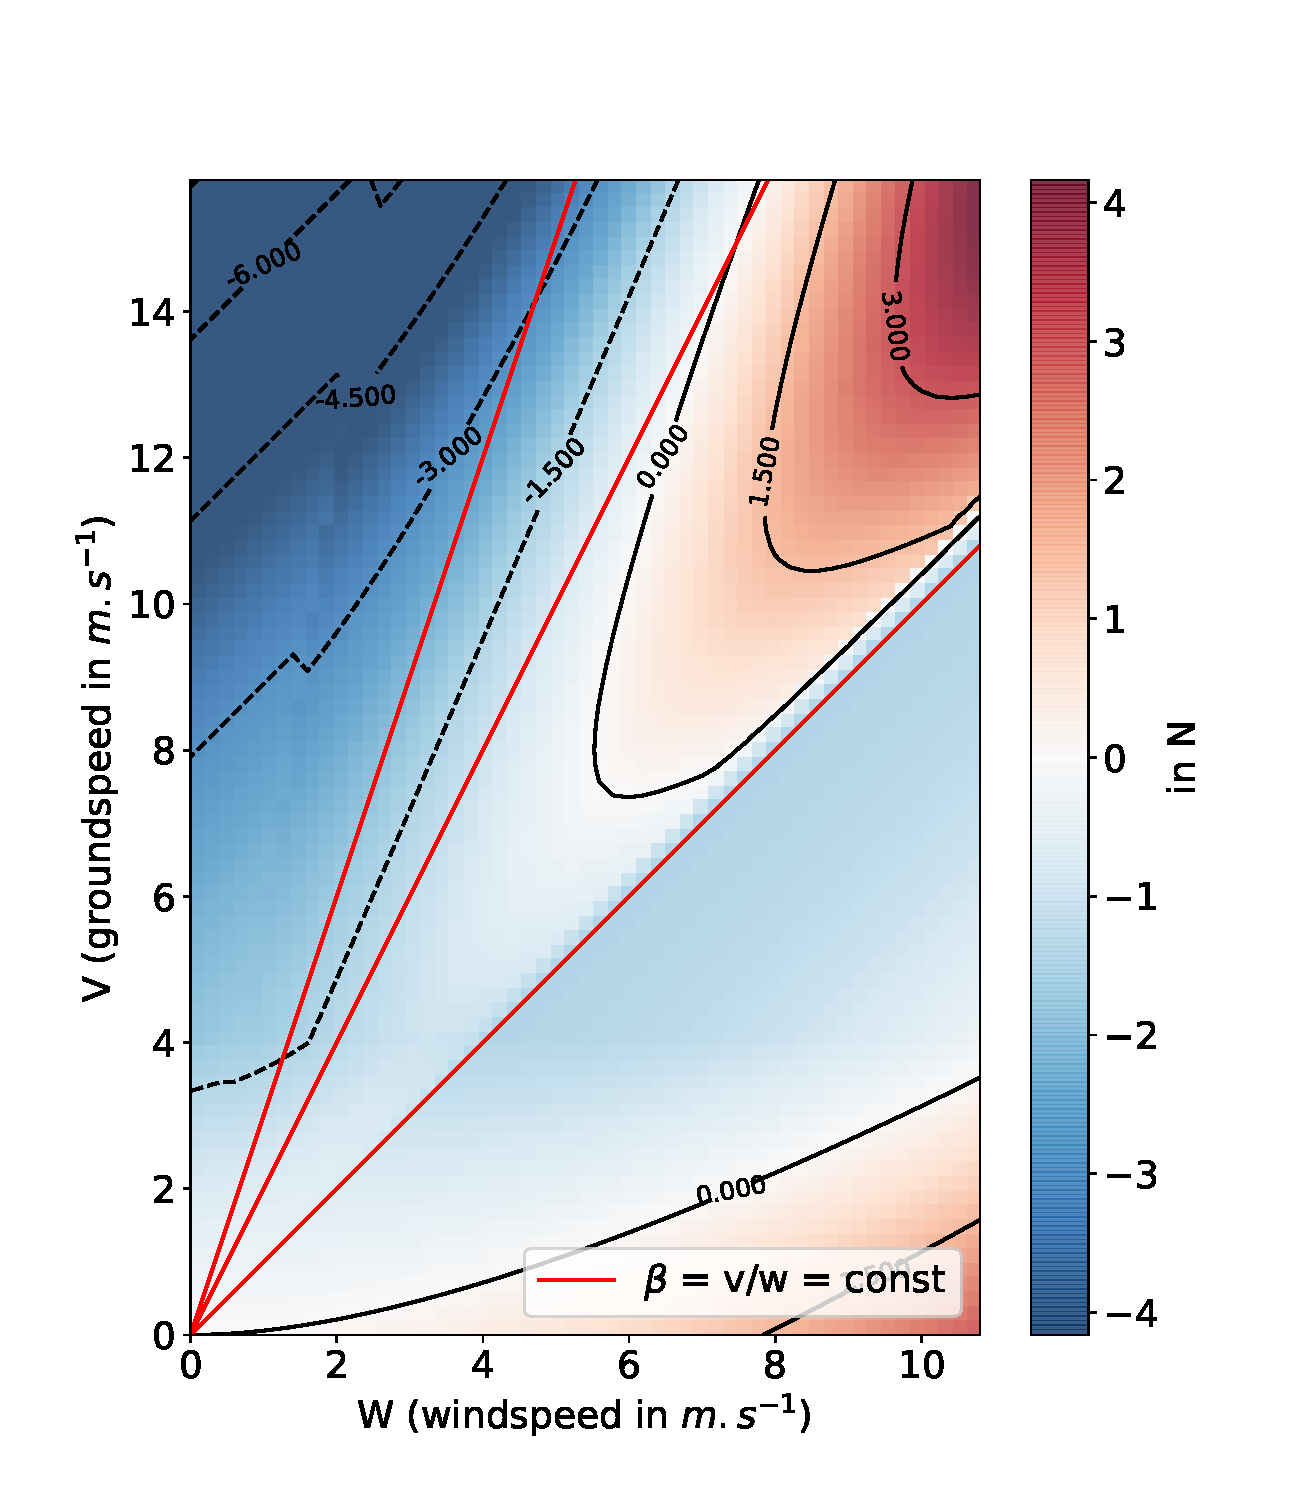
\includegraphics[width = 0.22\textwidth]{images/part6/naca6412-8a-78-10-5-3-470-6__total.pdf}
    
    \caption{Total force (left) and thrust (right) as a function of groundspeed and windspeed. Lines of constant speed ratio shown in red (with $\beta$ = 1, 2 and 3)}

    \label{fig:pythonresults}
\end{figure}

Iterating over various possible inputs then enabled us to converge to a more adequate propeller. From the model, it was found that a higher operating RPM would increase the overall efficiency of the propeller due to the higher operating Reynolds number. The chosen gear ratio to set the RPM operating range resulted from a compromise between propeller efficiency and safety of operations. It was found that using a gear ratio of 1 yielded an operating Reynolds number of about $1\times10^5$ at the mid-span, which was on the lower limit of what was deemed acceptable. This meant that for $40.6 \mathrm{cm}$ wheels and operating at $10 \mathrm{m/s}$, the RPM of the propeller was 463. 

The number of blades was also assessed. Given the diameter limitation of 80cm, the blade count had to be chosen to allow the propeller to generate enough thrust at the specified RPM (defined from manufacturing requirements later). Increasing the number of blades also meant a greater impact on the budget. From the model output, it was determined that a minimum of three blades would output the required amount of thrust while maintaining an efficient blade geometry as shown in Figure \ref{fig:jprop}.

\begin{figure}[!htbp]
    \centering
    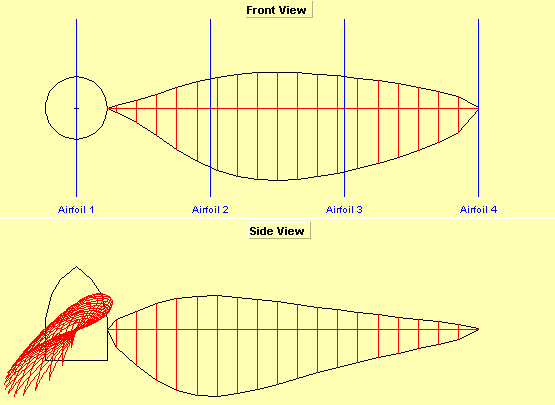
\includegraphics[width= 0.45\linewidth]{images/part6/javaprop2blades.png}
    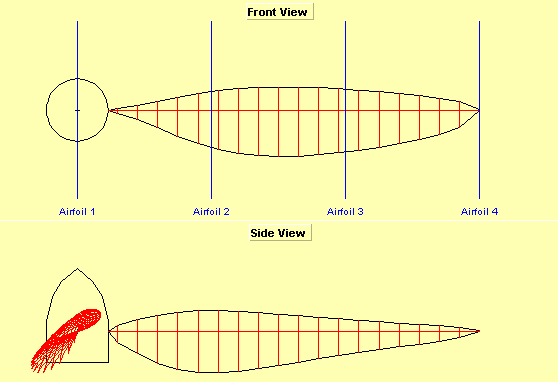
\includegraphics[width= 0.48\linewidth]{images/part6/javaprop3blades.png}
    \caption{JavaProp output geometry for a 2-bladed propeller (left) and a 3-bladed propeller (right) designed for equal thrust output}
    \label{fig:jprop}
\end{figure}

Several blade profiles were tested to assess their impact on the performance of the vehicle. The lift-to-drag ratios of the profiles were compared, as shown on Figure \ref{fig:clcdalpha}. It is clear from this plot that the NACA 6412 had a significantly better performance than the other two. Further investigations were conducted using the theoretical model. The main observation was that a higher cambered aerofoil blade profile would have a broader range of pitch over which the thrust was high in comparison to low camber and symmetrical aerofoil blade profiles. This is illustrated on Figure \ref{fig:aeroprofiles}. The NACA 6412 profile was chosen due to its higher performance at the relevant Reynolds number range as shown on Figure \ref{fig:clcdalpha}.

\begin{figure}[!htbp]
    \centering
    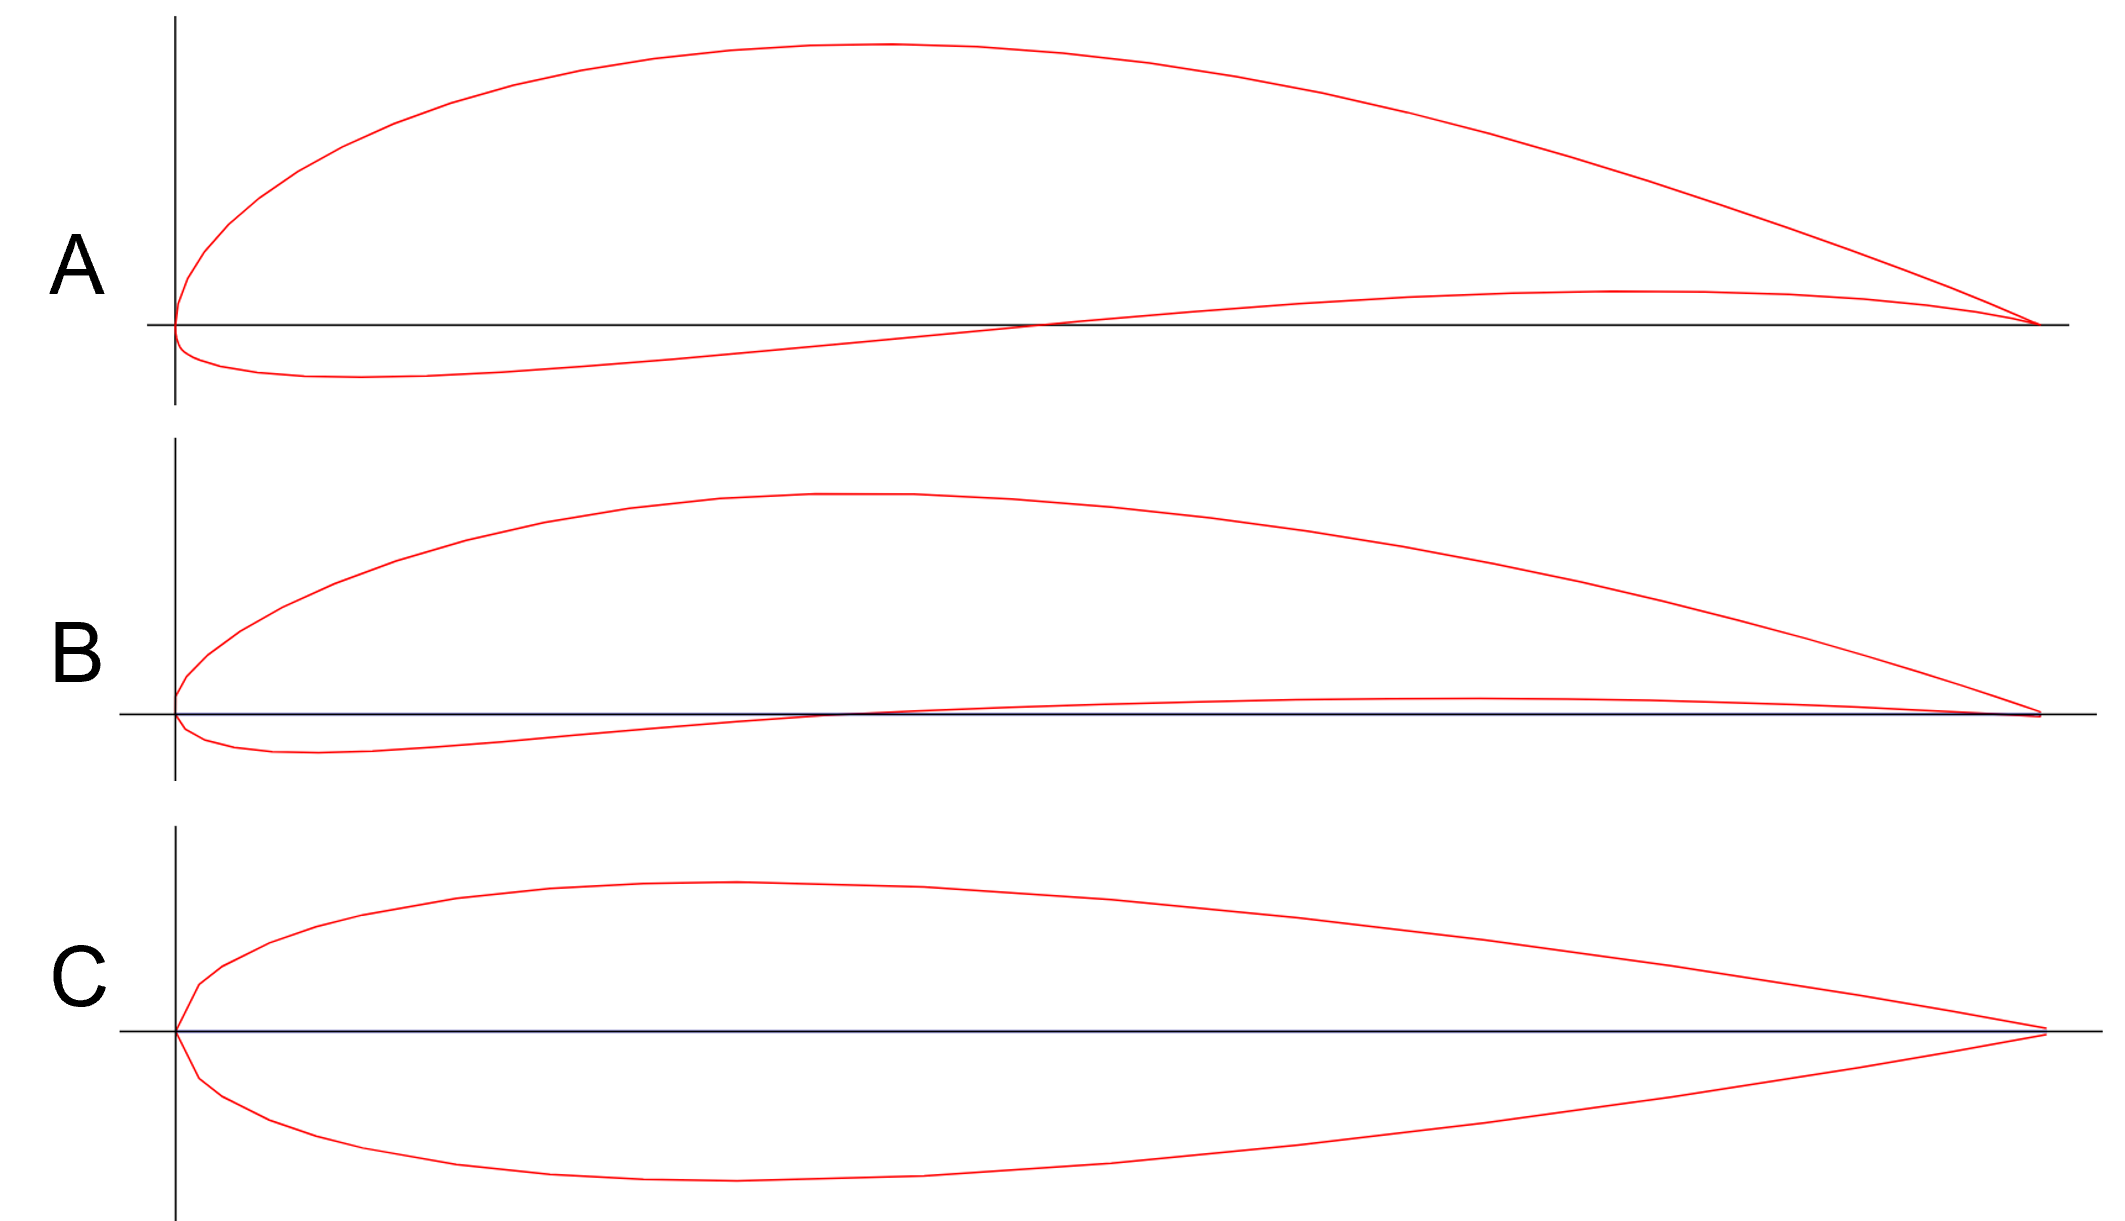
\includegraphics[width=0.4\linewidth]{images/part6/bladeprofiles.png}
    \label{fig:bladeprofiles}
    \caption{Assessed blade profiles: mh112 (A), NACA 6412 (B), NACA 0016 (C)}
\end{figure}

\begin{figure}[!htbp]
    \centering
    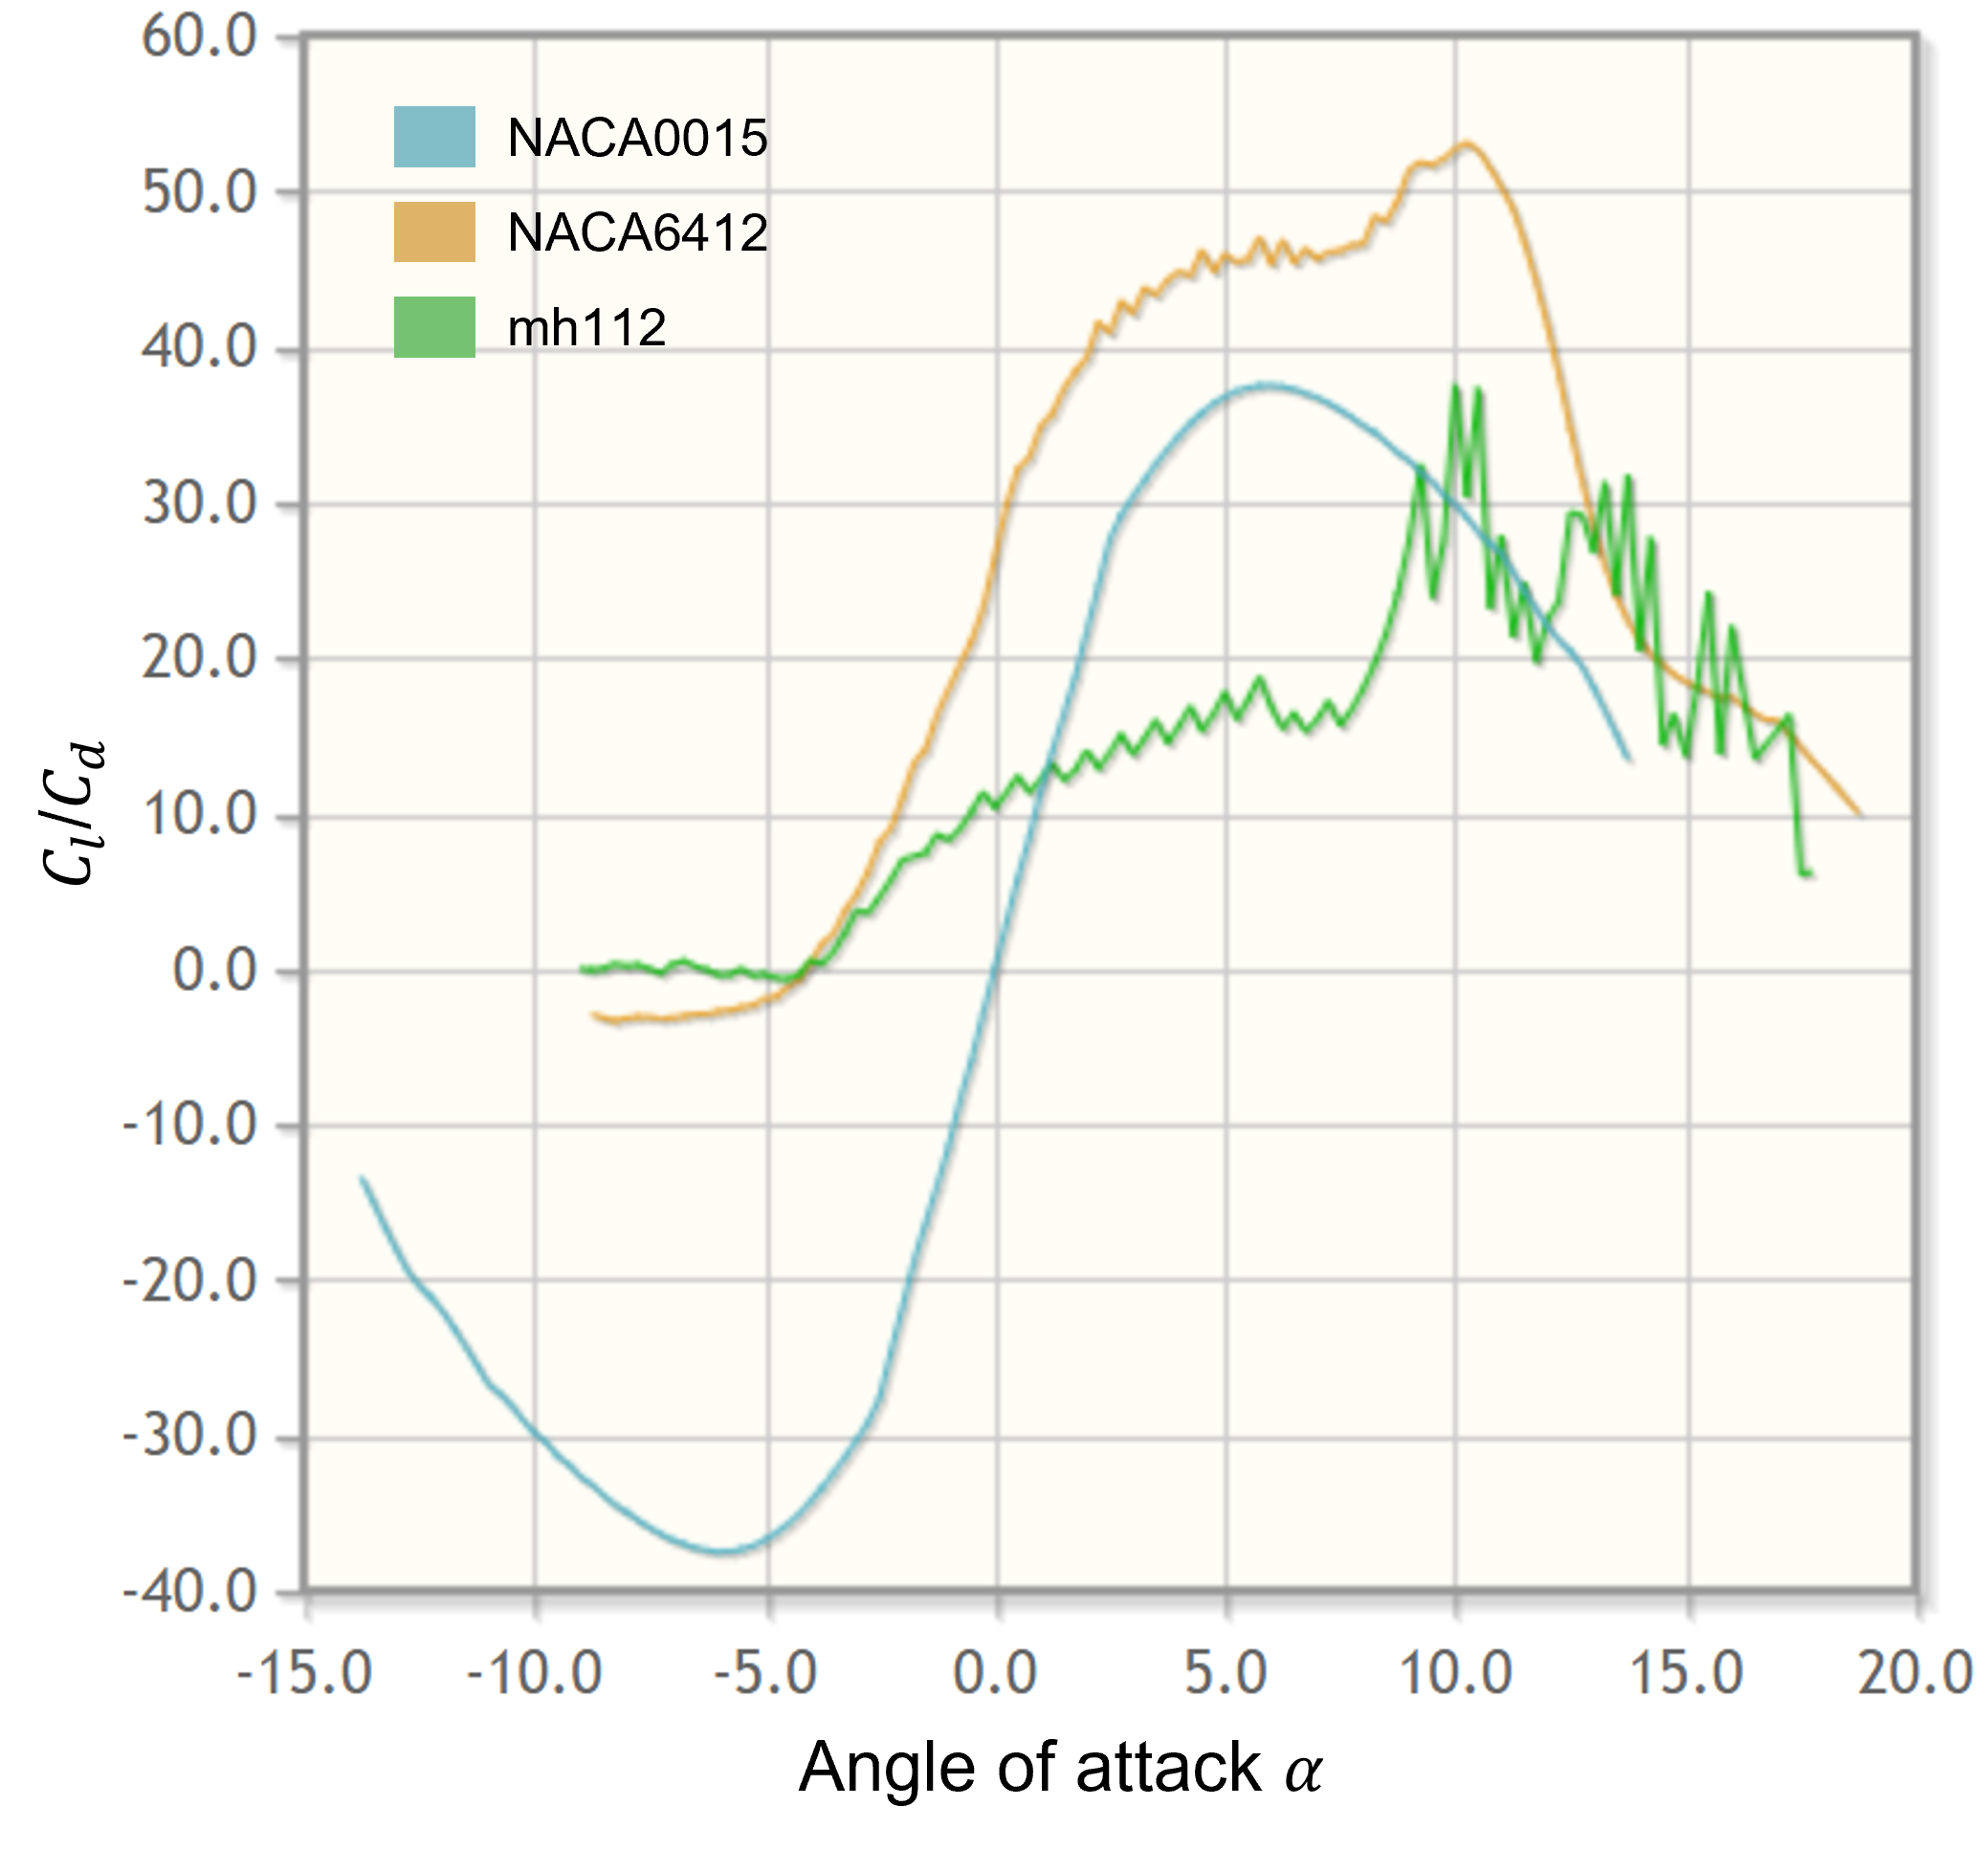
\includegraphics[width = 0.5\linewidth]{images/part6/clcdalpha.png}
    \caption{$C_l/C_d$ as a function of $\alpha$ for different blade profiles ($\mathbf{Re} = 1\times10^{05}$)}
    \label{fig:clcdalpha}
\end{figure}

\begin{figure}[!htbp]
    \centering
    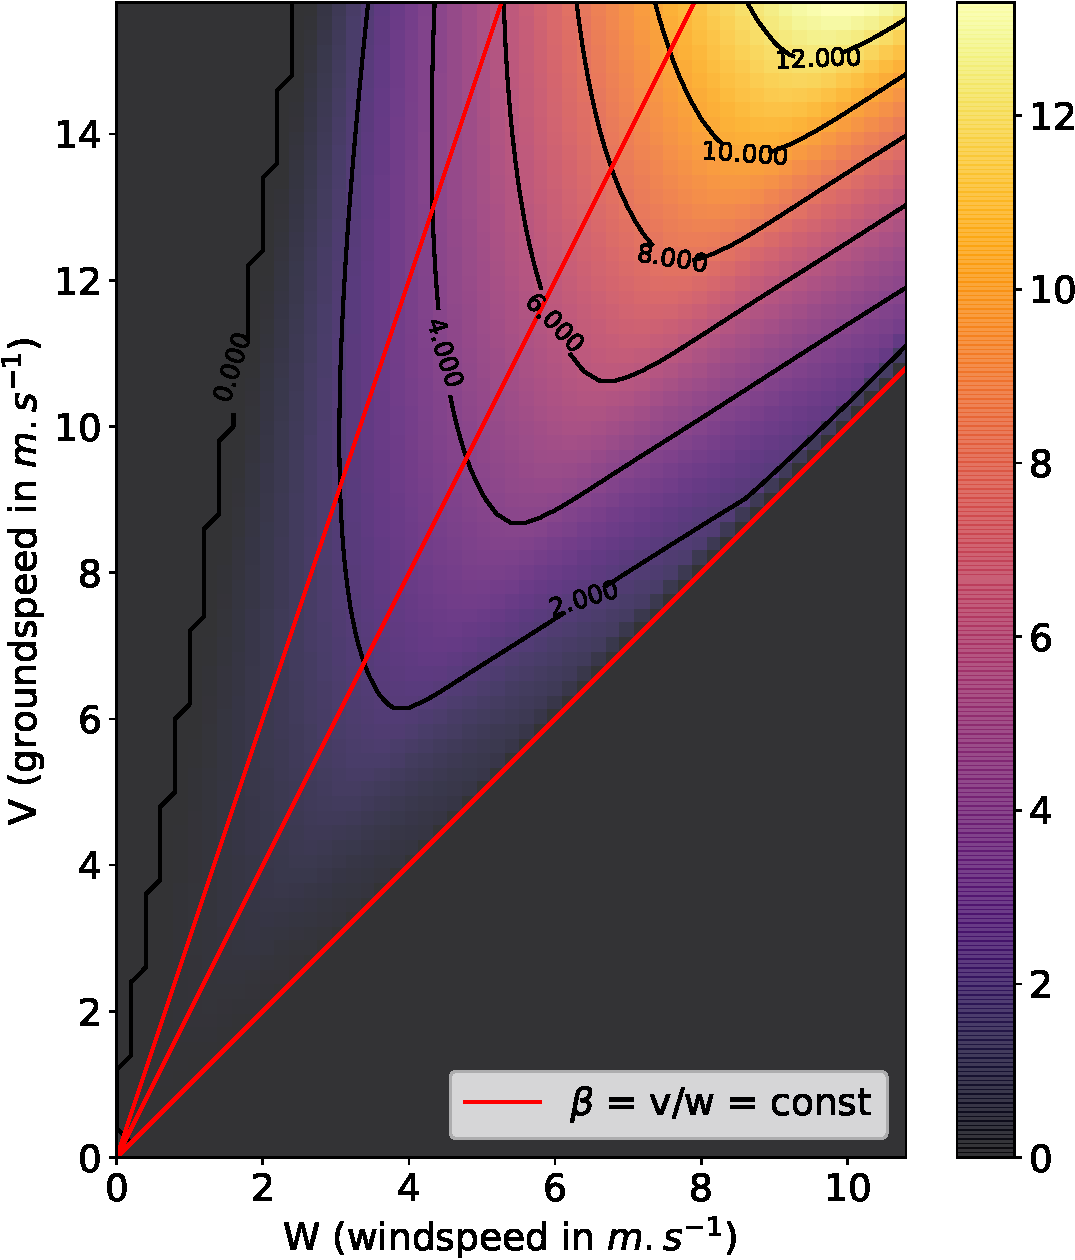
\includegraphics[width =0.1465\textwidth]{images/part6/naca0016.pdf}
    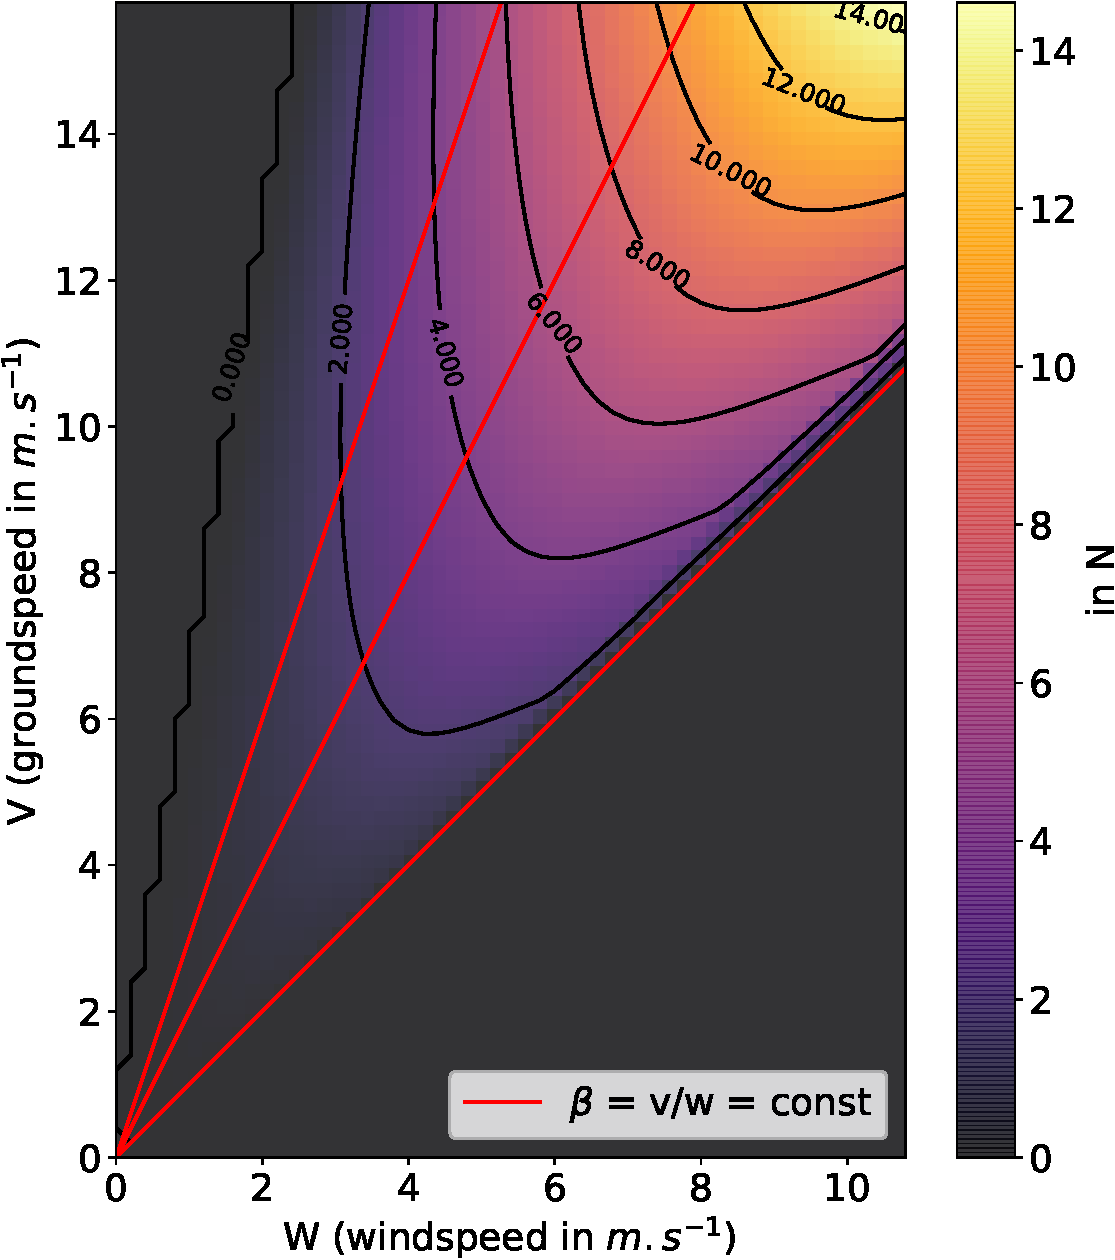
\includegraphics[width =0.152\textwidth]{images/part6/naca6412.pdf}
    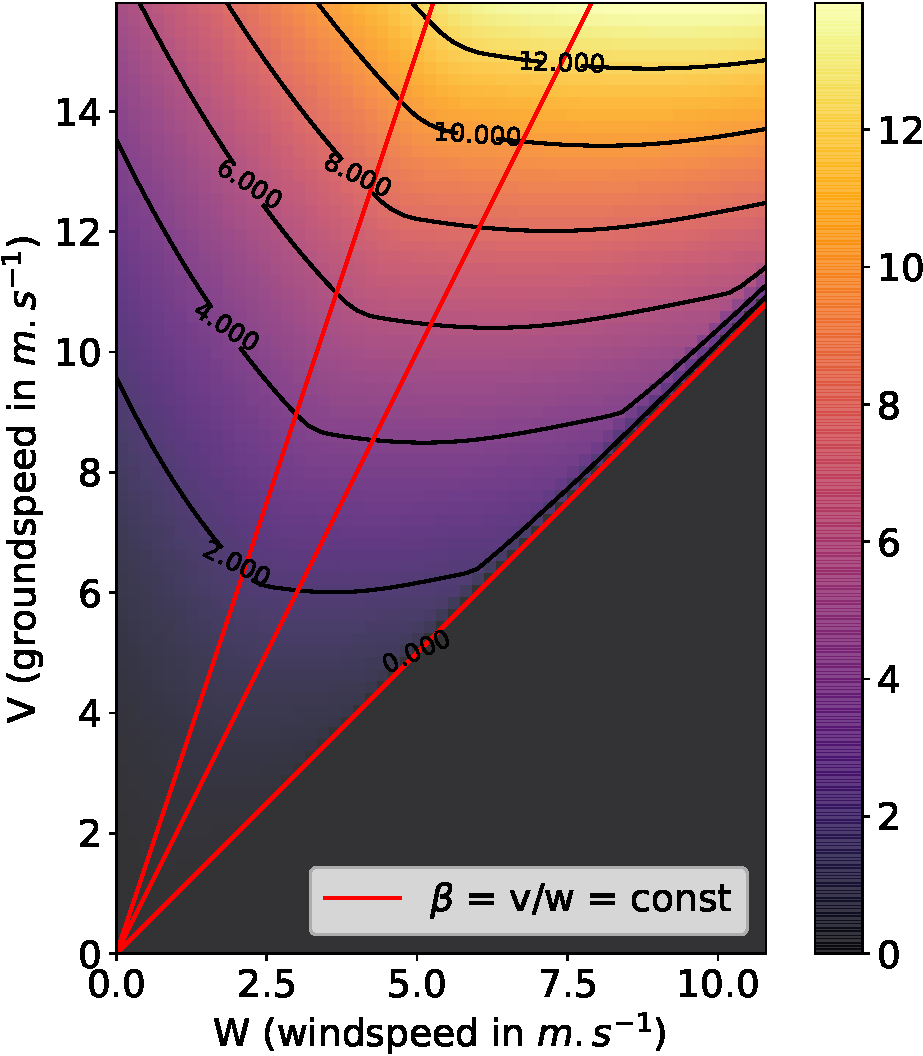
\includegraphics[width =0.15\textwidth]{images/part6/mh112.pdf}
    \caption{Propeller thrust as a function of groundspeed and windspeed. From left to right: NACA 0016, NACA 6412, mh112}

    \label{fig:aeroprofiles}
\end{figure}

It was then possible to converge towards a more efficient propeller design. Due to budgeting, and the limited impact of blade number on efficiency as stated before, the blade number was set to 3.

\subsection{Manufacturing}

The manufacturing process of the propeller had a high impact on the design choices. It was initially decided that the best course of action would be to buy an off-the-shelf propeller and in parallel, further improve a custom geometry and manufacture it further down the line. After surveying the market for off-the-shelf propellers in the size range required, it was made clear that there were not any suitable options for application in this project. The available rotors being designed for model aircraft and other similar applications did not feature an adequate pitch nor the possibility of modulating it. This meant that modifications would have to be made to the blades. Being made for high RPM applications (2000+ RPM) and a lower pitch than desired, restructuring the blades and using them on a custom hub would lead to safety concerns. Also, the lower efficiency provided by propellers featuring a low number of blades (2 in this case) was a non-negligible drawback in this case, where efficiency is key. Consequently, as the price for off-the-shelf propellers was quite high, and the predicted performance quite low, more focus and effort was put on designing and manufacturing the custom propeller.

Several possibilities were outlined when it came to manufacturing the propeller, of which were carbon fibre layup, aluminium machining, metal printing, and PLA 3D printing. Each one of these materials had mechanical properties suitable for high-RPM operations as determined by modelling the blades as rectangular and finding the tensile strength of the root which is highly stressed under centrifugal loading (Table \ref{fig:mattable}).

\begin{table}[!htbp]
    \centering
    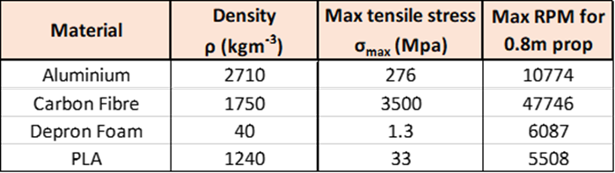
\includegraphics{images/part6/materialstable.png}
    \caption{Material strength analysis for propeller}
    \label{fig:mattable}
\end{table}

Due to the lack of experience in the team required to perform carbon fibre manufacturing and high associated costs, this option was ruled out. A mix of aluminium and PLA 3D printing was chosen as this would exploit the strength of aluminium for load bearing components, and the low cost, easy changeability of PLA parts for the most aerodynamic sections of the blade.

The mid-section of the propeller would be 3D printed in PLA in two parts (Due to the vertical orientation of parts to align the layer lines with the flow direction) whilst the tips and roots of the blades would be 3D printed in aluminium and held together by a rod running through all sections. This meant that the centrifugal load on the PLA sections would be transferred to the aluminium tip, connected to the root by the spar. Doing this ensures the 3D prints experience only compressive loads and cannot delaminate. This combination limits the costs and weight of the blades, with a roughly 68\% mass saving over an entirely aluminium equivalent. An additional benefit was the possibility to reassemble the blades with various midsections to generate improved geometries from testing, whilst retaining the aluminium root and tips. These geometries could then easily be replaced and fitted on the blade rods. An exploded view of this design is shown in Figure \ref{fig:propExploded} and explained in further detail later.

Propeller blades experience maximum stress at their root due to the centripetal force produced by the mass above them. Using a simple rectangular blade model, the minimum diameter of an aluminium spar required to carry the centripetal load at 2000 RPM (significantly higher than operational speeds) and a safety factor of 2  would be 2.1 mm. The decision was therefore made to use a 4 mm diameter spar as this would suitably handle the expected loads whilst comfortably fitting within the thickness of the blade. Integrating a thread into one end for securing nuts would yield a thread stripping shear strength in excess of 350 kg (3.48 kN), whilst the propeller would see loads up to 60 kg (580 N) at 2000 RPM. This result is typical of the safety margins of the propeller design, and even with the imperfect manufacture of components, the likelihood of failure is incredibly low.

An initial design of the custom propeller was achieved before Christmas as shown in Figure \ref{fig:propExploded}. In total, 8 different parts were designed. Some of these were to be manufactured by EDMC (4, 5, and 7). The PLA 3D-printed parts were to be manufactured directly by the team (1-3). Due to technical issues with the metal 3D printer, the initially designed roots and tips (4 and 5) had to be replaced with suitable alternatives, so the roots were then also 3D printed in PLA (4*), while the tips were replaced with water-jet cut aluminium sheets (5*). The new tip replacement parts were then welded to the spar, as initially planned, such that the load experienced by the tips was transferred to the spar. These changes are shown in Figure \ref{fig:propExploded} by the initial and revised design following these manufacturing complications, with parts outlined in Table \ref{tab:propParts}.

\begin{figure}[!htbp]
    \centering
    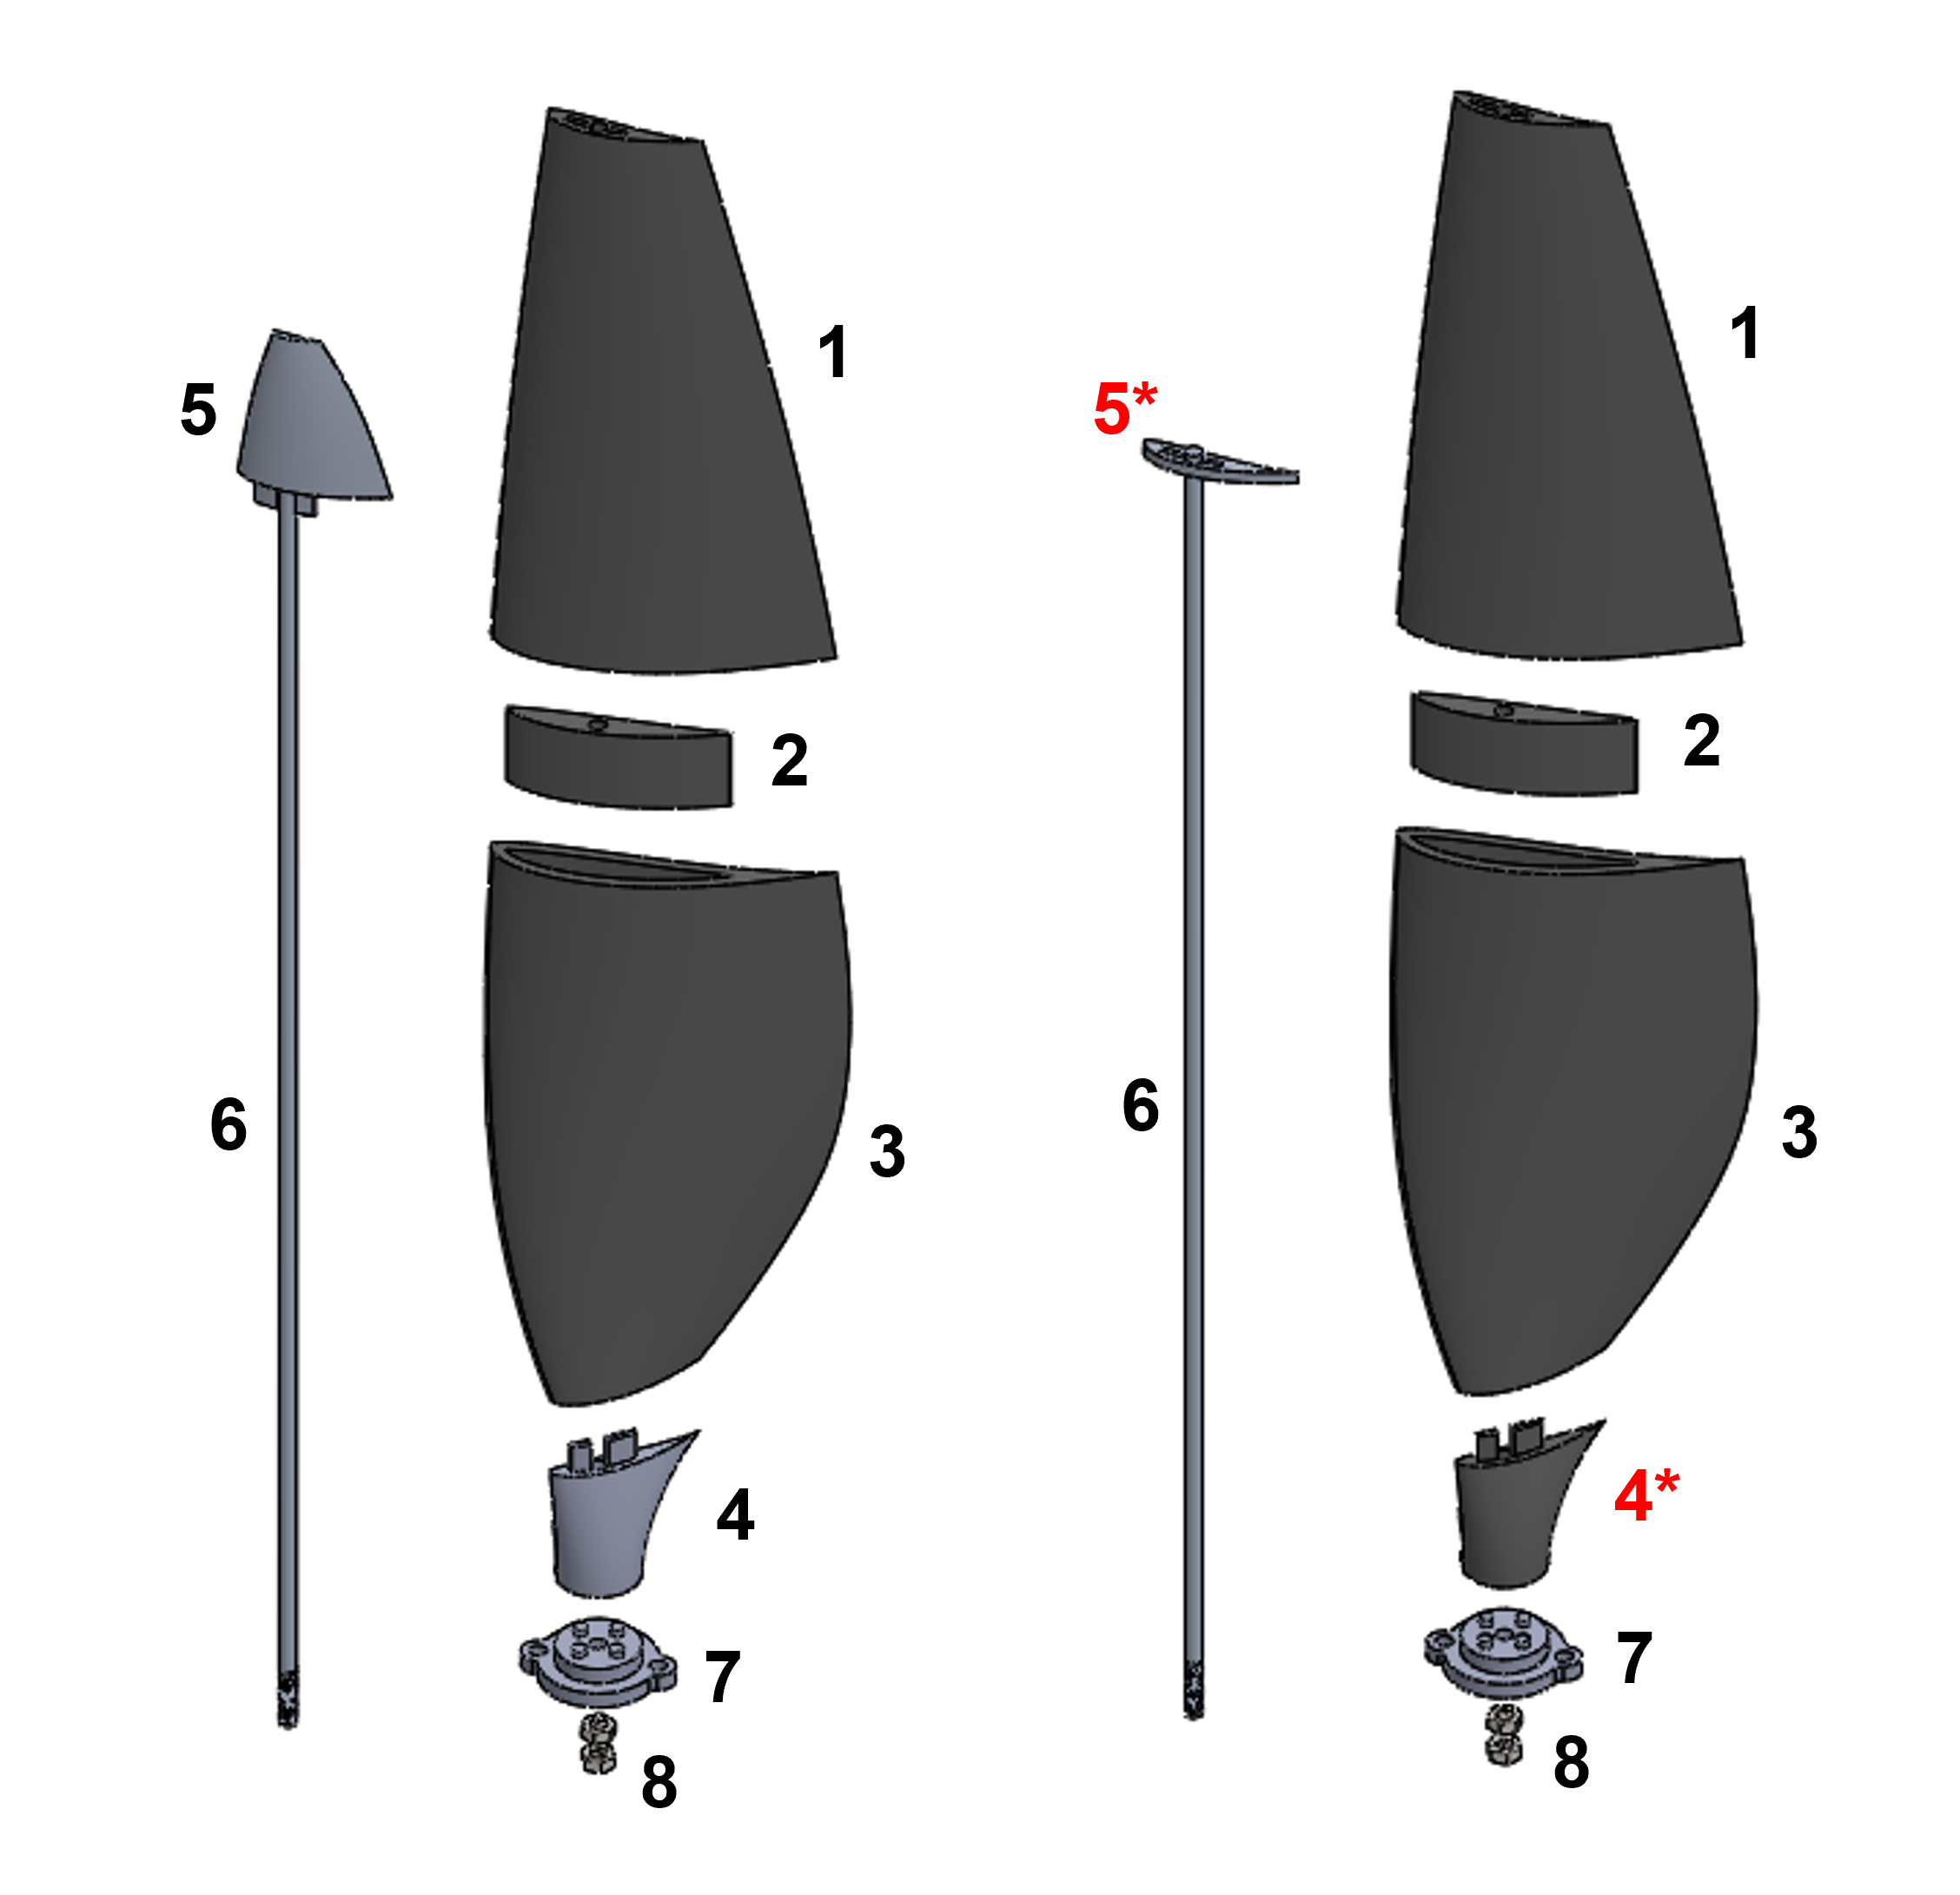
\includegraphics[width=0.7\linewidth]{images/part6/propExploded.png}
    \caption{Exploded view of final propeller design (left) and revised design (right)}
\label{fig:propExploded}
\end{figure}

\begin{table}[h]
\centering
\begin{tabular}{cllc}
\rowcolor[HTML]{C0C0C0} 
\multicolumn{1}{l}{\cellcolor[HTML]{C0C0C0}\textbf{Part No.}} & \textbf{Description}         & \textbf{Material} & \multicolumn{1}{l}{\cellcolor[HTML]{C0C0C0}\textbf{Quantity}} \\
1                                                             & 3D printed upper section     & PLA               & 1                                                             \\
2                                                             & 3D printed alignment coupler & PLA               & 1                                                             \\
3                                                             & 3D printed lower section     & PLA               & 1                                                             \\
4                                                             & Metal 3D printed root        & Aluminium         & 1                                                             \\
4*                                                            & 3D printed root              & PLA               & 1                                                             \\
5                                                             & Metal 3D printed tip         & Aluminium         & 1                                                             \\
5*                                                            & Water-jet cut tip            & Aluminium         & 1                                                             \\
6                                                             & Ø4mm propeller spar          & Aluminium         & 1                                                             \\
7                                                             & CNC machined root mount      & Aluminium         & 1                                                             \\
8                                                             & Securing nuts                & Stainless Steel   & 2                                                            
\end{tabular}
\caption{Propeller blade table of parts}
\label{tab:propParts}
\end{table}

After much 3d print testing to ensure suitable mass, strength, tolerances, and surface finish, two sets of final blades were produced with a layer height of 0.1 mm and infill of 20\%. The surface was then smoothed with 140 to 3000 grit sandpaper to remove all traces of layer lines that could interfere with the flow and finished with brass polish. Due to minor unavoidable warping with the prints, small gaps existed between the assembled parts, so were filled with excess PLA scraps and glued together. Each blade was then fully assembled with the additional aluminium components and nuts secured with thread locking adhesive to prevent vibration loosening during tests. Figure \ref{fig:bladeComplete} displays the completed blade ready for insertion in the hub.

\begin{figure}[!htbp]
    \centering
    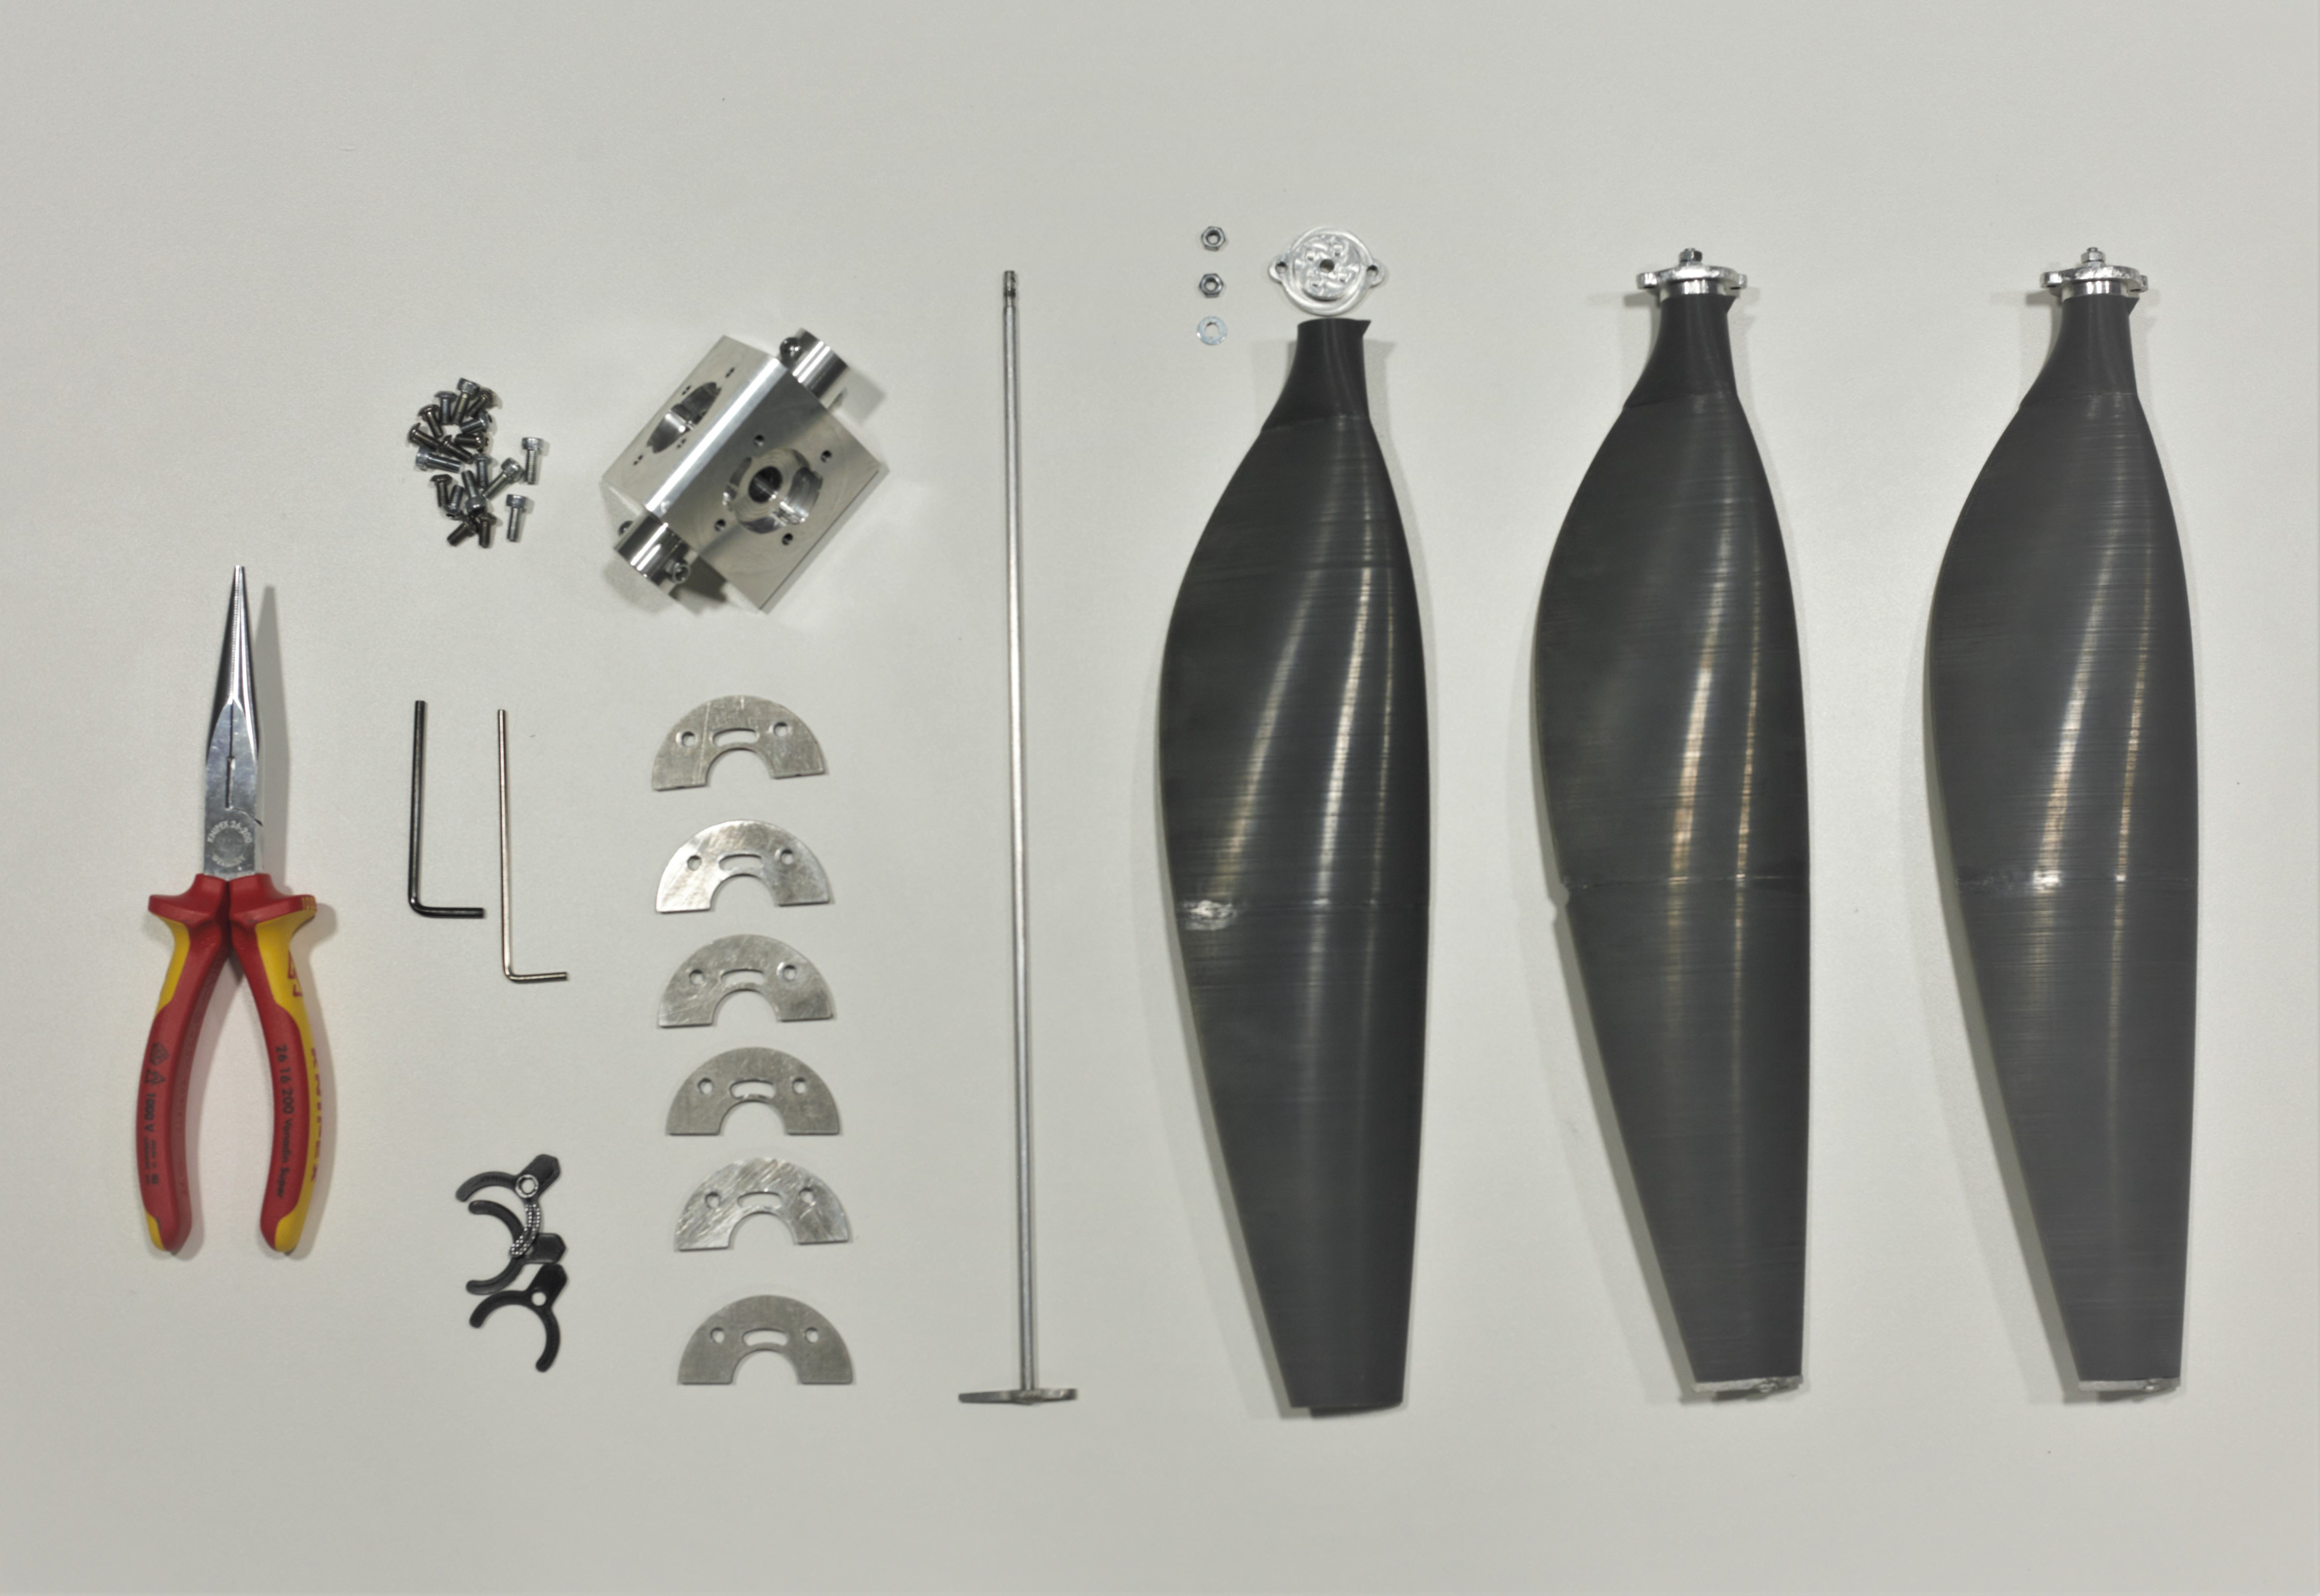
\includegraphics[width=0.7\linewidth, angle=180]{images/part6/buggabugga.jpg}
    \caption{Final manufactured propeller disassembled and all the tools required to assemble it.}
\label{fig:bladeComplete}
\end{figure}



%\cleardoublepage
\section{Final Design Proposal}
\subsection{Structure}

\begin{figure}[H]
    \centering
    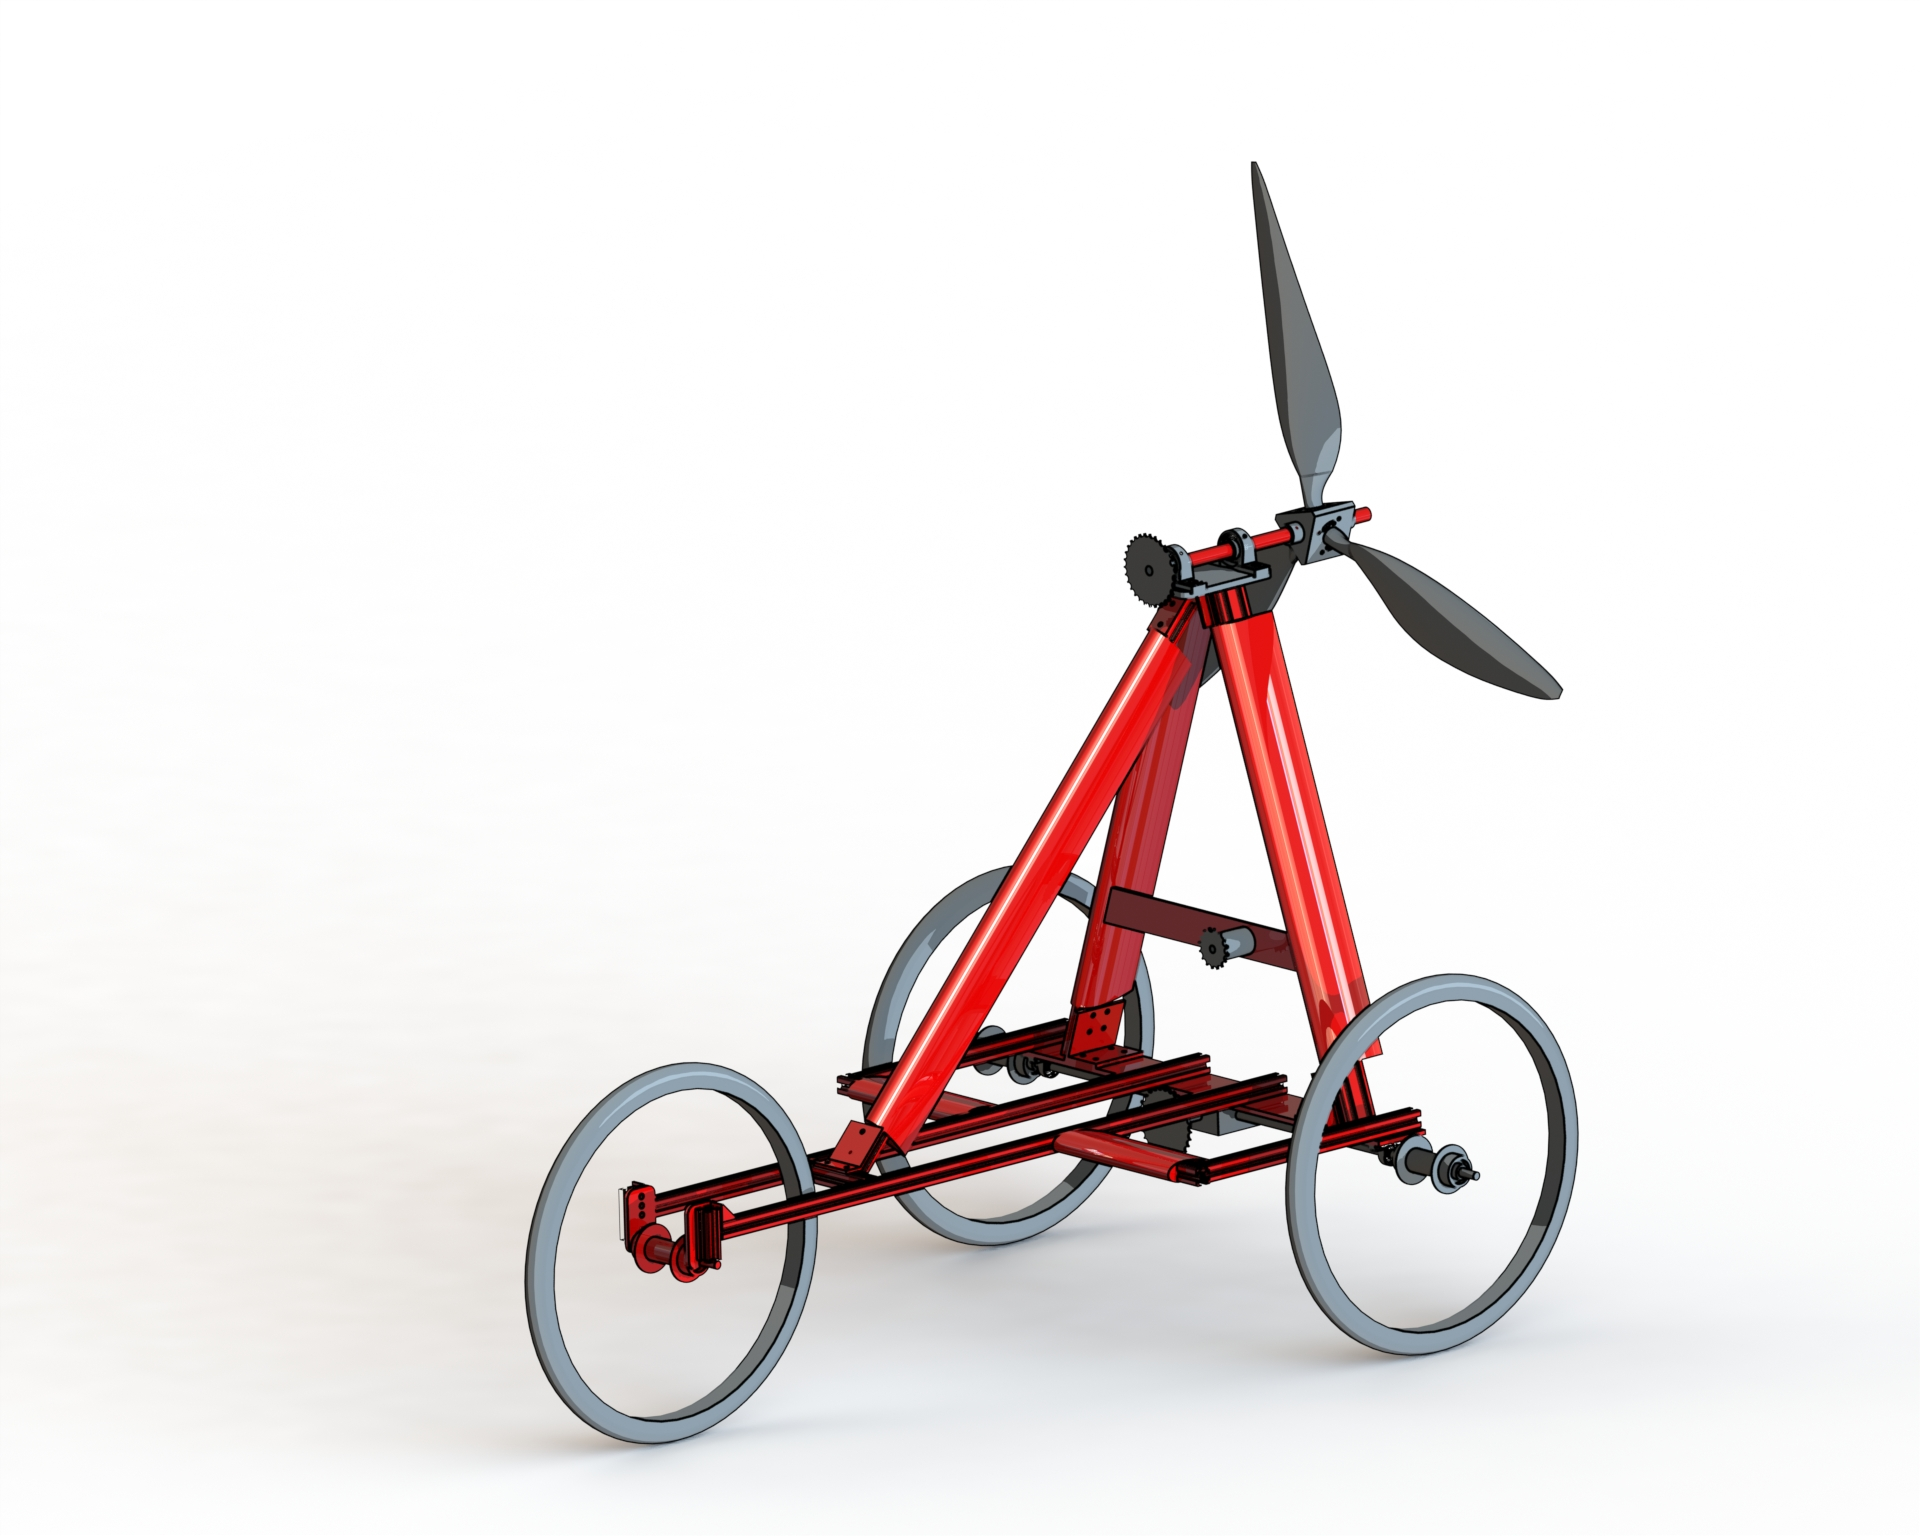
\includegraphics[width = 0.5\linewidth]{images/renders/structure.JPG}
    \caption{Structure of the prototype}
    \label{fig:structrender}
\end{figure}

The overall structure is a construction weighing 11kg, excluding the propeller (Figure \ref{fig:structrender}). It is comprised of mainly aluminium profile 20x20 mm and 20x40 mm beams, aluminium plates, all bolted together and connected to the drivetrain, propeller shaft, and wheels. The structure is a simple, stiff design which effectively facilitates testing in the wind tunnel as per the project requirements. The vehicle length is 1137 mm, the height including the top sprocket (propeller dismounted) is 820 mm, and the maximum width at the rear is 800 mm. The vehicle is lightweight due to the use of aluminium parts and by efficient use of material.


\subsection{Drivetrain and transmission}

\begin{figure}[H]
    \centering
    \includegraphics[width = 0.5\linewidth]{images/renders/drivetrain.JPG}
    \caption{Transmission of the prototype}
    \label{fig:transmirender}
\end{figure}

The final transmission system  (Figure \ref{fig:transmirender}) consists of an axle shaft connected to a chain through a right-angle gearbox. This chain drives the propeller shaft situated on top of the vehicle. The chain is kept in tension by a chain tensioner mechanism which can be adjusted based on the needs. The gear ratio between the prop-shaft sprocket and driven sprocket is 1:1, both 30 tooth, with an 8mm pitch chain running between them. The chain tensioner sprocket used is 24 tooth, running on a bearing to minimize resistance and mounted to an aluminium plate fixed to the A-frame.

\subsection{Propeller and hub}

\begin{figure}[H]
    \centering
    \includegraphics[width = 0.5\linewidth]{images/renders/prop.JPG}
    \caption{Propeller and hub of the prototype}
    \label{fig:proprender}
\end{figure}


The final propeller (Figure \ref{fig:proprender}) is composed of 3 blades featuring the ability to vary the pitch angle by $20^\circ$ in both directions. It is 780 mm in diameter. The blades used a NACA 6412 profile along the entire PLA 3D printed mid-section. The blades can be swapped out for different ones within minutes with the highly modular design. This also implies that transportation of the propeller is facilitated. The hub has a diameter of 71 mm and is designed to fit on a 16 mm shaft.



\section{Experimental Testing and CFD Methodology}
One of the aims of the project was to test the vehicle in a controlled environment to acquire data and assess the vehicle’s performance. This would allow for further developments on the vehicle but also further the understanding of the concept and what it takes to build a downwind faster than the wind vehicle. With the prototype being too large to be tested on a treadmill as had been done previously by Rick Cavallaro in \cite{rick2008youtube}, the best option for testing the vehicle in a quantifiable way was to use the rolling road in the R.J. Mitchell Wind tunnel at the University of Southampton. Before testing, the main quantities for which data was to be acquired were outlined. Included, were the drivetrain efficiency, vehicle drag and overall performance. The completed tests ran the vehicle on the rolling road in the wind tunnel with wheel arm mounts holding the vehicle in place. Aerodynamic drag values for the vehicle were obtained in both directions.

\subsection{Inputs} 

For the wind tunnel test, there were four main inputs for each experimental test: the rolling road speed, wind speed, propeller blade pitch and the gear ratio. It was initially intended to have an interchangeable gear ratio. However, the sprockets were made from hardened steel, so the gear ratio had to be fixed because threading these components was not feasible with the available means. A 1:1 chain gear ratio was chosen as this outputted the right RPM for the propeller given the wheel size. The chain sprockets were then welded to the gearbox shaft. The rolling road speed was varied for each test case, starting at low speeds and increasing in increments of $0.5\mathbf{m/s}$ or $1\mathbf{m/s}$ to ensure that a wide range of testing cases were available for analysis. Modulating the pitch of the propeller would help in finding an optimal setup to maximise performance, hence furthering the understanding of the characteristics of the DWFTTW prototype. The vehicle was monitored at all points during testing to ensure normal operation and avoid catastrophic failures.

\begin{figure}[!htbp]
    \centering
    \includegraphics{images/part10/chaincog.jpg}
    \caption{Sprocket welded to propeller shaft}
    \label{fig:weldedsprocket}
\end{figure}

\subsection{Wind tunnel testing plan}

A test session of three consecutive days was initially intended in the R.J. Mitchell wind tunnel. This would ensure the completion of all the planned tests while sparing the time required for setting experiments up. From analysis, three main test conditions, to simulate a normal vehicle operational environment, were outlined. The cases are looking at the vehicle under slower than, the same speed as, and faster than the wind regime.

\begin{figure}[!htbp]
    \centering
    \includegraphics[width=0.4\linewidth]{images/part10/expebaseline.jpg}
    \includegraphics[width=0.4\linewidth]{images/part10/fasterthanwind.jpg}
    \caption{"Baseline" experimental setup (left) and "faster than wind" experimental setup (right).}
    \label{fig:baseline}
\end{figure}

With the aim being to determine the maximum speed the vehicle was able to reach, several experimental setups were defined. The case in which the ground speed is equal to the wind speed was the simplest scenario to recreate as is illustrated in the baseline diagram in Figure \ref{fig:baseline} (left). It required the rolling road to be moving along with the vehicle mounted on top. This test was run to determine which drag or thrust was produced while the vehicle was moving at wind speed. Based on the outcome, various testing setups were defined to simulate the relevant operating conditions. This setup will be referred to as the baseline setup for added clarity. For faster than the wind operation Figure \ref{fig:baseline} (right), the wind tunnel was to be used in combination with the rolling road to simulate on-coming wind.

Due to the rolling road only being capable of operating in the same direction as the wind flow, reproducing slower than wind operation was less direct. To achieve it, one of the considered options was to rotate the vehicle in the wind tunnel test section while inverting the gearbox to run the drivetrain in reverse. This made it possible for the prototype to run with the wind differential pushing it, yielding insight into how this would affect performance. However, this option was not carried out as it would have meant additional precious time being spent setting up. It also introduced the requirement to reconfigure to the gearbox, which was meant to be welded. The other option for this case was to run the baseline setup and quantify the rolling resistance. In turn, from this and the before-hand quantified drag, the equilibrium point could be determined analytically by summing the various forces.

\subsection{Project timings}

The initial wind tunnel testing plan was a three-day testing period in which all the measurements and analysis would be completed as well as some further testing for the visual experiments. Time management proved crucial for this project as planning the wind tunnel days had to be done well in advance. Therefore, early contact was made with the wind tunnel team, so that the tests could be designed and organised as early as possible. Regular meetings were arranged to facilitate progress and impose strict deadlines for manufacturing and design.

Despite this, due to manufacturing issues, the propeller was not ready before the planned three-day testing period. Some experiments could be carried out by disregarding the propeller, but complete vehicle testing was not possible. Hence the test sessions were split into two sets: a one day session to test the drivetrain, then a two days session to test the full vehicle operation. This meant that a first test could be carried out without the propeller, but also conveniently sparing time for the EDMC to finish the missing parts. It also became possible to spot potential issues with the structure of the vehicle early thanks to the first test and have enough time before the next wind tunnel session to correct them. The first test day was conducted in mid-February while the second was completed in March.
 

\subsection{Load measurement using the rolling road}

The best way of quantifying the loss contribution of each element of the vehicle was to use the wind tunnel’s rolling road and measure the increased drag force on the system induced when adding each component to the vehicle. By running the rolling road at a set range of velocities, measurements of the force applied to the vehicle could be taken using the load cells mounted on each side. The force required to overcome each element of the vehicle added gradually was plotted, and the losses induced by each component was quantified.

The data collected for this experiment was comprehensive and covered all the main drivetrain components meaning an in-depth analysis of the limiting factors of the vehicle could be completed. Although this experiment quantified the loss contributions of many components of the prototype, no way could be found, given the available installations, to evaluate the efficiency of the propeller shaft bearings. Therefore it was not possible to dissociate the contributions of the chain and the top bearings to the losses without speculating or making further assumptions that were out of the scope of this project.


\subsection{Load cell and force measurements}

The load cell was the main point of connection for the vehicle to the mounts of the wind tunnel. The decision on what load cell mounts to use and how to use them was important during the thinking of the wind tunnel test. Two load cell mounting options were considered in this case: the overhead balance and/or the wheel arms. Both mounts required external structural extensions on the vehicle, which needed to be taken into consideration.

\begin{figure}[!htbp]
    \centering
    \includegraphics{images/part10/wheelmounts.png}
    \caption{Wheel arm mounts experimental setup}
    \label{fig:wheelmounts}
\end{figure}

The wheel mount connections available in the wind tunnel allow the load cells to be attached to the side of the vehicle. This method offers a single degree of measurement for the test, measuring the drag/thrust of the vehicle. The stabilization of the load cells will provide enough restoring moment on the vehicle, meaning the vehicle will remain 
straight throughout the test. This increased the safety of the experiment and reduced the chances of causing damage to the vehicle or wind tunnel. With this method the force were measured on both sides of the vehicle, meaning the measurements were split. The voltage changes measured through the Wheatstone bridge circuits were therefore divided by two, introducing the need to have a high enough minimum resolution.


\begin{figure}[!htbp]
    \centering
    \includegraphics{images/part10/mountstruct.png}
    \caption{Structural extension possibilities. Option (1) on the left and option (2) on the right}
    \label{fig:mountstruct}
\end{figure}

\subsection{Two-wheel arm setup mounting}

Once the horizontal stabilisers were designed to be two straight bars going towards the front wheel, the focus turned to ensure that the model could be connected to the wheel arms of the wind tunnel. The issue faced was that there were no stable connections for the load cells to screw into. It was therefore required to design additional load cell connections for the wheel arms that would not affect the vehicle.

The closest part of the vehicle to the load cells would have been the axle rod of the back wheels. This component spins at the same RPM as the propeller and therefore would not be able to be directly connected to for a stable connection for the load cell. To overcome this issue, pillow bearings for the axle rod were used to allow components to be connected to the vehicle. 

The pillow bearings used allowed for the aluminium profile to be drilled and connected with screws which was beneficial for the vehicle as it maintained the modularity of the structure. To increase the stability of the load cell connection it was required to secure the bar to another section on the vehicle. This meant that the load cell would not oscillate significantly when the vehicle was rolling on the rolling road.

After consideration the two main locations for connecting the bar were the front wheel structural connections (1) and the metal plate on the other side of the wheel (2):


\begin{table}[H]
\caption{Advantages and disadvantages for the location of the wheel arm connection}
\label{tab:wheelArmConnection}
\centering
\begin{tabular}{|
>{\columncolor[HTML]{\CellColor}}l |p{7cm}|p{7cm}|}
\hline
\textbf{Option} & \cellcolor[HTML]{\CellColor}\textbf{Advantages}                                                           & \cellcolor[HTML]{\CellColor}\textbf{Disadvantages}                                                                   \\ \hline
\textbf{1}      & Stronger connection, less material used, added structural components to   the horizontal stabilisers. & Deformation with the vehicle oscillation possible, more pressure on   ensuring that the measurements are connect \\ \hline
\textbf{2}      & Mitigated deformation, as the bars are connected to two parts that are   mounted on the axle          & Increased material use, more cuts of the bar to manufacture                                                      \\ \hline
\end{tabular}
\end{table}

It was decided that it was better to connect the load cell mounts directly to the horizontal stabilisers of the vehicle to ensure that the structure would have the largest stiffness possible.

\subsection{Calibration}

Before the wind tunnel tests, an assessment of the load cell resolution was necessary to ensure force variations of the scale of those anticipated would be picked up by the sensors.  To analyse the performance of the cells, calibration of a spare set of load cells was conducted. 

To assess the resolution of the load cells, more focus was put on the lower weight ranges, taking note of the jump in force measurement of the data acquisition. The forces that were expected from the vehicle, especially at equilibrium points were expected to be low in comparison to scaled race car models operating at speeds of 40 m/s, which are more commonly tested using this setup. Therefore, small changes in drag/thrust could be key to properly discovering the behaviour of the vehicle in the wind tunnel. 

By completing five different calibrations it was found that the smallest change in force measurement for the load cells used for the wind tunnel was 0.06 N. As the prototype was expected to generate significantly more thrust/drag it was concluded that the resolution of the load cells was high enough.

\subsection{Wheels on or wheels off}

For the wind tunnel model, a decision had to be made on what type of testing would be beneficial for the model. The wheel-on model takes a vehicle as it is and puts it in a wind tunnel, whereas the wheels-off setup consists of the main body being detached from the wheels.

For the wheels-off testing, the model would require an active suspension system on each wheel. They would each be fitted with a motor that would drive the wheel and simulate the movement via push and pull rods. In general, the wheels-off system facilitates investigating the vehicle behaviour, focusing more on the vehicle interaction with the wind. Nevertheless, the wheels-on model required a shorter setup time, reducing the use of technician time for extra components. The added benefits of reducing the complexity of the vehicle were that it ensured that the wind tunnel tests could be conducted in the most efficient way possible. The wheels-off model would also require a more robust suspension and a more intricate drivetrain, further demonstrating the benefits of the wheels-on testing.

\begin{figure}
    \centering
    \includegraphics{images/part10/loadcellcal.png}
    \caption{Load cell calibration plot}
    \label{fig:loadcellcalib}
\end{figure}

\subsection{Data acquisition and processing}

A program called “Wheel Interface” collects and displays the readings from the load cells in real time. This data is inputted into a second program called “InCar”. The latter handles all the measurements as well as the speed of the wind in the wind tunnel and the rolling ground, the temperature, and the pressure. It communicates directly with the wind tunnel operator’s computer, which enables us to script the acquisition of data according to the operational status of the wind tunnel.

Hence a typical script for the experiments would be the following: Firstly, check to see if the speed of the rolling road and the wind are at the values required for the test. When this is met, an alert is sent to the wind tunnel operator, and only when he responds to it can the rest of the script be executed. The wind tunnel operator checks to see if the speeds of the rolling ground and/or wind tunnel have stabilised to the required value then proceeds to answer the alert. The rest of the script then runs and acquires the data. Each “acquire” function averages the data over an acquire period set beforehand, then writes the result to the output file. This period has a minimum of 1 second. After a few iterations, it was found that a reliable way to collect the data was to have a short acquiring period of 1 or 2 seconds and have 15 to 30 “acquire” functions for one specific run. This is done to get as many details on the variance of the data as possible. After the acquisition is over, the rolling road and wind speed can be modified to the next required speeds and the process is looped. The output file from this program comes in the form of Microsoft Access database files. Comments are added via “InCar” to differentiate the runs.





\subsection{Vehicle drag numerical prediction methodology}

A steady state RANS CFD analysis in Ansys Fluent has been conducted for the vehicle. An unstructured mesh with one million cells was used. The Menter $k-\omega SST$ turbulence model was used with use of a wall function for the first cells from the wall. Here, as stated in the users manual \cite{usrguide}, the transport equation for the turbulence kinetic energy and $\omega$ , used to find the turbulence viscosity, takes the form:

\begin{equation}
\frac{\partial}{\partial t}(\rho k)+\frac{\partial}{\partial t}\left(\rho k u_{i}\right)=\frac{\partial}{\partial x_{j}}\left(\Gamma_{k} \frac{\partial k}{\partial x_{j}}\right)+\widetilde{G_{k}}-Y_{k}+S_{k}
\end{equation}

\begin{equation}
\frac{\partial}{\partial t}(\rho \omega)+\frac{\partial}{\partial t}\left(\rho \omega u_{i}\right)=\frac{\partial}{\partial x_{j}}\left(\Gamma_{\omega} \frac{\partial \omega}{\partial x_{j}}\right)+G_{\omega}-Y_{\omega}+S_{\omega}+D_{\omega}
\end{equation}

Where the terms G,Y,and S with their subscript letters represent the generation of turbulence kinetic energy due to mean velocity gradients, dissipation, and user defined source terms respectively. $\Gamma_k$,$\Gamma_\omega$ are the effective turbulence diffusivity terms, and $D_\omega$ is the cross-diffusion term used to determine the value of $F_1$, a blending parameter which blends the $k-\epsilon$ model into the $k-\omega$ model for the cells with a cell height that puts it into the log law region, which will be the case for the majority of the cells in this simulation. 

The above models are used to close the Reynolds stress terms in the Navier-Stokes equations:

\begin{equation}
\frac{\partial \rho}{\partial t}+\frac{\partial}{\partial x_{i}}\left(\rho u_{i}\right)=0
\end{equation}
\begin{equation}
\frac{\partial}{\partial t}\left(\rho u_{i}\right)+\frac{\partial}{\partial x_{i}}\left(\rho u_{i} u_{j}\right)=-\frac{\partial p}{\partial x_{i}}+\frac{\partial}{\partial x_{j}}\left(\mu\left(\frac{\partial u_{i}}{\partial x_{j}}+\frac{\partial u_{j}}{\partial x_{i}}-\frac{2}{3} \delta_{i j} \frac{\partial u_{i}}{\partial x_{i}}\right)\right)+\frac{\partial}{\partial x_{j}}\left(-\rho \overline{u_{l}^{\prime} u_{j}^{\prime}}\right)
\end{equation}

Using the semi-implicit method for pressure linked equations-consistent (SIMPLEC) algorithm, normalised residuals of $10^{-4}$ were achieved for each simulation.

A 10m radius 10m long C-type domain with 4604517 cells was used with the wheels in contact with the bottom wall. Because of symmetry properties, the domain was halved in the centre vertically with a symmetry boundary condition. The bottom wall was set as an inviscid wall with no shear stress to apply an impermeability condition as well as to eliminate boundary layer effects. The turbulent intensity and turbulent viscosity ratio was set to 5\% and 10 respectively at the inlet, suitable for unbounded flows, as stated in the user’s manual
 \cite{usrguide}.

An unstructured mesh without a boundary layer mesh (Figure \ref{fig:vehiclesidemesh}) was used with the majority of the cells located in the log law region of $30<Y+<300$ was used. Some areas including the rear side of the wheels where the flow velocity is low, the Y+ values were either low or in the buffer region, making the $k-\omega$ more suited than the $k-\epsilon$ with enhanced wall treatment due to $k-\omega$ model's switching nature.

\begin{figure}[!htbp]
    \centering
    \includegraphics{images/part10.1/vehiclemesh.jpg}
    \caption{Side view of the vehicle mesh normal to the symmetry plane}
    \label{fig:vehiclesidemesh}
\end{figure}

A grid study was conducted on the vehicle model in the form of global and wake refinements.
Refinement of the wake from the axle position to the downstream end of the domain was first conducted (Figure \ref{fig:dragncells}). 


A study on the global sizing of the mesh where the maximum element size decreased was made. The element sizes in the region near the vehicle was kept unchanged.

It can be observed that a very coarse setting for the wake refinement causes an unexpected decrease in the drag. It is thought that at this point the interpolation between the cells is causing an error in flow variables in a different way to the more fine variants of the mesh. Further increasing the mesh density to 4 million cells causes an exponential decrease in the drag prediction which approaches the experimental value.



\subsection{Propeller performance numerical prediction methodology}

A URANS study on the performance of the propeller using computational fluid dynamics (CFD) in Ansys Fluent was conducted. Using these results, the thrust and torque applied to the shaft can be found and used to predict the drag imposed on the vehicle. The study gives further insight as to what parameters in the design alter the performance. For this study, the zero wind speed case was investigated. A case that closely matches the configuration of the fine or otherwise called the minimum pitch case, and a hypothetical extreme coarse or high pitch case has been tested. The coarse pitch case has been tested as an extreme case as a demonstration and is therefore not a representation of the experimental high pitch case.  

The propeller model was put into a rotating domain of radius 0.36m and thickness 0.4m and rotated at various rotation rates, with the inlet velocity kept at zero to simulate experimental conditions. A rectangular static domain with dimensions 3x3x5m was used to more closely simulate conditions in the wind tunnel while keeping sufficient distance from the inlet. The sidewalls of the domain were set as walls with a specified shear stress of zero to enforce an impermiability condition. In a study of the grid, it was found that a finer mesh increases the thrust and decreases the moment applied to the propeller. In response to a decrease in size from 0.04m to 0.01m size of cells, the thrust was found to increase by 6\%. To reach a sufficiently low sensitivity in mesh density, a further study with a comparison of more dense meshes would be required, but the current study gives a good understanding in a quantitative aspect of the performance of the propeller. The semi-implicit method for pressure linked equations-consistent (SIMPLEC) was used to solve the Navier-Stokes equations.

 
\begin{figure}[!htbp]
    \centering
    \includegraphics{images/part10.1/highpitch-removebg-preview.png}
    \includegraphics{images/part10.1/lowpitch-removebg-preview.png}
    \caption{Side view of the propeller in a high-pitch configuration (top) and low-pitch configuration (bottom)}
    \label{fig:pitches}
\end{figure}

\begin{figure}[!htbp]
    \centering
    \includegraphics{images/part10.1/propdomain.jpg}
    \caption{Section view of the grid of the static domain of the propeller. The black rectangle is the rotating domain containing the propeller.}
    \label{fig:propellersidemesh}
\end{figure}

\begin{figure}[!htbp]
    \centering
    \includegraphics{images/part10.1/propmesh-removebg-preview.png}
    \caption{Mesh of the propeller (fine pitch setting)}
    \label{fig:propellermesh}
\end{figure}

\begin{figure}[!htbp]
    \centering
    \includegraphics{images/part10.1/Yplus_refined_mesh-removebg-preview_integrated.png}
    \caption{$Y^+$ contour plot at the surface of the propeller mesh}
    \label{fig:propelleryplus}
\end{figure}

An unstructured mesh without a structured boundary layer mesh was used, and sizing of the cells within the rotating domain varied to achieve the desired $Y^+$ range of 30 - 300 for 63\% of the surface from the tip to the root. It was found a coarser mesh than this would decrease the accuracy due to not resolving curvature correctly, but a mesh too fine would cause the regions of high velocity of the propeller to be in the buffer region.


\section{Results}
\subsection{Nomenclature}

As detailed earlier, many experiments have been run with varying configurations of the vehicle. Therefore, in this section, for clarity, the configurations will be referred to according to Table 1.

% Please add the following required packages to your document preamble:
% \usepackage[table,xcdraw]{xcolor}
% If you use beamer only pass "xcolor=table" option, i.e. \documentclass[xcolor=table]{beamer}
\begin{table}[H]
\caption{Experimental setup configurations. "D" for disconnected, "C" for connected}
\label{tab:experimentConfigs}
\centering
\begin{tabular}{|
>{\columncolor[HTML]{\CellColor}}l |l|l|l|}
\hline
\textbf{Configuration name} & \cellcolor[HTML]{\CellColor}\textbf{Gearbox} & \cellcolor[HTML]{\CellColor}\textbf{Chain} & \cellcolor[HTML]{\CellColor}\textbf{Propeller} \\ \hline
\textbf{(A)}                & D                                        & D                                      & D                                          \\ \hline
\textbf{(B)}                & C                                        & D                                      & D                                          \\ \hline
\textbf{(C)}                & C                                        & C                                      & D                                          \\ \hline
\textbf{(D)}                & C                                        & C                                      & C                                          \\ \hline
\end{tabular}
\end{table}

\subsection{Drivetrain performance}

\begin{figure}
    \centering
    \includegraphics[width = 0.7\linewidth]{images/part11/zeroingcomparison.png}
    \caption{Total force on the vehicle as a function of the rolling road speed for the different test sessions - Baseline experimental setup.}
    \label{fig:zeroing}
\end{figure}

Figure \ref{fig:zeroing} illustrates a discrepancy between the first and the second set of results from each session. The measurements taken in the second test, represented here by the grey dataset, displayed a higher force overall than the corresponding measurements of the first session. Although the vehicle had gone through structural changes, it was hypothesised that zeroing issues during the first tests could be the cause. Indeed, the forces measured tend towards zero as the road speed approaches zero is not consistent with what would be expected, where a minimum force would be required to move the vehicle from a stationary state. As a response to this, during the second test session, the zeroing process was completed by running the vehicle for 5 seconds at 0.5 m/s and then stopping. By completing the same process before each test, the data was more in line with expectations. In the first test, this was not completed as accurately, leading to offset results.

The chain tensioner was adjusted to a high tension to avoid the chain coming off. This also conveniently impacted the chain efficiency positively as shown in \cite{spicer2001effects}, where higher chain tension improves performance. The PLA used in the tensioner heated up and softened, causing the tension to suddenly reduce and the chain to come off. To avoid this, a short-term solution was proposed which meant the roller sprocket did not run as freely as desired, adding a large resistance to the chain drive. 

From the various results datasets, it is possible to notice a discontinuity in the results. This occurred at the same speed range in each case: 5 to 6 m/s. case, the increase in rearwards force was more significant than the resultant increase for speeds at either side of this section. Visually this was due to the vibrations in the structure of the vehicle inducing a horizontal force on the vehicle. The instantaneous fluctuation would cause significant oscillation in the chain which would potentially vary the force distribution on the propeller shaft during the operation. This behaviour is to be expected and follows patterns seen by \cite{conwell1992experimental} which stated that the dynamic effects of a chain are more apparent at higher ground speeds. The increased oscillation from the wheels would induce further dynamic effects on the chain and cause significant losses. This increase in dynamic effects could be seen to further increase the force on the drivetrain and therefore the losses seen in the vehicle.

Under quasi-static chain conditions, the dynamic effects on the chain can be neglected \cite{conwell1992experimental}. In this case’s chain system, this is apparent to be not true as the significant oscillation from the vehicle oscillation would increase these effects significantly and reduce the transmission of power for the vehicle.

The additional relation of the bearing effect on the drivetrain system increases the losses seen further. The top bearings of the system were very stiff and therefore would have a higher frictional coefficient than most general bearings. This increased stiffness was found by spinning the bearings independently. For bearing operation the frictional losses at higher RPM values tend to decrease approaching the quasi-static state of operation. 

The decrease in bearing frictional losses increases the efficiency of the prop shaft and chain system, ultimately reducing the overall contribution of the drivetrain to the losses. An investigation conducted by \cite{hammami2018friction} demonstrated the effects of different fluids and the effects on the frictional coefficient on a rolling bearing.

The behaviour of the bearings can be seen to affect the proportional losses of the system for both drivetrain setups. Both results show slight increases in efficiency over the range of the results which speculatively could be down to the bearing frictional losses reducing due to a more operational range being seen.

\begin{figure}[!htbp]
    \centering
    \includegraphics{images/part11/rollingresistancecomparisons.png}
    \caption{Total force on the vehicle as a function of speed for various configurations. Data from test session 2 - Baseline experimental setup.}
    \label{fig:rrsynthesis}
\end{figure}

For the second wind tunnel test day, an increase in percentage loss was seen for the chain system. The percentage loss over the range of rolling road speeds remains relatively constant which demonstrates the losses in the chain. There is a slight increase in losses at higher rolling ground speeds, but this could be down to the increased rolling resistance value contributing to loss in the system. The main finding from the second test is that the chain efficiency did reduce, which demonstrates the effect of the chain oscillating in the horizontal axis. At higher speeds, the oscillation on the chain did increase which would further describe the increase in negative force at these values. Figure \ref{fig:rr} demonstrates that the chain was the main location for losses in the drivetrain with significant losses being seen.

Figure \ref{fig:rrsynthesis} displays a direct comparison of the final vehicle tested in different configurations. The configurations without and with gearbox, (A) and (B) respectively, showed a negligible difference. The variance can be attributed to the standard deviation of the data being collected. The main difference is seen when the chain is connected to the system with the added losses from it and rolling resistance from the propeller shaft bearings contributing to almost a doubling in drag force on the vehicle. As is expected, the increase in rolling road speed causes an increase in the force due to friction. The results shown Figure \ref{fig:rrsynthesis} are comparable with each other as the zeroing process completed was the same for each example.


\begin{figure}[!htbp]
    \centering
    \includegraphics[width=0.9\linewidth]{images/part11/rollingresistance.png}
    \caption{Rolling resistance value from the wind tunnel data for session 2 - Baseline experimental setup.}
    \label{fig:rr}
\end{figure}

Figure \ref{fig:rr} demonstrates the rolling resistance of the vehicle in the second wind tunnel test day. Taking the rolling resistance results from the vehicle in configuration (A) (Figure \ref{fig:rrsynthesis}) and sharing the force values with the vehicle weight of 11 kg the vehicle rolling resistance coefficient was calculated. From interpolation, it can be seen that at 0 m/s the coefficient of rolling resistance is around 0.006 which according to Engineering toolbox \cite{rolling} is similar to the values expected for a truck tire, thus demonstrating the inefficiencies of the vehicle when rolling.

\subsection{Propeller performance assessment}

Figure \ref{fig:individualresults} shows the relevant results for propeller performance assessment. The top left and top right show the result of the baseline setup for configuration (D) and minimum and medium pitch respectively. The second row displays the same experimental setup for configurations (C) and (D) with maximum pitch. As mentioned in the data acquisition section, several short recordings were acquired for each point to obtain the standard deviation. The trendlines plotted on the graphs of Figure \ref{fig:individualresults} were added solely as a visual aid and do not rely on analytical trends.  

As seen comparing the different configurations in Figure \ref{fig:individualresults}, the minimum pitch case showed the least predictable behaviour as road speed increased. The reason for jump seen in the top left figure is unclear and may be due to the experimental conditions with the discontinuity in data points occurring at 5 m/s. This speed was observed to be a phase of instability for the vehicle. This is also shown on the other configurations, where the error bars are far greater for 5 m/s and its surroundings than for other speeds. 
 
Looking at Figure \ref{fig:individualresults} for the medium and maximum pitch cases, a clear decrease in the total force on the vehicle measured by the load cells showed a non-negligible contribution of the propeller. The total measured force remaining positive throughout the range implied that the vehicle would have been slower than the wind over the tested speed range. However, extrapolating using a quadratic fit curve on Figure \ref{fig:trendlineplot} indicated that better performance could have been achieved operating in wind faster than 10 m/s. It was modelled as a second order polynomial since propeller thrust increased quadratically with RPM (Figure \ref{fig:d}) and the rolling resistance seemed to increase linearly in this case over the studied speed range (Figure \ref{fig:rrsynthesis}). In this case, the quadratic coefficient is negative, which is simply due to the drag being taken as positive.

\begin{figure}
    \centering
    \includegraphics[width=0.9\linewidth]{images/part11/trendline.png}
    \caption{Configuration (D) - highest pitch force measurements with quadratic trendline}
    \label{fig:trendlineplot}
\end{figure}

Figure \ref{fig:synthesis}, displays a synthesis of the data acquired for the different blade pitch angles in the wind tunnel. First, due to structural flaws detailed earlier, the tests could not be conducted at maximum speed in all cases. Values up to 9 m/s could be obtained in the intermediate pitch case, and 8 m/s for the maximum pitch case. Although data points in those two cases were acquired over a smaller speed range, a predictable pattern could be observed. Overall, the data showed a thrust generation on the propeller’s part with a downwards trend of the total force at higher speeds and overall lower drag compared to configuration (C), without the propeller. 

\begin{figure}[!htbp]
    \centering
    \includegraphics[width = \linewidth]{images/part11/individualresults.png}
    \caption{Time averaged total force on the vehicle as a function of the road speed. Configurations from top left to bottom right: (D) minimum pitch, (D) medium pitch, (C), (D) maximum pitch}
    \label{fig:individualresults}
\end{figure}

\begin{figure}[!htbp]
    \centering
    \includegraphics[width = 0.9\linewidth]{images/part11/synthesis.png}
    \caption{Total force as a function of speed for various configurations}
    \label{fig:synthesis}
\end{figure}


\begin{figure}[!htbp]
    \centering
    \includegraphics[width = 0.9\linewidth]{images/part10.1/Picture45.png}
    \caption{Plot of net drag D against rolling road speed (ground speed) with zero free stream velocity}
    \label{fig:d}
\end{figure}

\begin{figure}[!htbp]
    \centering
    \includegraphics[width = 0.9\linewidth]{images/part10.1/Picture44.png}
    \caption{Plot of the negative of net drag –(D-R), the hypothetical vehicle thrust, against rolling road speed (ground speed)}
    \label{fig:dminusr}
\end{figure}

\begin{figure}[!htbp]
    \centering
    \includegraphics[width = 0.9\linewidth]{images/part10.1/prop_shaft_torque vs thrust.png}
    \caption{Plot of Propeller shaft torque against thrust generated. Note the steep gradient of the coarse pitch case}
    \label{fig:torquevsthrustprop}
\end{figure}

\begin{figure}[!htbp]
    \centering
    \includegraphics[width = 0.9\linewidth]{images/part10.1/thrustvsRPMplot.png}
    \caption{Plot of propeller thrust against propeller angular velocity in rad/s}
    \label{fig:thrustvsRPMplot}
\end{figure}

The results of the CFD analysis of propeller performance independent to the vehicle in Figure \ref{fig:thrustvsRPMplot} show a quadratic relationship with the propeller RPM. In Figure \ref{fig:torquevsthrustprop} The coarse pitch setup where the angle of attack of the propeller blade is high relative to the oncoming wind shows a much greater thrust curve at the cost of a large value of shaft torque. This can be analysed in more detail. The torque imposed on the shaft $\tau$ due to the rotation of the propeller independent of the vehicle can be represented as follows:

\begin{equation}
    \tau=r F
\end{equation}

Where $r$ is the radius of the wheels and $F$ is the resistance force this translates to at the contact point between the ground and tyre. 

\begin{equation}
    F=\frac{\tau}{r}
\end{equation}

The total drag of the vehicle can be written as $D=F+R$ where $R$ is the total resistance of the vehicle without the propeller mounted. 
The results for $R$ ,obtained in the RJ Mitchell wind tunnel, were used to find a line of best fit for the total rolling resistance, which was then used to calculate R. The values of calculated thrust from the CFD analysis, T can be added on to $D$ to show the effect of the propeller. The total drag is then calculated as follows:

\begin{equation}
    D = \frac{\tau}{r}+R
\end{equation}

In Figure \ref{fig:d}, the results of the combined drag $D$ have been plotted against rotation rate and equivalent rolling road ground speed. The values of $D$ under the blue line showing the best fit for the baseline resistance force without the propeller show a decrease in overall measured drag for both coarse and fine pitch cases. However, the coarse pitch case shows a higher drag $D$, indicating worse performance, despite the significantly larger values of thrust. The fine pitch case on the other hand shows a lower quantity in overall measured drag $D$ which can be seen clearly in ground speeds of 12 and above. This behavior can be explained by the plot of thrust against propeller RPM in Figure \ref{fig:torquevsthrustprop} . It can be observed from this plot that for the same value of thrust generated by the propeller, a larger torque is induced on the propeller shaft for the coarse case where the angle of attack is high on the blades. This is an indication that the propeller is not running efficiently.

The above results show that a decrease in total rolling resistance by optimization of the drivetrain, chain, bearings, and other components of the drivetrain can indeed allow a positive net thrust on the vehicle.  It is also in agreement with the experimental results both in terms of the result that lower overall drag is present with the propeller mounted compared to the baseline case, where the propeller is dismounted, and that the deviation from the baseline case increases at higher speed. By comparing experimental to CFD results it can be observed that the experimental data shows a more sudden deviation from the baseline after reaching approximately 6m/s whereas the transition is more smooth for the CFD case, which could be explained by a small amplitude resonance of forced vibration in the vehicle after the propeller was mounted. Overall it can be said though that both cases show that high angular velocity of the propeller is required in order to reach sufficient thrust. This behavior can be explained by the result that thrust increases with the square of the ground speed, shown in Figure \ref{fig:thrustvsRPMplot}, and that the higher the velocity, the greater the difference in rolling resistance to the thrust generated. The rolling resistance on the other hand increases linearly with ground speed, and therefore it can be concluded that a higher propeller RPM at the same ground speed would be an ideal situation where rolling resistance practically is kept constant. 

Equation 20 also shows that a larger wheel radius $r$ means the wheels transmit this torque as a smaller force to the ground. It is therefore reasonable to state that for the case of zero relative wind speed where the aerodynamic drag acting on the wheels is less significant, larger wheels should help decrease the adverse effect of the propeller. 

In Figure \ref{fig:dminusr} the same values of total drag $D$ have been plotted against rolling road speed. This shows a hypothetical situation where the rolling resistance of the vehicle is zero, which is the theoretical limit of the drivetrain performance. This assumes the resistance in the bearings, tyres, chain, and drivetrain components are zero and that the propeller performance alone is considered. Using this hypothetical condition, it can be predicted that for the same conditions for the propeller arrangement, a net positive thrust can indeed be achieved. At the same time, it is clear that the propeller efficiency is pivotal in achieving this result. The higher this efficiency is, the greater the amount of rolling resistance that can be offset and therefore produce a net positive thrust. Also, the deviation of the thrust from zero thrust is proportional to the square of the velocity, and therefore one can easily assume that the higher RPM, the higher the blade speed, and therefore larger net thrust.


\begin{figure}
    \centering
    \includegraphics[width = 0.447\linewidth]{images/part11/expe.pdf}
    \includegraphics[width = 0.43\linewidth]{images/part11/expebigger.pdf}
    \caption{Total force contours using experimentally acquired rolling resistance and drag curves. Manufactured propeller (left) and larger diameter propeller (1.2m) (right)}
    \label{fig:expecontours}
\end{figure}

Figure \ref{fig:expecontours}.1 shows the force contour obtained when plugging in the experimental values for drag and rolling resistance. The difference from what was acquired in Figure \ref{fig:pythonresults} mainly comes from the rolling resistance. The rolling resistance of the vehicle was much higher than anticipated. This graph shows that even if the propeller had performed as expected, the wind speed would not have been reached. 

It is also observed in this figure that the closest point to the origin where the force becomes positive is off the $V/W=1$ axis. This is due to the pitch of the propeller. It stems from the propeller’s thrust to torque ratio being slightly better for higher inflow (allowed by a higher $V/W$ ratio). Increasing the pitch angle would increase the value of the polar coordinate of this point. Likewise in the other direction.

As shown comparing the contours in Figure \ref{fig:expecontours}, increasing the propeller size would lead to better performance of the vehicle. This is due to the propeller being able to generate more thrust for equal efficiency. Therefore, even in this case where the same thrust to torque ratio was maintained, the force delta $F_{net}$ was greater in magnitude and outweighed the drag and rolling resistance forces.

This concludes that a high RPM must be maintained while keeping the same propeller efficiency and low resistance. Therefore when optimising the vehicle to go faster than the wind, one must prioritise RPM, which practically means the use of a high gear ratio while maintaining adequate propeller and drivetrain performance. 

Furthermore, maximising the propeller diameter to vehicle weight and size ratio would allow the net force defined earlier $F_{net}$ to be more significant in comparison to the resisting forces, namely drag and rolling resistance. This would mean that higher performance could be achieved over the whole domain of operation.


\subsection{Vehicle drag assessment}

\begin{figure}[!htbp]
    \centering
    \includegraphics[width=0.8\linewidth]{images/part10.1/dragncells.png}
    \caption{Sensitivity of Drag at $10m/s$ of the vehicle in response to wake refinement followed by global element size refinement}
    \label{fig:dragncells}
\end{figure}

\begin{figure}[!htbp]
    \centering
    \includegraphics[width=0.8\linewidth]{images/part10.1/vehicleiso.jpg}
    \caption{Contour plot of turbulence intensity the wake on a surface normal to the direction of the free-stream velocity and coincident with the plane of the propeller}
    \label{fig:vehicleiso}
\end{figure}

Figure \ref{fig:dragwind} shows a plot of drag force of the vehicle at various speeds from a range of 0 to 10 m/s. The results in general show a small over-prediction in drag but are in close agreement with the experimental results. 

\begin{figure}[!htbp]
    \centering
    \includegraphics[width=0.8\linewidth]{images/part10.1/vehicleside.jpg}
    \caption{Contour plot of turbulence intensity the wake on a surface normal to the direction of the free-stream velocity and coincident with the plane of the propeller}
    \label{fig:vehicleside}
\end{figure}

\begin{figure}[!htbp]
    \centering
    \includegraphics[width=0.8\linewidth]{images/part10.1/vehiclesidevelocity.jpg}
    \caption{Contour plot of the velocity magnitude on the symmetry plane of the vehicle}
    \label{fig:vehiclesidevelo}
\end{figure}

\begin{figure}[!htbp]
    \centering
    \includegraphics[width=0.8\linewidth]{images/part10.1/vehicleisovelocity.jpg}
    \caption{Contour plot of velocity magnitude in the wake on a plane coincident to the plane of the propeller }
    \label{fig:vehicleisovelo}
\end{figure}

\begin{figure}[!htbp]
    \centering
    \includegraphics[width=0.75\linewidth]{images/part10.1/dragvalues.png}
    \caption{Drag against free-stream wind speed of CFD and experimental results}
    \label{fig:dragwind}
\end{figure}

The discrepancy in the numerical results shown in Figure \ref{fig:d} can be due to a number of factors. One is the use of a wall function for the surface of the model, some areas are below a $Y^+$ value of 30 which causes the simulation to model the near wall area. The real model uses aluminium profile bars as well as treaded tires which is expected to affect the roughness height in certain areas. This means that these areas should not be modelled with near wall effects as It can be a cause of discrepancies in the wall shear stress.

The results of drag of the refined mesh model especially are in close agreement with the experimental results. The discrepancy caused here could be because the model is a lower fidelity model not capturing small details of the vehicle such as the sprockets, holes, A frame fairings, and use of rectangular cross sections instead of aluminium profiles and many other detailed parts of the high fidelity CAD model. Another factor could be that an unstructured mesh was used without a boundary layer mesh. Although $Y^+$ values are mostly within the bounds of the wall function, there are some minor areas where the first cell height goes through the buffer layer region such as the downstream side of each of the wheels where separation has already occurred.

Despite these factors, the CFD data has been shown to closely represent the drag values of the Experimental data. 

The turbulence intensity, is defined as:

\begin{equation}
    I = \frac{u^{'}_i}{u_i}
\end{equation}

Where $u^{'}_i$ are instantaneous velocity fluctuations and $u_i$ is the mean velocity at that position, giving an indication of the nature of the inflow of the propeller which is situated at the rear of the vehicle. It can be seen from Figure \ref{fig:vehicleiso}, the case of an inflow velocity of 10 m/s, that a large portion of the circle that the propeller traces is subject to high turbulence intensity which can significantly impact the performance of the propeller. In particular, the chain tensioner situated between the two struts of the A-frame creates a large wake in the form of a velocity deficit Figure \ref{fig:vehicleisovelo}. The position of this part can be moved downwards towards the axle of the vehicle to remove the adverse effect to the propeller, but in return the larger area of the tensioner required for this would increase the aerodynamic drag on the vehicle, and therefore this decision must be made with care.

From the drag values obtained, it was possible to make theoretical estimations of the speed the vehicle could have reached at a set wind speed in a real-world setting. The aerodynamical drag (Figure \ref{fig:dragwind}) and the total force on the vehicle for the highest pitch case (Figure \ref{fig:synthesis}.4) were computed at a specific vehicle speed which was then iteratively increased or decreased until the forces were balanced. This yielded the following results: in 10 m/s of wind, with configuration (D) - maximum pitch, the vehicle reached 42\% of the wind speed. For the same environment and configuration (C) (no propeller), the prototype reached 36\% of the wind speed. Although this increase is small, it was shown in the results discussion that the vehicle would have performed better at higher speeds.

\subsection{Efficiency parameters}

Due to practical and time constraints, the propeller could not be tested on a test bench. Therefore, as shown from the equations, the efficiency terms could not be computed solely from experimental data. Although it is not possible to validate the numerical prediction of the propeller performance, the results were used to obtain $F_p$ (Figure \ref{fig:thrustvsRPMplot}. This way, the overall efficiency of the vehicle could be calculated.

The highly-loaded air prop limit equation defined in \cite{drela20dead} was used to calculate the overall efficiency of the vehicle. This overall efficiency of the vehicle $\eta_{o, vehicle}$ corresponds to $\eta_g$ timed by $\eta_v$.

\begin{equation}
F_{\text {net }}=F_{p}\left\{1+\left[V R_{p} \eta_{g} \eta_{v}\left(\frac{2 \pi \rho}{F_{p}} \eta_{\text {swirl }}\right)^{1 / 2}-1\right]^{-1}\right\}^{-1}
\label{eq:highlyloaded}
\end{equation}

Making the following substitution for $F_{net}$ (defined in Equation \ref{eq:fnet}):

\begin{equation}
    F_t = F_{net}-F_{rr}
    \label{eq:ftotal}
\end{equation}

Note that here, the total force being positive signifies thrust on the overall vehicle, unlike what was used in the experimental readings. $F_{rr}$ corresponds to the rolling resistance force.

\begin{equation}
F_{t}+F_{r r}=F_{p}\left(1+\left(V R_{p} \eta_{o, v e h i c l e}\left(\frac{2 \pi \rho}{F_{p}} \eta_{s w i r l}\right)^{\frac{1}{2}}-1\right)^{-1}\right)^{-1}
\label{eq:finaleffi}
\end{equation}

Solving Equation \ref{eq:finaleffi} numerically for the vehicle moving at a ground speed of 8 m/s and using the total force acquired on Figure \ref{fig:individualresults}.4, the efficiency $\eta_{o, vehicle}$ is found to be $0.2$. This is quite low although this efficiency is a multiplication of the transmission and the propeller efficiencies.

\begin{figure}[h]
    \centering
    \includegraphics[width=0.65\linewidth]{images/part11/drelaeffi.png}
    \caption{Vehicle/Wind speed ratio for $\eta_{swirl} = 0.95$, $C_r' = 0.02$, $\mathrm{CDA}' = 0.04$ from \cite{drela20dead}}
    \label{fig:drela_effi}
\end{figure}

The "modified air prop thrust coefficient" of the propeller could be computed to be $0.176$ at $8 \mathrm{m/s}$ and for the coarsest pitch. The definition for this coefficient can be found in \cite{drela20dead}. Looking at Figure \ref{fig:drela_effi}, the vehicle would not have been able to reach the speed of the wind. 





\section{Project Review}
\subsection{Modularity}

Modularity was a key priority for the project, helping the progress in design and manufacture as the components could be easily adapted and replaced for performance upgrades. On many occasions, the vehicle needed re-designing due to issues with the structure, drivetrain or propeller. The modularity of the vehicle improved the response to the issues during the project as solutions could be easily implemented. Wind tunnel testing was also aided by the ability to connect and disconnect mechanisms of the vehicle with ease to obtain results for individual parts.

\subsection{3D printed propeller}

Initially, 3D printing the propeller blades was advised against, as the structural performance of the propeller blade would have been unknown before testing. Sufficient analytical results on its strength proved its viability. Following the design process, the blades were completed, significantly contributing to a low cost and weight of the vehicle. The propeller performed reliably in the wind tunnel and demonstrated clear signs of thrust, which was a positive output for the project.

\subsection{Performance}

The main criticism of the outcomes of the project was the vehicle performance as the maximum speed achieved was lower than the ground speed of the wind tunnel, as highlighted by a negative net thrust. The manufactured vehicle had many issues which were outlined by the testing data. Although the wind speed was not reached, invaluable information was gained about the functionality of the vehicle, understanding its limitations and where to improve.

\subsection{Drivetrain}

The drivetrain of the vehicle was unpredictable when running in the wind tunnel, with the chain falling off the sprockets at higher speeds. This restricted the data acquisition for the vehicle performance meaning a full range of results could not be collected, reducing the correlation between the data, especially at higher speeds.

\subsection{Propeller dimensions}
 
Another limitation for the vehicle was the diameter of the propeller in comparison to the vehicle dimensions. The reduced thrust from the propeller limited the performance of the vehicle.

\subsection{Innovation}

The downwind faster than the wind vehicles demonstrate significant potential for future engineering outputs, especially when relating drivetrain designs and ship propulsion systems to cleaner automated transport applications. The direct application of attaching a propeller to a vehicle would pose safety concerns. Nevertheless, inputting this technology into the sub systems of different machines could enhance operations and assist the movement to a more sustainable world.

The wind tunnel test demonstrated new applications of the theory of relative motion, testing the vehicle in cases that a representative of the real life applications of the vehicle. It was assumed that the vehicles of the Racing Aeolus competition have tested the vehicles internally before the competition days. This is the first documented wind tunnel facility test for a downwind faster than the wind vehicle at this scale. The two-wheel arm mount system in the wind tunnel proved a great help in testing on the rolling road, giving significant insight into improvements that could be applied to the vehicles, in a safe and controlled environment.

As highlighted throughout this report, the propeller was in part PLA 3D printed. This was, to the knowledge of the team, the first instance of 3D printed blades being held together with spars. The propeller could also be fully assembled or disassembled in minutes using two allen keys and a pair of pliers.

\subsection{Process}

When tasked with understanding the vehicle, many different inputs had to be considered, focusing on defining the basic principle of the downwind theory. The team organisation proved well thought out, with each student contributing significantly. Within the group communication between the drivetrain and the propeller team could have been improved to facilitate development. The process of the wind tunnel tests allowed for data to be acquired and with adaptation being able to be made between tests.  However, the vehicle could not be tested up to significant speeds due to structural limitations. 
Better performing outputs could have been achieved by building and testing an early small scale prototype. This would have allowed for better understanding of the practical aspects that come into play when designing a DWFTTW prototype. Earlier testing of the vehicle would have also been of great help had manufacturing been completed earlier.

\subsection{Sustainability}

To reduce the environmental impact of the project, it was important to think carefully about the approach to the design, and building of the vehicle. In itself, the concept of the DWFTTW vehicle is an environmentally friendly concept that could help advance sustainable technology in travel and energy production. Throughout this project, steps have been taken to reduce the environmental footprint.

One novelty of the design proposed by this project is the 3D printed Polylactic Acid (PLA) propeller. PLA 3D printing is a type of additive manufacturing and allows for much greater material savings than traditional methods like subtractive manufacturing when building a propeller out of wood or metal \cite{useOfBioPLA}. In a study on the environmental impact of 3D printing technologies, it was estimated that in 2025, for a good case scenario, savings of about 5\% in energy and CO2 emissions in the manufacturing industry worldwide can result from the use of additive manufacturing for creating new parts \cite{3DSustain}. However, PLA is indeed a biodegradable resource, but it takes an unusual amount of time to decompose. Efforts to develop better material that offer more biodegradability as well as ease of use in 3D printing, and low energy cost production. In a future iteration of this project, it would be interesting to study the possibility of using more environmentally friendly 3D printing filament to have a reduced carbon footprint.

The structure of the vehicle, as well as the hub and all main components are made from aluminium. Along with being the second most used metal in the world after steel, it is one of the most recyclable resource. Nearly 75\% of the all the aluminium produced in the last 100 years is still being used today. Aluminium can be recycled very easily, and endlessly, it would not lose its properties over iterations. This was one of the drivers when choosing aluminium for the main components of the vehicle.

During the year, the team has also focused on the small steps to ensure sustainable practice. Bulk orders were made for the parts that were required, to limit travel time. Additionally, the modularity of the vehicle means it can be taken apart easily, some parts reused in a future iterations, others recycled.

\subsection{Project Limitations and Opportunities for Further Work}
\begin{itemize}
    \item There were limitations with the planning of the project, and reliant on external sources to provide information and components for the vehicle that limited the progress of the project.
    \item More justification could have been put on drivetrain decisions, focusing more on numerical and simulation data than ease of manufacturing and adaptation
    \item Higher end components should have been acquired. This was mainly highlighted by the non-negligible portion of the budget remaining. 
\end{itemize}

\subsection{Budget}

Throughout the project, the budget was updated in a joint document which totalled the whole contributions. This was useful at the start of the project as budget could be assessed continually, especially when making important design decisions. However, minor issues arose concerning the budget following the submissions of manufacturing parts as the cost was unclear, meaning purchases could not be made not knowing the remainder of the budget. This held the project back as better quality bearings and wheels could have been bought, which would have improved the performance of the vehicle as the oscillations seen in the wind tunnel could have been minimised.

Whilst the overall budget was not known, the focus was on finding the cheapest option for the components to ensure that the budget was not exceeded. The conservative and optimistic options for the vehicle were continually monitored, so the options could be compared directly. This ensured that design and purchasing choices could be made based on estimates. Using this system, the focus could be primarily on one aspect over others.

\newpage
\section{Future work}

This section suggests improvements should more time have been available, or if the project was conducted again.

The most notable areas for improvement were the drivetrain and propeller as both sections were limited in performance when testing the vehicle. Swapping the bearings for more efficient ones would be highly beneficial. The bearings of the propeller shaft were found to be quite inefficient through manual turning, therefore, the priority would be to change then. The chain efficiency could also be improved by applying a chain guard to the vehicle, ensuring that all testing speeds could be tested. 

For the propeller, two main improvements would be possible. First, a larger propeller diameter would allow the vehicle to generate thrust more efficiently. This is in part due to the increased Reynolds number the propeller would be operating at. Also, as shown in \cite{drela20dead}, reducing the thrust coefficient, which can be done by increasing the propeller diameter, would yield far better results. 

%\subsection{Drivetrain}

Drivetrain inefficiencies played a significant roll in the negative net thrust generated by the vehicle. Improving the bearings and chain tensioning system would resolve much of these issues. In addition, one of the main problems were the wheels not being concentric enough which caused vibrations through the vehicle that transferred to the drivetrain. The use of better-quality tyres, ensuring them to run smoothly with a high precision of concentricity would be a good solution. Alternatively, manufacturing wheels from laser cut plywood and fitting a rubber outer would ensure a high degree of precision. This would remove the source of the vibrations which was the reason for the drivetrain reliability problems experienced in the wind tunnel.

Secondly, due to the lack of ability to change the sprockets during testing (one of the main reasons for choosing this method), the chain drive could be changed to a pure shaft drive, running vertically in the centre of the A-frame, with a 2nd gearbox at the top of the pylon connecting the prop shaft. This would be a more reliable drivetrain solution as any vibrations would not impact the shaft drive, as it did the chain drive (large lateral vibrations were experienced causing the chain to often derail and bearings to come loose). This would mean the vehicle could be tested at higher speeds without stability concerns.

With enhanced vehicle performance, more experimental tests could be completed in the wind tunnel, allowing for more comparisons to be made against predictions. Other potential forms of analysis of the vehicle could include the quantification of propeller shaft torque through experimental methods. This would allow validation of the underlying physics of the vehicle which have been detailed in this report.




\section{Conclusions}
% As a whole the project that was completed demonstrated many engineering decisions and processes allowing a vehicle to be manufactured and tested was a success as we completed the main goal of our project to test a DWFTTW vehicle in the wind tunnel. The limitations of the vehicle don’t completely encompass the success of the project as the understanding that we gained from our analysis would allow us to build a better vehicle given more time and budget. When purely basing the vehicle on performance, the vehicle didn’t complete the outlined goals at the start of the project. Nevertheless, the vehicles downfalls lied in many aspects, the chain system applied on the vehicle was not solid enough and varied performance significantly dependant on the tension. For the wind tunnel testing a limitation was also that there was no definitive way of measuring the effects of tension on the vehicle, this could have been completed by inputting a measurement system onto the chain tensioner system. This would have given the vehicle another input and more ability to understand the vehicle. The propeller was too small to generate the thrust needed, but this allowed us to gain an understanding. As a whole the group worked well with each other and completed a project and analysis that will help individuals and teams that are looking at building a vehicle of this kind.

% -Vehicle worked in wind tunnel
% -Visible signs of thrust
% -Overall net drag
% -Need to trust theory more
% -More time and budget would lead to second iteration

Over the duration of this project, a DWFTTW prototype was designed, manufactured, and tested to assess its performance. The design-phase utilised theory to inform on decision making, employing the use of numerous analytical and computational analyses to progress design and determine manufacturing methods. Experimental testing of the prototype was conducted in the RJ Mitchell wind tunnel at the University of Southampton to aid development of the structure and perform final testing. At the time this report was published, the experimental tests were believed by the authors to be the first instance of such vehicle being tested in a wind tunnel. Following tests, disparities were observed between the theoretical model and physical performance, primarily caused by unforeseen inefficiencies in the system. These were quantified in the form of an overall efficiency evaluated to equal 20\%. Although these issues were not resolved in time, analysis of the data generated areas of necessary improvement, yielding huge potential for future work.

In an effort to respect the budget and having no adequate alternatives, the propeller was designed and built in an innovative way, with PLA 3D printed blades. This provided a cost-effective, mass efficient and sustainable solution for custom geometries. Through experimental testing, the propeller was shown to be suitable for operational angular speeds up to 470 RPM, whilst maintaining a substantial margin in consideration of analytical performance predictions.

Inability to produce a positive net thrust on the vehicle in testing was attributed primarily to the larger than expected resistance observed in the drive train system. In addition, thrust was not generated efficiently due to the low Reynold's number the propeller was operating at. This was caused by using a small propeller to vehicle weight ratio but also a low operating RPM which was chosen as a compromise between safety and efficiency. These issues were only partially predicted by the design processes. As a result, the vehicle was calculated to only reach 56\% of the wind speed in 8 $\mathrm{m/s}$ wind.








%\section{Placeholder Section}
%Lorem ipsum dolor sit amet, consectetur adipiscing elit, sed do eiusmod tempor incididunt ut labore et dolore magna aliqua. Pellentesque sit amet porttitor eget. Vel pretium lectus quam id leo in vitae turpis massa. Id cursus metus aliquam eleifend mi. In tellus integer feugiat scelerisque varius morbi enim. Ornare lectus sit amet est placerat. Enim lobortis scelerisque fermentum dui. Tristique senectus et netus et. Gravida neque convallis a cras. Vitae nunc sed velit dignissim sodales ut eu sem integer. Justo laoreet sit amet cursus sit amet. Ac turpis egestas sed tempus urna et pharetra. Arcu cursus vitae congue mauris rhoncus. Nascetur ridiculus mus mauris vitae ultricies leo integer malesuada. Suscipit adipiscing bibendum est ultricies integer quis auctor elit sed. Viverra justo nec ultrices dui sapien. Id faucibus nisl tincidunt eget. Lectus vestibulum mattis ullamcorper velit sed ullamcorper morbi tincidunt ornare. Diam maecenas ultricies mi eget mauris pharetra et ultrices neque.

Et tortor at risus viverra adipiscing at in. Quisque non tellus orci ac auctor augue mauris. Aliquam ultrices sagittis orci a. Lacus sed turpis tincidunt id aliquet risus feugiat in ante. Id volutpat lacus laoreet non. Donec pretium vulputate sapien nec sagittis aliquam malesuada bibendum arcu. Massa placerat duis ultricies lacus sed turpis. Viverra justo nec ultrices dui sapien eget mi proin. Natoque penatibus et magnis dis parturient. Velit aliquet sagittis id consectetur. Gravida dictum fusce ut placerat orci nulla pellentesque. Diam volutpat commodo sed egestas egestas fringilla. Praesent elementum facilisis leo vel fringilla.

Eu ultrices vitae auctor eu augue ut lectus arcu. Sed lectus vestibulum mattis ullamcorper velit sed ullamcorper. Sed turpis tincidunt id aliquet risus feugiat in ante metus. Amet nulla facilisi morbi tempus iaculis urna id volutpat lacus. Amet venenatis urna cursus eget nunc. Enim nunc faucibus a pellentesque sit amet. Ac tincidunt vitae semper quis lectus nulla at volutpat diam. Neque sodales ut etiam sit amet. Dolor morbi non arcu risus quis. Netus et malesuada fames ac turpis egestas sed tempus. Diam in arcu cursus euismod quis viverra nibh. Tellus integer feugiat scelerisque varius morbi enim nunc. Etiam dignissim diam quis enim lobortis scelerisque fermentum. Magna ac placerat vestibulum lectus mauris ultrices eros in. Volutpat lacus laoreet non curabitur gravida arcu ac tortor. Aliquam eleifend mi in nulla posuere sollicitudin aliquam ultrices. Tempus egestas sed sed risus pretium quam vulputate. Sagittis id consectetur purus ut. Luctus venenatis lectus magna fringilla urna porttitor.

Eu volutpat odio facilisis mauris sit amet massa. A iaculis at erat pellentesque adipiscing commodo elit. Ante in nibh mauris cursus mattis. Enim eu turpis egestas pretium aenean pharetra. Pellentesque diam volutpat commodo sed egestas. Habitant morbi tristique senectus et netus et malesuada fames. Ultrices in iaculis nunc sed augue. Ut faucibus pulvinar elementum integer enim. Feugiat sed lectus vestibulum mattis. Bibendum at varius vel pharetra vel turpis nunc eget. Mi eget mauris pharetra et ultrices. Quis enim lobortis scelerisque fermentum dui faucibus. Adipiscing enim eu turpis egestas. Lorem dolor sed viverra ipsum nunc aliquet. Diam maecenas ultricies mi eget mauris pharetra et ultrices neque.

Turpis cursus in hac habitasse platea dictumst quisque sagittis. Amet nisl suscipit adipiscing bibendum est ultricies. Scelerisque viverra mauris in aliquam sem fringilla ut morbi. Felis donec et odio pellentesque diam. Imperdiet massa tincidunt nunc pulvinar sapien et. Montes nascetur ridiculus mus mauris. Venenatis lectus magna fringilla urna porttitor rhoncus. Et netus et malesuada fames ac turpis egestas. Elementum eu facilisis sed odio morbi. Quis enim lobortis scelerisque fermentum dui faucibus. Convallis convallis tellus id interdum velit laoreet. Vel pharetra vel turpis nunc eget. Diam sit amet nisl suscipit. Gravida rutrum quisque non tellus orci. Ut placerat orci nulla pellentesque dignissim. Ultrices dui sapien eget mi proin sed. Nec feugiat in fermentum posuere urna.

Arcu non odio euismod lacinia. Aliquam malesuada bibendum arcu vitae elementum curabitur vitae nunc sed. Vel orci porta non pulvinar neque laoreet suspendisse. Sed vulputate odio ut enim blandit volutpat maecenas volutpat. Lacus viverra vitae congue eu consequat ac felis donec et. Pellentesque id nibh tortor id aliquet lectus. Sed arcu non odio euismod lacinia at quis. Vitae sapien pellentesque habitant morbi. Pellentesque nec nam aliquam sem et tortor consequat. Neque laoreet suspendisse interdum consectetur libero id faucibus nisl tincidunt. Posuere sollicitudin aliquam ultrices sagittis orci.

Nisi lacus sed viverra tellus in. At ultrices mi tempus imperdiet nulla malesuada. Sit amet tellus cras adipiscing enim. Leo duis ut diam quam. Vulputate sapien nec sagittis aliquam malesuada bibendum arcu. Penatibus et magnis dis parturient montes. Neque aliquam vestibulum morbi blandit cursus risus at ultrices mi. Maecenas accumsan lacus vel facilisis volutpat est velit. Eu non diam phasellus vestibulum. Nisl purus in mollis nunc.

Enim sit amet venenatis urna cursus eget nunc. Sollicitudin ac orci phasellus egestas tellus. Id diam maecenas ultricies mi. Fames ac turpis egestas maecenas pharetra convallis posuere. Commodo viverra maecenas accumsan lacus vel facilisis. Nunc sed id semper risus in. Nulla malesuada pellentesque elit eget. Eros donec ac odio tempor orci dapibus ultrices in. Lorem sed risus ultricies tristique nulla aliquet enim. Et ultrices neque ornare aenean. Tortor consequat id porta nibh venenatis cras sed. Habitant morbi tristique senectus et. Quis imperdiet massa tincidunt nunc pulvinar sapien et ligula. Ut placerat orci nulla pellentesque. Consequat ac felis donec et odio pellentesque. Amet commodo nulla facilisi nullam. Nibh ipsum consequat nisl vel pretium lectus quam id. Commodo quis imperdiet massa tincidunt. In nibh mauris cursus mattis molestie a iaculis at erat.

Ultricies lacus sed turpis tincidunt id. Ipsum nunc aliquet bibendum enim. Vulputate enim nulla aliquet porttitor lacus. Faucibus scelerisque eleifend donec pretium vulputate sapien nec. Nisi porta lorem mollis aliquam ut porttitor. Nulla pharetra diam sit amet nisl suscipit adipiscing bibendum est. Vel fringilla est ullamcorper eget nulla facilisi etiam dignissim diam. Mi proin sed libero enim sed faucibus turpis in eu. Nunc sed velit dignissim sodales. Lectus magna fringilla urna porttitor rhoncus dolor purus. Volutpat odio facilisis mauris sit. Sed libero enim sed faucibus turpis in eu mi. Ac orci phasellus egestas tellus rutrum tellus pellentesque eu tincidunt. Praesent elementum facilisis leo vel fringilla est. Molestie nunc non blandit massa enim. Molestie a iaculis at erat pellentesque adipiscing commodo elit.

Aliquet eget sit amet tellus cras adipiscing. Vel pharetra vel turpis nunc eget lorem dolor. Ac placerat vestibulum lectus mauris ultrices. Leo duis ut diam quam nulla porttitor massa id neque. Non blandit massa enim nec dui nunc mattis. Vulputate sapien nec sagittis aliquam malesuada bibendum arcu. Auctor urna nunc id cursus metus. Ut pharetra sit amet aliquam. A diam sollicitudin tempor id eu nisl nunc mi ipsum. Orci porta non pulvinar neque laoreet suspendisse interdum consectetur. Eu ultrices vitae auctor eu augue ut lectus arcu bibendum. Odio ut sem nulla pharetra diam sit amet nisl.

Quisque sagittis purus sit amet volutpat consequat mauris. Varius morbi enim nunc faucibus a pellentesque sit amet porttitor. Sit amet mattis vulputate enim. Sed viverra ipsum nunc aliquet bibendum. Faucibus pulvinar elementum integer enim neque volutpat ac tincidunt vitae. Massa vitae tortor condimentum lacinia. Egestas tellus rutrum tellus pellentesque eu. Molestie at elementum eu facilisis sed odio. Proin nibh nisl condimentum id venenatis. Imperdiet proin fermentum leo vel orci porta non pulvinar. Arcu dictum varius duis at consectetur.

Vel facilisis volutpat est velit egestas dui id ornare arcu. Metus aliquam eleifend mi in nulla posuere sollicitudin. Purus ut faucibus pulvinar elementum integer. Amet porttitor eget dolor morbi non arcu. Tempus quam pellentesque nec nam aliquam sem et tortor consequat. Ornare suspendisse sed nisi lacus sed. Sit amet justo donec enim. Enim ut sem viverra aliquet eget sit. Mi in nulla posuere sollicitudin aliquam. Sem et tortor consequat id porta. Enim blandit volutpat maecenas volutpat. Nisl suscipit adipiscing bibendum est ultricies. Egestas sed tempus urna et. Eget arcu dictum varius duis at consectetur. Et molestie ac feugiat sed lectus vestibulum mattis ullamcorper. Quam elementum pulvinar etiam non. Ipsum suspendisse ultrices gravida dictum fusce ut placerat orci.

Feugiat scelerisque varius morbi enim nunc. In fermentum et sollicitudin ac orci phasellus egestas tellus rutrum. Neque sodales ut etiam sit amet nisl. Convallis a cras semper auctor neque vitae tempus quam pellentesque. Ullamcorper morbi tincidunt ornare massa eget. Amet consectetur adipiscing elit ut aliquam purus sit amet luctus. Eget nunc lobortis mattis aliquam faucibus purus. Platea dictumst vestibulum rhoncus est pellentesque elit ullamcorper dignissim. Est sit amet facilisis magna etiam. Et ultrices neque ornare aenean euismod elementum. Morbi tristique senectus et netus et. Ipsum nunc aliquet bibendum enim facilisis. Morbi tristique senectus et netus et malesuada. A scelerisque purus semper eget duis at tellus. Consectetur libero id faucibus nisl tincidunt eget. Malesuada nunc vel risus commodo viverra maecenas accumsan.

\begin{figure}[!htbp]
    \center
    \includegraphics[width=0.3\linewidth]{images/crest.jpg}
    \caption{fuck off}
\end{figure}

Nunc mi ipsum faucibus vitae aliquet. Potenti nullam ac tortor vitae. Cursus vitae congue mauris rhoncus aenean vel elit. Fringilla ut morbi tincidunt augue interdum velit euismod in pellentesque. Molestie a iaculis at erat. Mattis nunc sed blandit libero volutpat sed cras. Viverra mauris in aliquam sem fringilla ut morbi tincidunt augue. Eget sit amet tellus cras. Ac tincidunt vitae semper quis lectus nulla at volutpat. Egestas sed tempus urna et. Diam maecenas sed enim ut sem viverra aliquet eget. Sagittis eu volutpat odio facilisis. Ipsum dolor sit amet consectetur adipiscing elit. Potenti nullam ac tortor vitae. Sit amet nisl suscipit adipiscing bibendum est ultricies integer quis. Eget duis at tellus at urna condimentum mattis pellentesque. Elit eget gravida cum sociis natoque penatibus. Et malesuada fames ac turpis egestas.

Enim sit amet venenatis urna cursus eget nunc scelerisque viverra. Non curabitur gravida arcu ac tortor dignissim convallis. Sollicitudin tempor id eu nisl nunc mi ipsum faucibus vitae. Donec ac odio tempor orci. Vulputate odio ut enim blandit volutpat. Eu lobortis elementum nibh tellus molestie nunc non. Enim diam vulputate ut pharetra. Quam elementum pulvinar etiam non quam. Egestas pretium aenean pharetra magna ac placerat vestibulum lectus mauris. Porttitor leo a diam sollicitudin tempor id eu. Velit sed ullamcorper morbi tincidunt ornare massa eget.

Ac placerat vestibulum lectus mauris ultrices eros in. Aenean euismod elementum nisi quis eleifend quam. Sollicitudin ac orci phasellus egestas tellus rutrum tellus pellentesque eu. Et molestie ac feugiat sed lectus vestibulum mattis ullamcorper velit. Tempus imperdiet nulla malesuada pellentesque elit eget gravida. Adipiscing elit ut aliquam purus. Sed nisi lacus sed viverra tellus. Nec ultrices dui sapien eget. Dictum at tempor commodo ullamcorper a. Ornare arcu dui vivamus arcu felis bibendum ut.

Nunc vel risus commodo viverra maecenas accumsan lacus vel. Vestibulum morbi blandit cursus risus at ultrices mi tempus. Felis eget nunc lobortis mattis aliquam faucibus purus in. Volutpat est velit egestas dui id ornare. Ultrices mi tempus imperdiet nulla malesuada pellentesque. Tortor vitae purus faucibus ornare suspendisse sed. Sit amet luctus venenatis lectus magna fringilla urna porttitor rhoncus. Fusce ut placerat orci nulla pellentesque. Accumsan lacus vel facilisis volutpat. Erat nam at lectus urna duis convallis. Erat pellentesque adipiscing commodo elit at imperdiet dui. Posuere ac ut consequat semper viverra nam libero justo laoreet. Semper eget duis at tellus at. Eget lorem dolor sed viverra ipsum. Sed viverra tellus in hac habitasse platea dictumst vestibulum. Nisl condimentum id venenatis a condimentum. Justo laoreet sit amet cursus. Viverra nibh cras pulvinar mattis nunc.

Lacus vestibulum sed arcu non odio euismod lacinia at quis. Dui faucibus in ornare quam viverra orci sagittis. Orci nulla pellentesque dignissim enim sit amet venenatis urna. Facilisis magna etiam tempor orci eu lobortis elementum nibh. Rhoncus dolor purus non enim praesent elementum facilisis. Amet cursus sit amet dictum sit. Nisi lacus sed viverra tellus. Sit amet purus gravida quis blandit turpis cursus in hac. Viverra adipiscing at in tellus integer feugiat scelerisque varius. Posuere sollicitudin aliquam ultrices sagittis orci a scelerisque. Amet consectetur adipiscing elit duis. Neque laoreet suspendisse interdum consectetur libero id faucibus. Sit amet mattis vulputate enim nulla aliquet. Morbi blandit cursus risus at. Quis auctor elit sed vulputate mi sit. Arcu felis bibendum ut tristique et egestas quis ipsum suspendisse. Et ultrices neque ornare aenean euismod elementum nisi.

Turpis egestas sed tempus urna et pharetra pharetra massa massa. Porttitor rhoncus dolor purus non enim. Commodo elit at imperdiet dui. Proin sed libero enim sed faucibus. Arcu felis bibendum ut tristique et egestas quis. Ipsum suspendisse ultrices gravida dictum fusce ut. Integer enim neque volutpat ac tincidunt vitae semper quis lectus. Egestas erat imperdiet sed euismod nisi porta. Scelerisque viverra mauris in aliquam sem. Turpis egestas integer eget aliquet nibh. Pulvinar etiam non quam lacus suspendisse faucibus interdum. Ut placerat orci nulla pellentesque dignissim enim sit amet. Urna cursus eget nunc scelerisque viverra mauris. Est placerat in egestas erat imperdiet sed euismod nisi porta. Quam vulputate dignissim suspendisse in est ante. In nisl nisi scelerisque eu ultrices vitae auctor eu augue. Augue eget arcu dictum varius duis at consectetur. Duis ultricies lacus sed turpis tincidunt. Tempus iaculis urna id volutpat lacus laoreet non curabitur gravida. Eget aliquet nibh praesent tristique magna sit.

%\onecolumn
%\section{One column Placeholder Section}
%Lorem ipsum dolor sit amet, consectetur adipiscing elit, sed do eiusmod tempor incididunt ut labore et dolore magna aliqua. Pellentesque sit amet porttitor eget. Vel pretium lectus quam id leo in vitae turpis massa. Id cursus metus aliquam eleifend mi. In tellus integer feugiat scelerisque varius morbi enim. Ornare lectus sit amet est placerat. Enim lobortis scelerisque fermentum dui. Tristique senectus et netus et. Gravida neque convallis a cras. Vitae nunc sed velit dignissim sodales ut eu sem integer. Justo laoreet sit amet cursus sit amet. Ac turpis egestas sed tempus urna et pharetra. Arcu cursus vitae congue mauris rhoncus. Nascetur ridiculus mus mauris vitae ultricies leo integer malesuada. Suscipit adipiscing bibendum est ultricies integer quis auctor elit sed. Viverra justo nec ultrices dui sapien. Id faucibus nisl tincidunt eget. Lectus vestibulum mattis ullamcorper velit sed ullamcorper morbi tincidunt ornare. Diam maecenas ultricies mi eget mauris pharetra et ultrices neque.

Et tortor at risus viverra adipiscing at in. Quisque non tellus orci ac auctor augue mauris. Aliquam ultrices sagittis orci a. Lacus sed turpis tincidunt id aliquet risus feugiat in ante. Id volutpat lacus laoreet non. Donec pretium vulputate sapien nec sagittis aliquam malesuada bibendum arcu. Massa placerat duis ultricies lacus sed turpis. Viverra justo nec ultrices dui sapien eget mi proin. Natoque penatibus et magnis dis parturient. Velit aliquet sagittis id consectetur. Gravida dictum fusce ut placerat orci nulla pellentesque. Diam volutpat commodo sed egestas egestas fringilla. Praesent elementum facilisis leo vel fringilla.

Eu ultrices vitae auctor eu augue ut lectus arcu. Sed lectus vestibulum mattis ullamcorper velit sed ullamcorper. Sed turpis tincidunt id aliquet risus feugiat in ante metus. Amet nulla facilisi morbi tempus iaculis urna id volutpat lacus. Amet venenatis urna cursus eget nunc. Enim nunc faucibus a pellentesque sit amet. Ac tincidunt vitae semper quis lectus nulla at volutpat diam. Neque sodales ut etiam sit amet. Dolor morbi non arcu risus quis. Netus et malesuada fames ac turpis egestas sed tempus. Diam in arcu cursus euismod quis viverra nibh. Tellus integer feugiat scelerisque varius morbi enim nunc. Etiam dignissim diam quis enim lobortis scelerisque fermentum. Magna ac placerat vestibulum lectus mauris ultrices eros in. Volutpat lacus laoreet non curabitur gravida arcu ac tortor. Aliquam eleifend mi in nulla posuere sollicitudin aliquam ultrices. Tempus egestas sed sed risus pretium quam vulputate. Sagittis id consectetur purus ut. Luctus venenatis lectus magna fringilla urna porttitor.

Eu volutpat odio facilisis mauris sit amet massa. A iaculis at erat pellentesque adipiscing commodo elit. Ante in nibh mauris cursus mattis. Enim eu turpis egestas pretium aenean pharetra. Pellentesque diam volutpat commodo sed egestas. Habitant morbi tristique senectus et netus et malesuada fames. Ultrices in iaculis nunc sed augue. Ut faucibus pulvinar elementum integer enim. Feugiat sed lectus vestibulum mattis. Bibendum at varius vel pharetra vel turpis nunc eget. Mi eget mauris pharetra et ultrices. Quis enim lobortis scelerisque fermentum dui faucibus. Adipiscing enim eu turpis egestas. Lorem dolor sed viverra ipsum nunc aliquet. Diam maecenas ultricies mi eget mauris pharetra et ultrices neque.

Turpis cursus in hac habitasse platea dictumst quisque sagittis. Amet nisl suscipit adipiscing bibendum est ultricies. Scelerisque viverra mauris in aliquam sem fringilla ut morbi. Felis donec et odio pellentesque diam. Imperdiet massa tincidunt nunc pulvinar sapien et. Montes nascetur ridiculus mus mauris. Venenatis lectus magna fringilla urna porttitor rhoncus. Et netus et malesuada fames ac turpis egestas. Elementum eu facilisis sed odio morbi. Quis enim lobortis scelerisque fermentum dui faucibus. Convallis convallis tellus id interdum velit laoreet. Vel pharetra vel turpis nunc eget. Diam sit amet nisl suscipit. Gravida rutrum quisque non tellus orci. Ut placerat orci nulla pellentesque dignissim. Ultrices dui sapien eget mi proin sed. Nec feugiat in fermentum posuere urna.

Arcu non odio euismod lacinia. Aliquam malesuada bibendum arcu vitae elementum curabitur vitae nunc sed. Vel orci porta non pulvinar neque laoreet suspendisse. Sed vulputate odio ut enim blandit volutpat maecenas volutpat. Lacus viverra vitae congue eu consequat ac felis donec et. Pellentesque id nibh tortor id aliquet lectus. Sed arcu non odio euismod lacinia at quis. Vitae sapien pellentesque habitant morbi. Pellentesque nec nam aliquam sem et tortor consequat. Neque laoreet suspendisse interdum consectetur libero id faucibus nisl tincidunt. Posuere sollicitudin aliquam ultrices sagittis orci.

Nisi lacus sed viverra tellus in. At ultrices mi tempus imperdiet nulla malesuada. Sit amet tellus cras adipiscing enim. Leo duis ut diam quam. Vulputate sapien nec sagittis aliquam malesuada bibendum arcu. Penatibus et magnis dis parturient montes. Neque aliquam vestibulum morbi blandit cursus risus at ultrices mi. Maecenas accumsan lacus vel facilisis volutpat est velit. Eu non diam phasellus vestibulum. Nisl purus in mollis nunc.

Enim sit amet venenatis urna cursus eget nunc. Sollicitudin ac orci phasellus egestas tellus. Id diam maecenas ultricies mi. Fames ac turpis egestas maecenas pharetra convallis posuere. Commodo viverra maecenas accumsan lacus vel facilisis. Nunc sed id semper risus in. Nulla malesuada pellentesque elit eget. Eros donec ac odio tempor orci dapibus ultrices in. Lorem sed risus ultricies tristique nulla aliquet enim. Et ultrices neque ornare aenean. Tortor consequat id porta nibh venenatis cras sed. Habitant morbi tristique senectus et. Quis imperdiet massa tincidunt nunc pulvinar sapien et ligula. Ut placerat orci nulla pellentesque. Consequat ac felis donec et odio pellentesque. Amet commodo nulla facilisi nullam. Nibh ipsum consequat nisl vel pretium lectus quam id. Commodo quis imperdiet massa tincidunt. In nibh mauris cursus mattis molestie a iaculis at erat.

Ultricies lacus sed turpis tincidunt id. Ipsum nunc aliquet bibendum enim. Vulputate enim nulla aliquet porttitor lacus. Faucibus scelerisque eleifend donec pretium vulputate sapien nec. Nisi porta lorem mollis aliquam ut porttitor. Nulla pharetra diam sit amet nisl suscipit adipiscing bibendum est. Vel fringilla est ullamcorper eget nulla facilisi etiam dignissim diam. Mi proin sed libero enim sed faucibus turpis in eu. Nunc sed velit dignissim sodales. Lectus magna fringilla urna porttitor rhoncus dolor purus. Volutpat odio facilisis mauris sit. Sed libero enim sed faucibus turpis in eu mi. Ac orci phasellus egestas tellus rutrum tellus pellentesque eu tincidunt. Praesent elementum facilisis leo vel fringilla est. Molestie nunc non blandit massa enim. Molestie a iaculis at erat pellentesque adipiscing commodo elit.

Aliquet eget sit amet tellus cras adipiscing. Vel pharetra vel turpis nunc eget lorem dolor. Ac placerat vestibulum lectus mauris ultrices. Leo duis ut diam quam nulla porttitor massa id neque. Non blandit massa enim nec dui nunc mattis. Vulputate sapien nec sagittis aliquam malesuada bibendum arcu. Auctor urna nunc id cursus metus. Ut pharetra sit amet aliquam. A diam sollicitudin tempor id eu nisl nunc mi ipsum. Orci porta non pulvinar neque laoreet suspendisse interdum consectetur. Eu ultrices vitae auctor eu augue ut lectus arcu bibendum. Odio ut sem nulla pharetra diam sit amet nisl.

Quisque sagittis purus sit amet volutpat consequat mauris. Varius morbi enim nunc faucibus a pellentesque sit amet porttitor. Sit amet mattis vulputate enim. Sed viverra ipsum nunc aliquet bibendum. Faucibus pulvinar elementum integer enim neque volutpat ac tincidunt vitae. Massa vitae tortor condimentum lacinia. Egestas tellus rutrum tellus pellentesque eu. Molestie at elementum eu facilisis sed odio. Proin nibh nisl condimentum id venenatis. Imperdiet proin fermentum leo vel orci porta non pulvinar. Arcu dictum varius duis at consectetur.

Vel facilisis volutpat est velit egestas dui id ornare arcu. Metus aliquam eleifend mi in nulla posuere sollicitudin. Purus ut faucibus pulvinar elementum integer. Amet porttitor eget dolor morbi non arcu. Tempus quam pellentesque nec nam aliquam sem et tortor consequat. Ornare suspendisse sed nisi lacus sed. Sit amet justo donec enim. Enim ut sem viverra aliquet eget sit. Mi in nulla posuere sollicitudin aliquam. Sem et tortor consequat id porta. Enim blandit volutpat maecenas volutpat. Nisl suscipit adipiscing bibendum est ultricies. Egestas sed tempus urna et. Eget arcu dictum varius duis at consectetur. Et molestie ac feugiat sed lectus vestibulum mattis ullamcorper. Quam elementum pulvinar etiam non. Ipsum suspendisse ultrices gravida dictum fusce ut placerat orci.

Feugiat scelerisque varius morbi enim nunc. In fermentum et sollicitudin ac orci phasellus egestas tellus rutrum. Neque sodales ut etiam sit amet nisl. Convallis a cras semper auctor neque vitae tempus quam pellentesque. Ullamcorper morbi tincidunt ornare massa eget. Amet consectetur adipiscing elit ut aliquam purus sit amet luctus. Eget nunc lobortis mattis aliquam faucibus purus. Platea dictumst vestibulum rhoncus est pellentesque elit ullamcorper dignissim. Est sit amet facilisis magna etiam. Et ultrices neque ornare aenean euismod elementum. Morbi tristique senectus et netus et. Ipsum nunc aliquet bibendum enim facilisis. Morbi tristique senectus et netus et malesuada. A scelerisque purus semper eget duis at tellus. Consectetur libero id faucibus nisl tincidunt eget. Malesuada nunc vel risus commodo viverra maecenas accumsan.

\begin{figure}[!htbp]
    \center
    \includegraphics[width=0.3\linewidth]{images/crest.jpg}
    \caption{fuck off}
\end{figure}

Nunc mi ipsum faucibus vitae aliquet. Potenti nullam ac tortor vitae. Cursus vitae congue mauris rhoncus aenean vel elit. Fringilla ut morbi tincidunt augue interdum velit euismod in pellentesque. Molestie a iaculis at erat. Mattis nunc sed blandit libero volutpat sed cras. Viverra mauris in aliquam sem fringilla ut morbi tincidunt augue. Eget sit amet tellus cras. Ac tincidunt vitae semper quis lectus nulla at volutpat. Egestas sed tempus urna et. Diam maecenas sed enim ut sem viverra aliquet eget. Sagittis eu volutpat odio facilisis. Ipsum dolor sit amet consectetur adipiscing elit. Potenti nullam ac tortor vitae. Sit amet nisl suscipit adipiscing bibendum est ultricies integer quis. Eget duis at tellus at urna condimentum mattis pellentesque. Elit eget gravida cum sociis natoque penatibus. Et malesuada fames ac turpis egestas.

Enim sit amet venenatis urna cursus eget nunc scelerisque viverra. Non curabitur gravida arcu ac tortor dignissim convallis. Sollicitudin tempor id eu nisl nunc mi ipsum faucibus vitae. Donec ac odio tempor orci. Vulputate odio ut enim blandit volutpat. Eu lobortis elementum nibh tellus molestie nunc non. Enim diam vulputate ut pharetra. Quam elementum pulvinar etiam non quam. Egestas pretium aenean pharetra magna ac placerat vestibulum lectus mauris. Porttitor leo a diam sollicitudin tempor id eu. Velit sed ullamcorper morbi tincidunt ornare massa eget.

Ac placerat vestibulum lectus mauris ultrices eros in. Aenean euismod elementum nisi quis eleifend quam. Sollicitudin ac orci phasellus egestas tellus rutrum tellus pellentesque eu. Et molestie ac feugiat sed lectus vestibulum mattis ullamcorper velit. Tempus imperdiet nulla malesuada pellentesque elit eget gravida. Adipiscing elit ut aliquam purus. Sed nisi lacus sed viverra tellus. Nec ultrices dui sapien eget. Dictum at tempor commodo ullamcorper a. Ornare arcu dui vivamus arcu felis bibendum ut.

Nunc vel risus commodo viverra maecenas accumsan lacus vel. Vestibulum morbi blandit cursus risus at ultrices mi tempus. Felis eget nunc lobortis mattis aliquam faucibus purus in. Volutpat est velit egestas dui id ornare. Ultrices mi tempus imperdiet nulla malesuada pellentesque. Tortor vitae purus faucibus ornare suspendisse sed. Sit amet luctus venenatis lectus magna fringilla urna porttitor rhoncus. Fusce ut placerat orci nulla pellentesque. Accumsan lacus vel facilisis volutpat. Erat nam at lectus urna duis convallis. Erat pellentesque adipiscing commodo elit at imperdiet dui. Posuere ac ut consequat semper viverra nam libero justo laoreet. Semper eget duis at tellus at. Eget lorem dolor sed viverra ipsum. Sed viverra tellus in hac habitasse platea dictumst vestibulum. Nisl condimentum id venenatis a condimentum. Justo laoreet sit amet cursus. Viverra nibh cras pulvinar mattis nunc.

Lacus vestibulum sed arcu non odio euismod lacinia at quis. Dui faucibus in ornare quam viverra orci sagittis. Orci nulla pellentesque dignissim enim sit amet venenatis urna. Facilisis magna etiam tempor orci eu lobortis elementum nibh. Rhoncus dolor purus non enim praesent elementum facilisis. Amet cursus sit amet dictum sit. Nisi lacus sed viverra tellus. Sit amet purus gravida quis blandit turpis cursus in hac. Viverra adipiscing at in tellus integer feugiat scelerisque varius. Posuere sollicitudin aliquam ultrices sagittis orci a scelerisque. Amet consectetur adipiscing elit duis. Neque laoreet suspendisse interdum consectetur libero id faucibus. Sit amet mattis vulputate enim nulla aliquet. Morbi blandit cursus risus at. Quis auctor elit sed vulputate mi sit. Arcu felis bibendum ut tristique et egestas quis ipsum suspendisse. Et ultrices neque ornare aenean euismod elementum nisi.

Turpis egestas sed tempus urna et pharetra pharetra massa massa. Porttitor rhoncus dolor purus non enim. Commodo elit at imperdiet dui. Proin sed libero enim sed faucibus. Arcu felis bibendum ut tristique et egestas quis. Ipsum suspendisse ultrices gravida dictum fusce ut. Integer enim neque volutpat ac tincidunt vitae semper quis lectus. Egestas erat imperdiet sed euismod nisi porta. Scelerisque viverra mauris in aliquam sem. Turpis egestas integer eget aliquet nibh. Pulvinar etiam non quam lacus suspendisse faucibus interdum. Ut placerat orci nulla pellentesque dignissim enim sit amet. Urna cursus eget nunc scelerisque viverra mauris. Est placerat in egestas erat imperdiet sed euismod nisi porta. Quam vulputate dignissim suspendisse in est ante. In nisl nisi scelerisque eu ultrices vitae auctor eu augue. Augue eget arcu dictum varius duis at consectetur. Duis ultricies lacus sed turpis tincidunt. Tempus iaculis urna id volutpat lacus laoreet non curabitur gravida. Eget aliquet nibh praesent tristique magna sit.
%\twocolumn

%\section{Placeholder Section}
%Lorem ipsum dolor sit amet, consectetur adipiscing elit, sed do eiusmod tempor incididunt ut labore et dolore magna aliqua. Pellentesque sit amet porttitor eget. Vel pretium lectus quam id leo in vitae turpis massa. Id cursus metus aliquam eleifend mi. In tellus integer feugiat scelerisque varius morbi enim. Ornare lectus sit amet est placerat. Enim lobortis scelerisque fermentum dui. Tristique senectus et netus et. Gravida neque convallis a cras. Vitae nunc sed velit dignissim sodales ut eu sem integer. Justo laoreet sit amet cursus sit amet. Ac turpis egestas sed tempus urna et pharetra. Arcu cursus vitae congue mauris rhoncus. Nascetur ridiculus mus mauris vitae ultricies leo integer malesuada. Suscipit adipiscing bibendum est ultricies integer quis auctor elit sed. Viverra justo nec ultrices dui sapien. Id faucibus nisl tincidunt eget. Lectus vestibulum mattis ullamcorper velit sed ullamcorper morbi tincidunt ornare. Diam maecenas ultricies mi eget mauris pharetra et ultrices neque.

Et tortor at risus viverra adipiscing at in. Quisque non tellus orci ac auctor augue mauris. Aliquam ultrices sagittis orci a. Lacus sed turpis tincidunt id aliquet risus feugiat in ante. Id volutpat lacus laoreet non. Donec pretium vulputate sapien nec sagittis aliquam malesuada bibendum arcu. Massa placerat duis ultricies lacus sed turpis. Viverra justo nec ultrices dui sapien eget mi proin. Natoque penatibus et magnis dis parturient. Velit aliquet sagittis id consectetur. Gravida dictum fusce ut placerat orci nulla pellentesque. Diam volutpat commodo sed egestas egestas fringilla. Praesent elementum facilisis leo vel fringilla.

Eu ultrices vitae auctor eu augue ut lectus arcu. Sed lectus vestibulum mattis ullamcorper velit sed ullamcorper. Sed turpis tincidunt id aliquet risus feugiat in ante metus. Amet nulla facilisi morbi tempus iaculis urna id volutpat lacus. Amet venenatis urna cursus eget nunc. Enim nunc faucibus a pellentesque sit amet. Ac tincidunt vitae semper quis lectus nulla at volutpat diam. Neque sodales ut etiam sit amet. Dolor morbi non arcu risus quis. Netus et malesuada fames ac turpis egestas sed tempus. Diam in arcu cursus euismod quis viverra nibh. Tellus integer feugiat scelerisque varius morbi enim nunc. Etiam dignissim diam quis enim lobortis scelerisque fermentum. Magna ac placerat vestibulum lectus mauris ultrices eros in. Volutpat lacus laoreet non curabitur gravida arcu ac tortor. Aliquam eleifend mi in nulla posuere sollicitudin aliquam ultrices. Tempus egestas sed sed risus pretium quam vulputate. Sagittis id consectetur purus ut. Luctus venenatis lectus magna fringilla urna porttitor.

Eu volutpat odio facilisis mauris sit amet massa. A iaculis at erat pellentesque adipiscing commodo elit. Ante in nibh mauris cursus mattis. Enim eu turpis egestas pretium aenean pharetra. Pellentesque diam volutpat commodo sed egestas. Habitant morbi tristique senectus et netus et malesuada fames. Ultrices in iaculis nunc sed augue. Ut faucibus pulvinar elementum integer enim. Feugiat sed lectus vestibulum mattis. Bibendum at varius vel pharetra vel turpis nunc eget. Mi eget mauris pharetra et ultrices. Quis enim lobortis scelerisque fermentum dui faucibus. Adipiscing enim eu turpis egestas. Lorem dolor sed viverra ipsum nunc aliquet. Diam maecenas ultricies mi eget mauris pharetra et ultrices neque.

Turpis cursus in hac habitasse platea dictumst quisque sagittis. Amet nisl suscipit adipiscing bibendum est ultricies. Scelerisque viverra mauris in aliquam sem fringilla ut morbi. Felis donec et odio pellentesque diam. Imperdiet massa tincidunt nunc pulvinar sapien et. Montes nascetur ridiculus mus mauris. Venenatis lectus magna fringilla urna porttitor rhoncus. Et netus et malesuada fames ac turpis egestas. Elementum eu facilisis sed odio morbi. Quis enim lobortis scelerisque fermentum dui faucibus. Convallis convallis tellus id interdum velit laoreet. Vel pharetra vel turpis nunc eget. Diam sit amet nisl suscipit. Gravida rutrum quisque non tellus orci. Ut placerat orci nulla pellentesque dignissim. Ultrices dui sapien eget mi proin sed. Nec feugiat in fermentum posuere urna.

Arcu non odio euismod lacinia. Aliquam malesuada bibendum arcu vitae elementum curabitur vitae nunc sed. Vel orci porta non pulvinar neque laoreet suspendisse. Sed vulputate odio ut enim blandit volutpat maecenas volutpat. Lacus viverra vitae congue eu consequat ac felis donec et. Pellentesque id nibh tortor id aliquet lectus. Sed arcu non odio euismod lacinia at quis. Vitae sapien pellentesque habitant morbi. Pellentesque nec nam aliquam sem et tortor consequat. Neque laoreet suspendisse interdum consectetur libero id faucibus nisl tincidunt. Posuere sollicitudin aliquam ultrices sagittis orci.

Nisi lacus sed viverra tellus in. At ultrices mi tempus imperdiet nulla malesuada. Sit amet tellus cras adipiscing enim. Leo duis ut diam quam. Vulputate sapien nec sagittis aliquam malesuada bibendum arcu. Penatibus et magnis dis parturient montes. Neque aliquam vestibulum morbi blandit cursus risus at ultrices mi. Maecenas accumsan lacus vel facilisis volutpat est velit. Eu non diam phasellus vestibulum. Nisl purus in mollis nunc.

Enim sit amet venenatis urna cursus eget nunc. Sollicitudin ac orci phasellus egestas tellus. Id diam maecenas ultricies mi. Fames ac turpis egestas maecenas pharetra convallis posuere. Commodo viverra maecenas accumsan lacus vel facilisis. Nunc sed id semper risus in. Nulla malesuada pellentesque elit eget. Eros donec ac odio tempor orci dapibus ultrices in. Lorem sed risus ultricies tristique nulla aliquet enim. Et ultrices neque ornare aenean. Tortor consequat id porta nibh venenatis cras sed. Habitant morbi tristique senectus et. Quis imperdiet massa tincidunt nunc pulvinar sapien et ligula. Ut placerat orci nulla pellentesque. Consequat ac felis donec et odio pellentesque. Amet commodo nulla facilisi nullam. Nibh ipsum consequat nisl vel pretium lectus quam id. Commodo quis imperdiet massa tincidunt. In nibh mauris cursus mattis molestie a iaculis at erat.

Ultricies lacus sed turpis tincidunt id. Ipsum nunc aliquet bibendum enim. Vulputate enim nulla aliquet porttitor lacus. Faucibus scelerisque eleifend donec pretium vulputate sapien nec. Nisi porta lorem mollis aliquam ut porttitor. Nulla pharetra diam sit amet nisl suscipit adipiscing bibendum est. Vel fringilla est ullamcorper eget nulla facilisi etiam dignissim diam. Mi proin sed libero enim sed faucibus turpis in eu. Nunc sed velit dignissim sodales. Lectus magna fringilla urna porttitor rhoncus dolor purus. Volutpat odio facilisis mauris sit. Sed libero enim sed faucibus turpis in eu mi. Ac orci phasellus egestas tellus rutrum tellus pellentesque eu tincidunt. Praesent elementum facilisis leo vel fringilla est. Molestie nunc non blandit massa enim. Molestie a iaculis at erat pellentesque adipiscing commodo elit.

Aliquet eget sit amet tellus cras adipiscing. Vel pharetra vel turpis nunc eget lorem dolor. Ac placerat vestibulum lectus mauris ultrices. Leo duis ut diam quam nulla porttitor massa id neque. Non blandit massa enim nec dui nunc mattis. Vulputate sapien nec sagittis aliquam malesuada bibendum arcu. Auctor urna nunc id cursus metus. Ut pharetra sit amet aliquam. A diam sollicitudin tempor id eu nisl nunc mi ipsum. Orci porta non pulvinar neque laoreet suspendisse interdum consectetur. Eu ultrices vitae auctor eu augue ut lectus arcu bibendum. Odio ut sem nulla pharetra diam sit amet nisl.

Quisque sagittis purus sit amet volutpat consequat mauris. Varius morbi enim nunc faucibus a pellentesque sit amet porttitor. Sit amet mattis vulputate enim. Sed viverra ipsum nunc aliquet bibendum. Faucibus pulvinar elementum integer enim neque volutpat ac tincidunt vitae. Massa vitae tortor condimentum lacinia. Egestas tellus rutrum tellus pellentesque eu. Molestie at elementum eu facilisis sed odio. Proin nibh nisl condimentum id venenatis. Imperdiet proin fermentum leo vel orci porta non pulvinar. Arcu dictum varius duis at consectetur.

Vel facilisis volutpat est velit egestas dui id ornare arcu. Metus aliquam eleifend mi in nulla posuere sollicitudin. Purus ut faucibus pulvinar elementum integer. Amet porttitor eget dolor morbi non arcu. Tempus quam pellentesque nec nam aliquam sem et tortor consequat. Ornare suspendisse sed nisi lacus sed. Sit amet justo donec enim. Enim ut sem viverra aliquet eget sit. Mi in nulla posuere sollicitudin aliquam. Sem et tortor consequat id porta. Enim blandit volutpat maecenas volutpat. Nisl suscipit adipiscing bibendum est ultricies. Egestas sed tempus urna et. Eget arcu dictum varius duis at consectetur. Et molestie ac feugiat sed lectus vestibulum mattis ullamcorper. Quam elementum pulvinar etiam non. Ipsum suspendisse ultrices gravida dictum fusce ut placerat orci.

Feugiat scelerisque varius morbi enim nunc. In fermentum et sollicitudin ac orci phasellus egestas tellus rutrum. Neque sodales ut etiam sit amet nisl. Convallis a cras semper auctor neque vitae tempus quam pellentesque. Ullamcorper morbi tincidunt ornare massa eget. Amet consectetur adipiscing elit ut aliquam purus sit amet luctus. Eget nunc lobortis mattis aliquam faucibus purus. Platea dictumst vestibulum rhoncus est pellentesque elit ullamcorper dignissim. Est sit amet facilisis magna etiam. Et ultrices neque ornare aenean euismod elementum. Morbi tristique senectus et netus et. Ipsum nunc aliquet bibendum enim facilisis. Morbi tristique senectus et netus et malesuada. A scelerisque purus semper eget duis at tellus. Consectetur libero id faucibus nisl tincidunt eget. Malesuada nunc vel risus commodo viverra maecenas accumsan.

\begin{figure}[!htbp]
    \center
    \includegraphics[width=0.3\linewidth]{images/crest.jpg}
    \caption{fuck off}
\end{figure}

Nunc mi ipsum faucibus vitae aliquet. Potenti nullam ac tortor vitae. Cursus vitae congue mauris rhoncus aenean vel elit. Fringilla ut morbi tincidunt augue interdum velit euismod in pellentesque. Molestie a iaculis at erat. Mattis nunc sed blandit libero volutpat sed cras. Viverra mauris in aliquam sem fringilla ut morbi tincidunt augue. Eget sit amet tellus cras. Ac tincidunt vitae semper quis lectus nulla at volutpat. Egestas sed tempus urna et. Diam maecenas sed enim ut sem viverra aliquet eget. Sagittis eu volutpat odio facilisis. Ipsum dolor sit amet consectetur adipiscing elit. Potenti nullam ac tortor vitae. Sit amet nisl suscipit adipiscing bibendum est ultricies integer quis. Eget duis at tellus at urna condimentum mattis pellentesque. Elit eget gravida cum sociis natoque penatibus. Et malesuada fames ac turpis egestas.

Enim sit amet venenatis urna cursus eget nunc scelerisque viverra. Non curabitur gravida arcu ac tortor dignissim convallis. Sollicitudin tempor id eu nisl nunc mi ipsum faucibus vitae. Donec ac odio tempor orci. Vulputate odio ut enim blandit volutpat. Eu lobortis elementum nibh tellus molestie nunc non. Enim diam vulputate ut pharetra. Quam elementum pulvinar etiam non quam. Egestas pretium aenean pharetra magna ac placerat vestibulum lectus mauris. Porttitor leo a diam sollicitudin tempor id eu. Velit sed ullamcorper morbi tincidunt ornare massa eget.

Ac placerat vestibulum lectus mauris ultrices eros in. Aenean euismod elementum nisi quis eleifend quam. Sollicitudin ac orci phasellus egestas tellus rutrum tellus pellentesque eu. Et molestie ac feugiat sed lectus vestibulum mattis ullamcorper velit. Tempus imperdiet nulla malesuada pellentesque elit eget gravida. Adipiscing elit ut aliquam purus. Sed nisi lacus sed viverra tellus. Nec ultrices dui sapien eget. Dictum at tempor commodo ullamcorper a. Ornare arcu dui vivamus arcu felis bibendum ut.

Nunc vel risus commodo viverra maecenas accumsan lacus vel. Vestibulum morbi blandit cursus risus at ultrices mi tempus. Felis eget nunc lobortis mattis aliquam faucibus purus in. Volutpat est velit egestas dui id ornare. Ultrices mi tempus imperdiet nulla malesuada pellentesque. Tortor vitae purus faucibus ornare suspendisse sed. Sit amet luctus venenatis lectus magna fringilla urna porttitor rhoncus. Fusce ut placerat orci nulla pellentesque. Accumsan lacus vel facilisis volutpat. Erat nam at lectus urna duis convallis. Erat pellentesque adipiscing commodo elit at imperdiet dui. Posuere ac ut consequat semper viverra nam libero justo laoreet. Semper eget duis at tellus at. Eget lorem dolor sed viverra ipsum. Sed viverra tellus in hac habitasse platea dictumst vestibulum. Nisl condimentum id venenatis a condimentum. Justo laoreet sit amet cursus. Viverra nibh cras pulvinar mattis nunc.

Lacus vestibulum sed arcu non odio euismod lacinia at quis. Dui faucibus in ornare quam viverra orci sagittis. Orci nulla pellentesque dignissim enim sit amet venenatis urna. Facilisis magna etiam tempor orci eu lobortis elementum nibh. Rhoncus dolor purus non enim praesent elementum facilisis. Amet cursus sit amet dictum sit. Nisi lacus sed viverra tellus. Sit amet purus gravida quis blandit turpis cursus in hac. Viverra adipiscing at in tellus integer feugiat scelerisque varius. Posuere sollicitudin aliquam ultrices sagittis orci a scelerisque. Amet consectetur adipiscing elit duis. Neque laoreet suspendisse interdum consectetur libero id faucibus. Sit amet mattis vulputate enim nulla aliquet. Morbi blandit cursus risus at. Quis auctor elit sed vulputate mi sit. Arcu felis bibendum ut tristique et egestas quis ipsum suspendisse. Et ultrices neque ornare aenean euismod elementum nisi.

Turpis egestas sed tempus urna et pharetra pharetra massa massa. Porttitor rhoncus dolor purus non enim. Commodo elit at imperdiet dui. Proin sed libero enim sed faucibus. Arcu felis bibendum ut tristique et egestas quis. Ipsum suspendisse ultrices gravida dictum fusce ut. Integer enim neque volutpat ac tincidunt vitae semper quis lectus. Egestas erat imperdiet sed euismod nisi porta. Scelerisque viverra mauris in aliquam sem. Turpis egestas integer eget aliquet nibh. Pulvinar etiam non quam lacus suspendisse faucibus interdum. Ut placerat orci nulla pellentesque dignissim enim sit amet. Urna cursus eget nunc scelerisque viverra mauris. Est placerat in egestas erat imperdiet sed euismod nisi porta. Quam vulputate dignissim suspendisse in est ante. In nisl nisi scelerisque eu ultrices vitae auctor eu augue. Augue eget arcu dictum varius duis at consectetur. Duis ultricies lacus sed turpis tincidunt. Tempus iaculis urna id volutpat lacus laoreet non curabitur gravida. Eget aliquet nibh praesent tristique magna sit.

\bibliography{bibliography}
\bibliographystyle{IEEEtran}

% \begin{multicols}{2}
%     \setlength{\columnseprule}{0.4pt}
%     \setstretch{1}{
%     \parskip=0em
%     \bibliography{bibliography}
%     }
% \end{multicols}


\end{document}
    